\documentclass[11pt,letterpaper]{article}
\usepackage[lmargin=0.9in,rmargin=0.9in,bmargin=0.9in,tmargin=0.9in]{geometry}
\usepackage{style}

\setlength{\parindent}{0ex}

% -------------------
% Content
% -------------------
\begin{document}

% Title 
\begin{center} {\bfseries \Large MATH 115 \par\vspace{0.3cm} \LARGE Exam 1 Review} \end{center} \par\vspace{1cm}


Exam 1 will be selected from the graded and ungraded homeworks on MyMathLab and the problems found below. Problems may be slightly modified, i.e. values in the problem changed, the names or context changed, parts added or removed, plots changed, etc. \pspace


% Problem
\prob Determine whether the following computations are valid (correct) or invalid (incorrect):
	\begin{enumerate}[(a)]
	\item $\sqrt{x + y}= \sqrt{x} + \sqrt{y}$
	\item $(a \cdot b)^n= a^n \cdot b^n$
	\item $\dfrac{a}{b} \cdot \dfrac{c}{d}= \dfrac{ac}{bd}$
	\item $\dfrac{a}{b} + \dfrac{c}{d}= \dfrac{a + c}{b + d}$
	\item $(x^2 + 1)^0= 1$
	\item $(x + y)^2= x^2 + y^2$
	\item $\sqrt[3]{-x}= -\sqrt[3]{x}$
	\item $\dfrac{a}{b} \cdot \dfrac{c}{d}= \dfrac{ad}{bc}$
	\end{enumerate} \pspace


% Problem
\prob Find the equation of the circle with\dots
	\begin{enumerate}[(a)]
	\item \dots radius 4 and center $(-1, 5)$
	\item \dots radius 3 and center $(2, -3)$
	\item \dots radius $\sqrt{2}$ and center $(0, 6)$
	\item \dots radius $\dfrac{1}{5}$ and center $(-3, -7)$
	\item \dots radius $\pi$ and center $(-8, 0)$
	\end{enumerate} \pspace


% Problem
\prob Plot the following points and identify the quadrant they are in (if they are in a quadrant):
	\begin{enumerate}[(a)]
	\item $(9, 0)$
	\item $(-5, 7)$
	\item $(4, -1)$
	\item $(0, 7)$
	\item $(-2, -6)$
	\item $(1, 6)$
	\end{enumerate}
Then find the distance between these points and\dots
	\begin{enumerate}[(a)]
	\item \dots the $x$-axis
	\item \dots the $y$-axis
	\item \dots the point $(4, 5)$
	\item \dots the origin
	\end{enumerate} \pspace


% Problem
\prob Find the equation of the circle that is in Quadrant~III that is $4$ units from the $x$-axis and $2$ units from the $y$-axis. \pspace


% Problem
\prob Consider the following circle: $(x + 2)^2 + (y - 3)^2= 9$. Find the distance from this circle to\dots
	\begin{enumerate}[(a)]
	\item $x$-axis
	\item $y$-axis
	\item the origin
	\item $(-2, 10)$
	\item $(-8, 3)$
	\item $(1, 1)$
	\end{enumerate} \pspace


% Problem
\prob Consider the relation $f$ plotted below. 
	\[
	\fbox{
	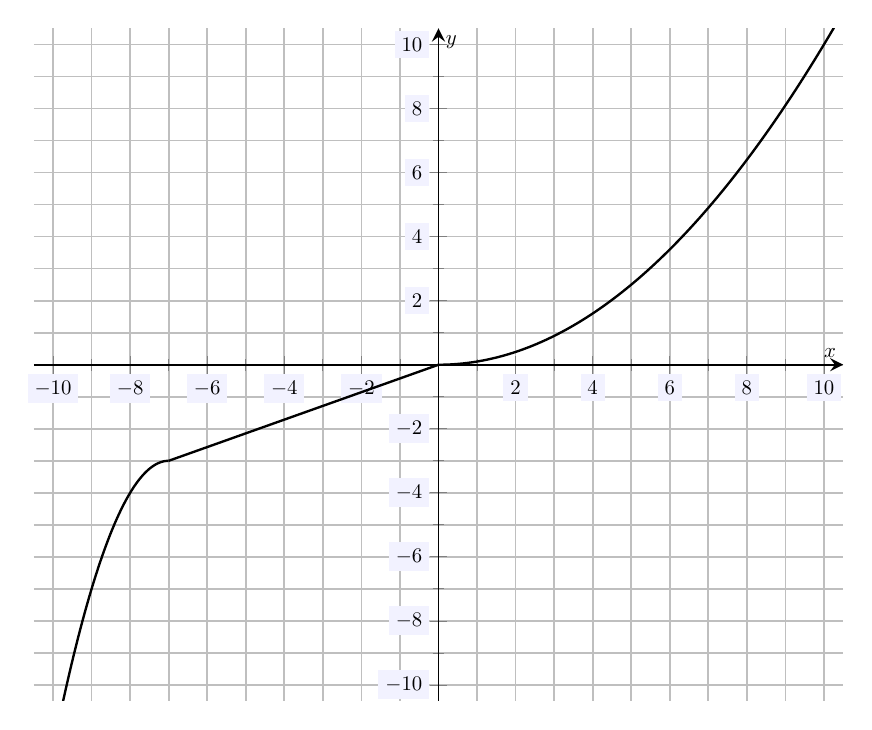
\begin{tikzpicture}[scale=1.5,every node/.style={scale=0.5}]
	\begin{axis}[
	grid=both,
	axis lines=middle,
	ticklabel style={fill=blue!5!white},
	xmin= -10.5, xmax=10.5,
	ymin= -10.5, ymax=10.5,
	xtick={-10,-8,-6,-4,-2,0,2,4,6,8,10},
	ytick={-10,-8,-6,-4,-2,0,2,4,6,8,10},
	minor tick = {-10,-9,...,10},
	xlabel=\(x\),ylabel=\(y\),
	]
	\addplot[line width= 0.02cm,samples=100,domain= -10.5:-7] ({x},{-(x + 7)^2 - 3}); 
	\addplot[line width= 0.02cm,samples=100,domain= -7:0] ({x},{3/7*x}); 
	\addplot[line width= 0.02cm,samples=100,domain= 0:10.5] ({x},{x^2/10}); 
	\end{axis}
	\end{tikzpicture}
	}
	\] 

\begin{enumerate}[(a)]
\item Compute $f(7)$ and $f(-9)$. 
\item Is $f(x)$ a function? Explain. 
\item Does $f(x)$ have an inverse? If so, sketch the inverse. If not, explain why. 
\end{enumerate} \pspace


% Problem 
\prob What does it mean for a function to be even? What does it mean for a function to be odd? What do these mean graphically? \pspace


% Problem
\prob Identify whether the following functions are even or odd algebraically:
	\begin{enumerate}[(a)]
	\item $f(x)= x^2 + 4$
	\item $g(x)= x^3 - x$
	\item $h(x)= 5$
	\item $j(x)= x^2 - x + 9$
	\end{enumerate} \pspace


% Problem
\prob Showing all the steps according to order of operations, compute the following:
	\begin{enumerate}[(a)]
	\item $10 + 10 - 16 \cdot 0 + 2 + 2$
	\item $(-1)^3 - 1 + 4^2/2$
	\item $15 - (6 - 10) + 3^2$
	\item $\dfrac{-4 - (2 - 4)^2}{3^2 - 1}$
	\end{enumerate} \pspace


% Problem
\prob Consider invertible functions $f, g$, whose values at several specified $x$-values are given below. 
	\begin{table}[h]
	\centering
	\begin{tabular}{|c||c|c|c|c|c|} \hline
	$x$ & $-6$ & $2$ & $0$ & $5$ & $9$ \\ \hline
	$f$ & $1$ & $5$ & $2$ & $-6$ & $3$ \\ \hline
	$g$ & $0$ & $2$ & $9$ & $1$ & $6$ \\ \hline
	\end{tabular}
	\end{table}
Find the following:
	\begin{enumerate}[(a)]
	\item $(f + g)(9)$
	\item $(f \circ g)(0)$
	\item $\left( \frac{g}{f} \right)(2)$
	\item $y$-intercept of $f(x)$
	\item An $x$-intercept of $g(x)$
	\end{enumerate} \pspace


% Problem
\prob Find the centers and radii for the following circles:
	\begin{enumerate}[(a)]
	\item $x^2 + (y - 4)^2= 36$
	\item $(x + 6)^2 + y^2= 4$
	\item $(x - 1)^2 + (y + 7)^2= 9$
	\item $(5 - x)^2 + (4 + y)^2= 10$
	\item $x^2 + (9 + y)^2= \dfrac{1}{\sqrt{2}}$
	\end{enumerate} \pspace


% Problem
\prob Define the following sets:
	\[
	\begin{aligned}
	A&= \{ 1,\; 2, \; 3,\; 4,\; 5,\; 6,\; 7,\; 8,\; 9,\; 10 \} \\
	B&= \{ 2,\; 4,\; 6,\; 8,\; 10 \} \\
	C&= \{ 1,\; 3,\; 5,\; 7,\; 9 \} \\
	D&= \{ 2,\; 3,\; 5,\; 7 \} \\
	E&= \{ 2,\; 3,\; 4,\; 6,\; 8,\; 9 \}
	\end{aligned}
	\]
Consider all these sets as subsets of $A$. Compute the following:
	\begin{enumerate}[(a)]
	\item $B \cup D$
	\item $C \cap E$
	\item $D \cup E$
	\item $A \cap B$
	\item $(B \cap C) \cup D$
	\item $D \cap (E \cap C)$
	\end{enumerate} \pspace


% Problem
\prob Define the following functions:
	\[
	\begin{aligned}
	f(x)&:= x^3 - x \\
	g(x)&:= x^2 - 2x + 3 \\
	h(x)&:= x^4 + x^2
	\end{aligned}
	\]
Determine if the functions $f(x)$, $g(x)$ and $h(x)$ are even functions, odd functions, or neither. Be sure to justify your answer. \pspace


% Problem
\prob Consider the function $f(x)$ plotted below. 
	\[
	\fbox{
	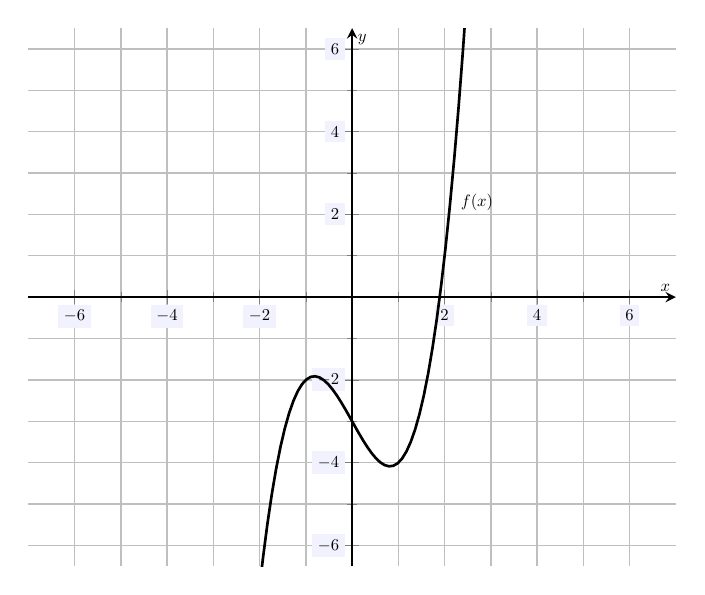
\begin{tikzpicture}[scale=1.2,every node/.style={scale=0.5}]
	\begin{axis}[
	grid=both,
	axis lines=middle,
	ticklabel style={fill=blue!5!white},
	xmin= -7, xmax=7,
	ymin= -6.5, ymax=6.5,
	xtick={-6,-4,-2,0,2,4,6},
	ytick={-6,-4,-2,0,2,4,6},
	minor tick = {-5,-3,...,5},
	xlabel=\(x\),ylabel=\(y\),
	samples=150
	]
	\node at (2.7,2.3) {$f(x)$};
	\addplot[thick,domain= -7:7] {x^3 - 2*x - 3};
	\end{axis}
	\end{tikzpicture}
	}
	\]

\begin{enumerate}[(a)]
\item What is $f(1)$? 
\item Is the point $(2,1)$ on the graph of $f(x)$? Explain. 
\item Is the point $(-2,-2)$ on the graph of $f(x)$? Explain. 
\item Is the function $f(x)$ even, odd, or neither. Explain. 
\end{enumerate} \pspace


% Problem
Define the following sets:
	\[
	\begin{aligned}
	A&= \text{All males over 40~years old.} & & & C&= \text{All US Presidents, alive or dead.} \\
	B&= \text{All people that have acted in a movie.} & & & D&= \text{All persons under 6~ft tall.} 
	\end{aligned}
	\]
Consider all of these sets as subsets of the set of all people alive. Being sure to completely justify your response, answer the following:
	\begin{enumerate}[(a)]
	\item Find an element of $A \cap B$. 
	\item Is Jeff Bezos~$\in A \cup C$? Is Jeff Bezos~$\in C \cup D$?
	\item Are sets $B$ and $C$ disjoint, i.e. is $B \cap C= \varnothing$? [Hint: Consider US~Presidents from the last 50~years.]
	\end{enumerate} \pspace


% Problem
\prob A lighthouse is located 7~mi due West and 3~mi due South of you. You will walk a straight path to the lighthouse at a rate of 2.5~mph. How long will it take you to walk to the lighthouse? \pspace


% Problem
\prob Showing all your work, simplify the following as much as possible---being sure that your answer involves no negative powers and all variables appear only once:
	\begin{enumerate}[(a)]
	\item $xy \sqrt{x^4 y^5}$
	\item $\dfrac{\sqrt{x^{10} y^5}}{\sqrt{x^2 y^3}}$
	\item $\sqrt[3]{x^{12} y^3 z^{11}}$
	\end{enumerate} \pspace


% Problem
\prob An oil company is selling off one of its oil reserves. The amount of oil left in the storage tank in tens of thousands of gallons, $O$, after $d$ days is given by $O(d)= 1600 - 133.4d$.
	\begin{enumerate}[(a)]
	\item Find and interpret the slope of $O(d)$ in the context of the problem.
	\item Find and interpret the $y$-intercept of $O(d)$ in the context of the problem.
	\item Find how long it will take the company to sell all the oil in the tank. 
	\item If the company sells the oil for \$2.085/gallon, how much money do they make selling this reserve oil?
	\end{enumerate} \pspace


% Problem
\prob Find the equation of the line with $x$-intercept $-6$ that passes through the point of intersection of $y= 5x - 1$ and $y= 6 - 2x$. \pspace


% Problem
\prob Solve the following equation:
	\[
	5\sqrt{2}\, x + 8= -3(1 - 2x)
	\] \pspace


% Problem
\prob Showing all your work, verify that $g(x)= 4x + 9$ is the inverse function for $f(x)= \frac{x - 9}{4}$. Also, compute $g(-2)$. What does the value of $g(-2)$ tell you about the function $f(x)$? \pspace


% Problem
\prob Determine whether the following relations are functions, being sure to justify your answer. If the relation is a function, determine its domain, codomain, and range. [For this problem, in determining a functions domain, codomain, and range, you may invoke the use/description of a graph.]
	\begin{enumerate}[(a)]
	\item \phantom{.}\par
	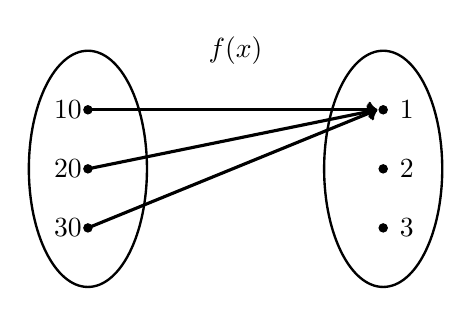
\begin{tikzpicture}[scale=0.75]
	\node at (2.5,2) {$f(x)$};
	% Ellipses
	\draw[line width=0.03cm] (0,0) circle (1 and 2);
	\draw[line width=0.03cm] (5,0) circle (1 and 2);
	
	% Nodes
	\draw[fill=black] (0,1) circle (0.07);
	\draw[fill=black] (0,0) circle (0.07);
	\draw[fill=black] (0,-1) circle (0.07);
	
	\draw[fill=black] (5,1) circle (0.07);
	\draw[fill=black] (5,0) circle (0.07);
	\draw[fill=black] (5,-1) circle (0.07);
	
	% Arrow
	\draw[line width=0.04cm,->] (0,1) -- (4.9,1);
	\draw[line width=0.04cm,->] (0,0) -- (4.9,1);
	\draw[line width=0.04cm,->] (0,-1) -- (4.9,1);
	
	% Labels
	\node at (-0.3,1) {$10\,$};
	\node at (-0.3,0) {$20\,$};
	\node at (-0.3,-1) {$30\,$};
	
	\node at (5.4,1) {$1$};
	\node at (5.4,0) {$2$};
	\node at (5.4,-1) {$3$};
	\end{tikzpicture}

	\item \phantom{.}\par
	\hspace{1cm}\begin{table}[H]
	\setlength\arrayrulewidth{0.02cm}
	\begin{tabular}{cc|r}
	\hspace{1cm} & $x$ & $g(x)$ \\ \cline{2-3} 
	& $1.0$ & $1.0$ \\
	& $1.5$ & $4.3$ \\
	& $3.0$ & $-6.1$ \\
	& $4.4$ & $2.2$ \\
	& $6.8$ & $1.0$ 
	\end{tabular}
	\end{table}
	
	\item $h(x, y)= x + y^4$. 
	
	\item $j(x)=$ the multiple of two closest to $x$.
	\end{enumerate} \pspace


% Problem
\prob Suppose that last year, the demand for a certain good was 185~thousand units. It is estimated that next year, the demand will be for 221~thousand units. 
	\begin{enumerate}[(a)]
	\item Assuming that the change in demand is constant, find a linear function predicting the level of demand $t$~years from now.
	\item Interpret the slope and $y$-intercept from your function in (a).
	\item What is your prediction for the level of demand in 5~years?
	\item Predict how many years until the demand is 400~thousand units. 
	\end{enumerate} \pspace


% Problem
\prob Let $f(x)$ be a function such that $f^{-1}(x)$ exists. A partial table of values for $f(x)$ is given below: \par
	\begin{table}[H]
	\centering
	\begin{tabular}{|r||c|c|c|c|c|} \hline 
	$x$ & $1$ & $2$ & $4$ & $8$ & $15$ \\ \hline
	$f(x)$ & $-2$ & $0$ & $6$ & $2$ & $10$ \\ \hline
	\end{tabular}
	\end{table}
Based on the table above (or your knowledge of functions and inverses), find the following:
	\begin{enumerate}[(a)]
	\item $f(2)$
	\item $f^{-1}(2)$
	\item $f^{-1}(f(2))$
	\item $f \big(f^{-1}(\pi) \big)$
	\item $f^{-1} \big( f(\sqrt{2}) \big)$
	\end{enumerate} \pspace


% Problem
\prob Let $f(x)= 5x - 4$. Find $f^{-1}(x)$. \pspace


% Problem
\prob Let $f(x)$ be the relation given by $f(x)= x(x - 1)(x + 3)$. 
	\begin{enumerate}[(a)]
	\item Is $f(x)$ a function? Explain. 
	\item Find $f(2)$.
	\item Find the $y$-intercept(s) of $f(x)$. 
	\item Find the $x$-intercept(s) of $f(x)$.
	\end{enumerate} \pspace


% Problem
\prob A graph of a relation $f(x)$ is shown below:
	\[
	\fbox{
	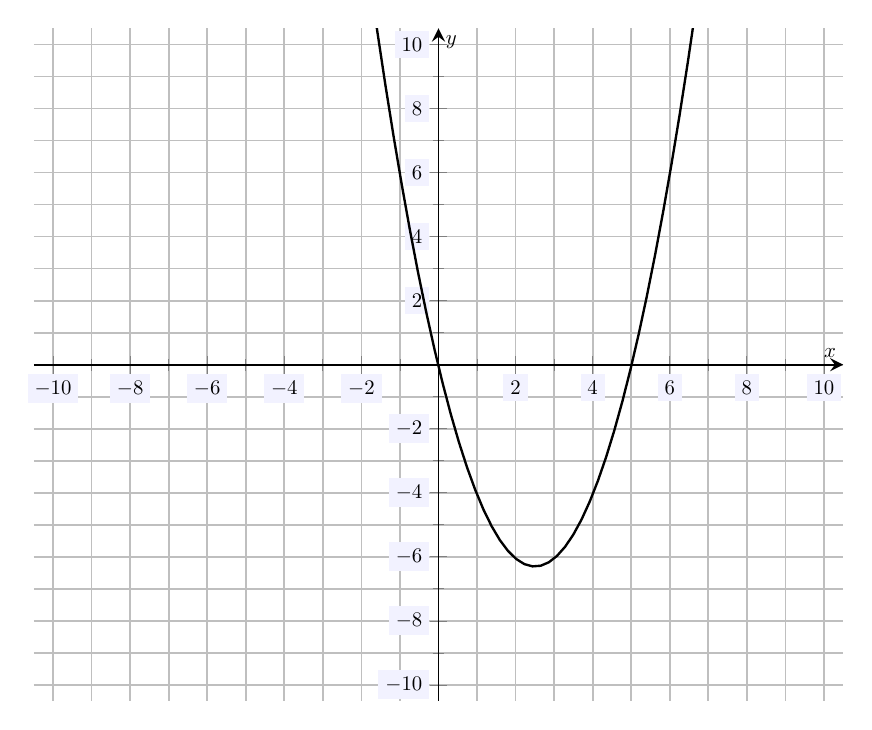
\begin{tikzpicture}[scale=1.5,every node/.style={scale=0.5}]
	\begin{axis}[
	grid=both,
	axis lines=middle,
	ticklabel style={fill=blue!5!white},
	xmin= -10.5, xmax=10.5,
	ymin= -10.5, ymax=10.5,
	xtick={-10,-8,-6,-4,-2,0,2,4,6,8,10},
	ytick={-10,-8,-6,-4,-2,0,2,4,6,8,10},
	minor tick = {-10,-9,...,10},
	xlabel=\(x\),ylabel=\(y\),
	]
	\addplot[line width= 0.02cm,samples=100,domain= -10.5:10.5] ({x},{(x - 2.5)^2 - 6.3}); 
	\end{axis}
	\end{tikzpicture}
	}
	\] 
Using the graph above, answer the following:
	\begin{enumerate}[(a)]
	\item Is the relation $f(x)$ a function? Explain.
	\item Does the relation $f(x)$ have an inverse function? Explain. 
	\end{enumerate} \pspace


% Problem
\prob Consider the function given by $f(x)= 11 - 9x$.
	\begin{enumerate}[(a)]
	\item Explain why $f^{-1}(x)$ exists. 
	\item Find $f^{-1}(x)$.
	\item Use $f^{-1}$ to solve the equation $f(x)= \frac{17}{9}$. 
	\end{enumerate} \pspace


% Problem
\prob Suppose $f(x)$ and $g(x)$ are the functions given below. 
	\[
	\begin{aligned}
	f(x)&= 2 - x \\[0.3cm]
	g(x)&= x^2 - 3x + 2
	\end{aligned}
	\]

Compute the following: \pspace
\begin{enumerate}[(a)]
\item $f(-4)=$ 
\item $g(2)=$ 
\item $2f(1) - g(3)=$ 
\item $f(x) - g(x)=$ 
\item $f(x) \, g(x)=$ 
\item $\left( \dfrac{f}{g} \right)(x)=$ 
\item $(f \circ g)(0)=$ 
\item $(g \circ f)(0)=$ 
\item $(f \circ g)(x)=$ 
\item $(g \circ f)(x)=$ 
\end{enumerate}  \pspace


% Problem
\prob Showing all your work, simplify the following as much as possible---being sure that your answer involves no negative powers and all variables appear only once:
	\begin{enumerate}[(a)]
	\item $(x^0 y^3)^2 \cdot (x^4 y^{-5})^{-2}$
	\item $\dfrac{x^{4} y^0 z^6}{(x z^2)^{-3}}$
	\item $\left( \dfrac{x^6 y^{-3} z}{(x z^2)^3 y^{-5}} \right)^{-2}$
	\end{enumerate} \pspace





\newpage





% Problem
\prob  Let $f(x)$ and $g(x)$ be functions for which a table of values is given below. \par
	\begin{table}[ht]
	\centering
	\begin{tabular}{|c||c|c|c|c|c|c|} \hline 
	$x$ & $-5$ & $-2$ & $0$ & $1$ & $2$ & $3$ \\ \hline \hline
	$f(x)$ & $\phantom{-}6$ & $-1$ & $\phantom{-}3$ & $4$ & $3$ & $-1$ \\ \hline
	$g(x)$ & $-5$ & $\phantom{-}7$ & $-2$ & $4$ & $0$ & $\phantom{-}6$ \\ \hline 
	\end{tabular}
	\end{table} \par
Based on the table above, compute the following:
	\begin{enumerate}[(a)]
	\item $f(-2) - g(3)$
	\item $(f + g)(2)$
	\item $(fg)(-5)$
	\item $(g \circ f)(0)$
	\item $(f \circ g)(0)$
	\end{enumerate} \pspace


% Problem
\prob Write down an expression that gives the equation for all linear functions passing through the point $(3, 5)$, then use this to find the line that passes through $(3, 5)$ and has $x$-intercept $-6$. \pspace


% Problem
\prob Let $g(x)= x^2 + 2x - 3$. 
	\begin{enumerate}[(a)]
	\item Find $g(2)$ and $g(-4)$.
	\item Based on your answer to (a), can $g^{-1}(x)$ exist? Explain. 
	\end{enumerate} \pspace


% Problem
\prob An \textit{arithmetic sequence} is a list of numbers where the difference between one number and the next is always the same. For instance, 2, 6, 10, 14, 18, \dots is an arithmetic sequence because the difference between sequential terms is always 4, while the sequence 1, 2, 3, 5, 7, 10, 13, \dots is \textit{not} an arithmetic sequence because the difference between sequential terms is not constant. Let $S$ be the sequence 34, 57, 80, 103, 126, \dots. 
	\begin{enumerate}[(a)]
	\item Find a function $S(n)$ that gives the $n$th term of the sequence. 
	\item Find the 835th term of the sequence. 
	\item Is 3,500 a term of this sequence? Explain. 
	\end{enumerate} \pspace


% Problem
\prob Showing all your work, simplify the following as much as possible: 
	\[
	\dfrac{\big( x^3 y^{-3} \big)^3 x^2 y^0}{x^{-3} \big( y^2 \big)^4}
	\] \pspace


% Problem
\prob You keep a secret lunchbox under your bed filled with cash. The lunchbox currently contains \$2,500. Each week, you place \$80 into the lunchbox. Let $M(w)$ denote the amount of money in the lunchbox $w$~weeks from now. 
	\begin{enumerate}[(a)]
	\item Explain why $M(w)$ is linear.
	\item Find $M(w)$. 
	\item Use (b) to find how long until the lunchbox has \$10,000. 
	\end{enumerate} \pspace


% Problem
\prob Showing all your work, simplify the following as much as possible: 
	\[
	x^4 y^3 \, \sqrt[4]{\dfrac{x^4 y^{-9}}{x^2 y^3}}
	\]  \pspace


% Problem
\prob You are driving home from university at 55~mph. Your home is 650~miles from your university. Assuming you left the university 2~hours ago and that you drive at a constant speed, find your distance from your home, $D(t)$, as function of time $t$, in hours. \pspace


% Problem
\prob A cleaning service does not have their prices listed on their website but the site does mention they charge a fixed amount per hour. You make some calls and have one friend that used their service and paid \$212.50 for a 3~hour cleaning while another friend paid \$400 for a 6~hour cleaning. Let $C(h)$ be the cost the service will charge for $h$~hours of cleaning.
	\begin{enumerate}[(a)]
	\item Explain why $C(h)$ is linear.
	\item Find $C(h)$.
	\item Interpret the slope and $y$-intercept for $C(h)$.
	\item How many hours of cleaning can you get for \$950?
	\end{enumerate} \pspace


% Problem
\prob Consider the function $\ell(x)= \dfrac{4 - 3x}{5}$. 
	\begin{enumerate}[(a)]
	\item Explain why $\ell(x)$ is linear. 
	\item Find the slope of this function.
	\item Find the $y$-intercept of this function.
	\item Find the $x$-intercept of this function.
	\item Does the graph of this function contain the point $(3, -1)$? Explain. 
	\end{enumerate} \pspace


% Problem 
\prob The amount of people, on average, that have entered a store $t$~hours after it has opened, $P(t)$, can be modeled by $P(t)= 30.5t - 4$. 
	\begin{enumerate}[(a)]
	\item What does $P(t)$ being linear imply about the rate that people enter the store?
	\item Find and interpret the slope and $y$-intercept of $I(s)$ in context, if possible.
	\item Find $P(2)$ and interpret the value. 
	\item How long after opening until 400~people have entered the store? 
	\end{enumerate} \pspace


% Problem
\prob A relation $\phi$ is plotted below. 
	\[
	\fbox{
	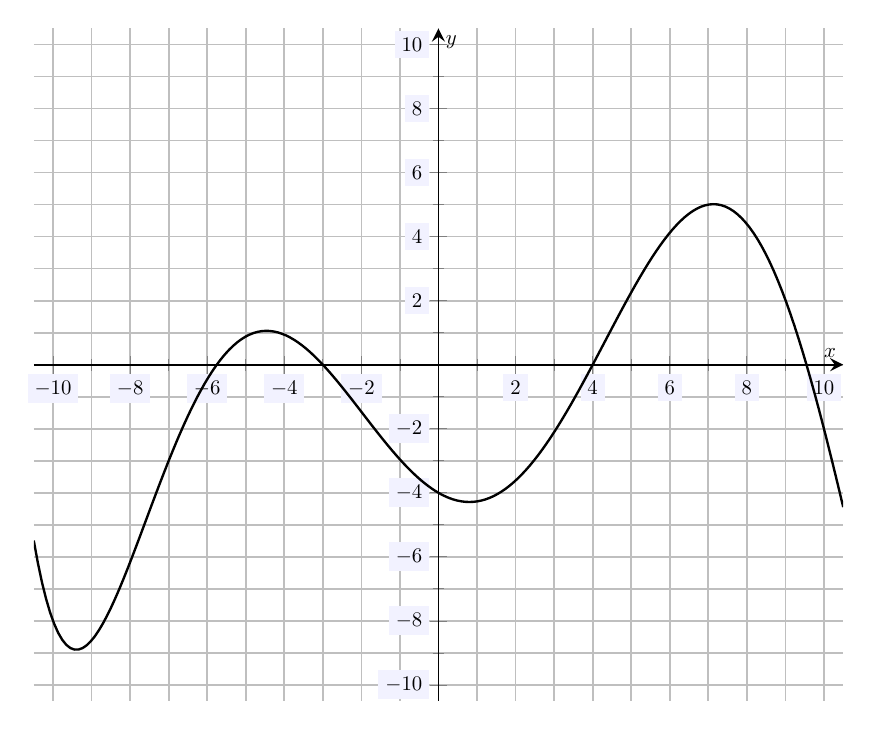
\begin{tikzpicture}[scale=1.5,every node/.style={scale=0.5}]
	\begin{axis}[
	grid=both,
	axis lines=middle,
	ticklabel style={fill=blue!5!white},
	xmin= -10.5, xmax=10.5,
	ymin= -10.5, ymax=10.5,
	xtick={-10,-8,-6,-4,-2,0,2,4,6,8,10},
	ytick={-10,-8,-6,-4,-2,0,2,4,6,8,10},
	minor tick = {-10,-9,...,10},
	xlabel=\(x\),ylabel=\(y\),
	]
	\addplot[line width= 0.02cm,samples=200,domain= -10.5:10.5] ({x},{-4. - 0.695759*x + 0.394934*x^2 + 0.0411407*x^3 - 0.00782987*x^4 - 0.000311831*x^5 + 0.0000378053*x^6}); 
	\end{axis}
	\end{tikzpicture}
	}
	\] 
Using the plot above, answer the following:
	\begin{enumerate}[(a)]
	\item Compute $\phi(9)$.
	\item Find the $y$-intercept for $\phi(x)$. 
	\item Find the $x$-intercepts for $\phi(x)$. 	
	\item As accurately as possible, compute the preimage of $-3$, i.e. $\phi^{-1}(-3)$. 
	\item Explain why (d) implies that $\phi$ does not have an inverse function. 
	\end{enumerate} \pspace


% Problem
\prob Let $f(x)$ be a function such that $f^{-1}(x)$ exists. A partial table of values for $f(x)$ is given below: \par
	\begin{table}[H]
	\centering
	\begin{tabular}{|r||c|c|c|c|c|} \hline 
	$x$ & $1$ & $2$ & $3$ & $4$ & $5$ \\ \hline
	$f(x)$ & $5$ & $7$ & $0$ & $9$ & $3$ \\ \hline
	\end{tabular}
	\end{table}
Based on the table above (or your knowledge of functions and inverses), find the following:
	\begin{enumerate}[(a)]
	\item $f(3)$
	\item $f^{-1}(3)$
	\item $f(4)$
	\item $f^{-1}(9)$
	\item $f(f^{-1}(5))$
	\item $f^{-1} \big( f(2) \big)$
	\item $f^{-1} \big( f(-8) \big)$
	\item $f \big( f^{-1}(10) \big)$
	\end{enumerate} \pspace


% Problem
\prob Suppose that $f(x, y)$ is the function given by the following table:
	\begin{table}[H]
	\centering
	\begin{tabular}{|c||r|r|r|r|} \hline 
	$x \backslash y$ & $1$ & $2$ & $3$ & $4$ \\ \hline \hline
	$1$ & $-2$ & $7$ & $4$ & $-4$ \\ \hline
	$2$ & $0$ & $3$ & $-1$ & $1$ \\ \hline
	$3$ & $5$ & $-6$ & $7$ & $6$ \\ \hline
	$4$ & $1$ & $0$ & $4$ & $0$ \\ \hline
	\end{tabular}
	\end{table} \par
Showing all your work, compute the following:
	\begin{enumerate}[(a)]
	\item $f(3, 2)$
	\item $f(3 - 1, 2^2)$
	\item $5 f(3, 1) - 8$
	\item $\dfrac{4 - f\big( 3^2 + (-2)^3, 1 \big) }{2 f(1, 3)}$
	\end{enumerate} \pspace


% Problem
\prob You and a coworker are responsible for maintaining a portion of a golf course. You can weed the field in 8~hours. When your coworker helps you, you are able to do it in 5~hours. How fast can your coworker weed the field? \pspace


% Problem
\prob Explain why the function $f(x)= 3(5 - 2x)$ has an inverse. Furthermore, find the inverse. Be sure to show all your work. [You do not need to verify that your inverse is indeed the inverse.] \pspace


% Problem
\prob You rent an apartment in NYC, which you paid a \$50 application fee to apply for. The rent is \$2500/month. Therefore, the amount you have paid, $R(t)$, to rent the apartment $t$ months after moving in is given by $R(t)= 2500t + 50$.
	\begin{enumerate}[(a)]
	\item Without knowing $R(t)$, how do you know that $R(t)$ is linear? 
	\item What is the slope of $R(t)$ and what does it represent in the problem context? 
	\item What is the $y$-intercept of $R(t)$ and what does it represent in the problem context? 
	\end{enumerate} \pspace


% Problem
\prob Let $\text{rdwn}(x)$ denote the largest integer that is {\itshape less than} $x$. 
	\begin{enumerate}[(a)]
	\item Find $\text{rdwn}(x)$ for $x= 0.5$, $2.2$, $5.9$, $6.0$, $-1.5$, $-4.9$, $-7$. 
	\item Explain why $\text{rdwn}(x)$ is a function.
	\item Being as accurate as possible, sketch a graph of $\text{rdwn}(x)$ on the plot below. 
	\[
	\fbox{%
	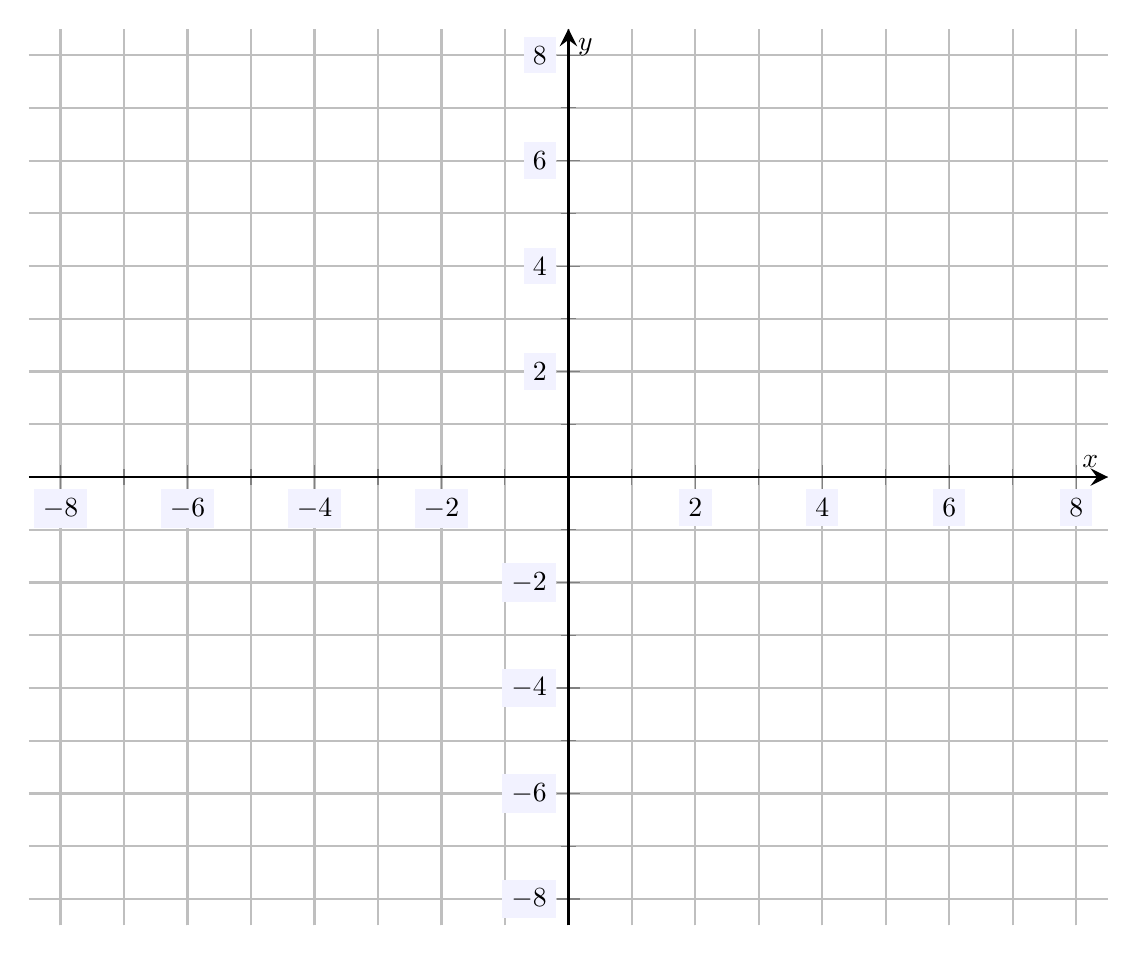
\begin{tikzpicture}[scale=2,every node/.style={scale=0.5}]
	\begin{axis}[
	grid=both,
	axis lines=middle,
	ticklabel style={fill=blue!5!white},
	xmin= -8.5, xmax=8.5,
	ymin= -8.5, ymax=8.5,
	xtick={-8,-6,-4,-2,0,2,4,6,8},
	ytick={-8,-6,-4,-2,0,2,4,6,8},
	minor tick = {-8,-7,...,8},
	xlabel=\(x\),ylabel=\(y\),
	]
	\end{axis}
	\end{tikzpicture}
	}
	\]
	\end{enumerate} \pspace


% Problem
\prob Define what it means to be a linear function. Then give an example of a linear function and evaluate it at some value. \pspace


% Problem
\prob Let $f(x)= x^2 + 2x - 1$, $g(x)= 3x + 8$, and $c$ be a constant. Showing all your work and simplifying as much as possible, compute the following:
	\begin{enumerate}[(a)]
	\item $(fg)(4)$
	\item $f(-2) - g(1)$
	\item $(f - g)(2)$
	\item $(f \circ g)(0)$
	\item $(g \circ f)(c)$
	\end{enumerate} \pspace


% Problem
\prob Find the exact equation of the line with $x$-intercept $-6$ and $y$-intercept $4$. Show all your work. \pspace


% Problem
\prob Consider the relation given by the diagram below.
	\[
	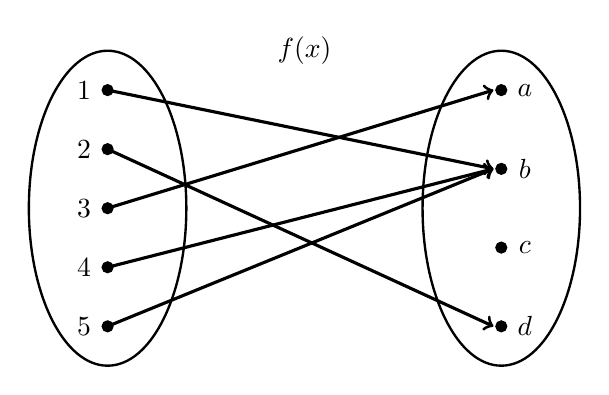
\begin{tikzpicture}
	\node at (2.5,2) {$f(x)$};
	
	% Ellipses
	\draw[line width=0.03cm] (0,0) circle (1 and 2);
	\draw[line width=0.03cm] (5,0) circle (1 and 2);
	
	% Nodes
	\draw[fill=black] (0,1.5) circle (0.07);
	\draw[fill=black] (0,0.75) circle (0.07);
	\draw[fill=black] (0,0) circle (0.07);
	\draw[fill=black] (0,-0.75) circle (0.07);
	\draw[fill=black] (0,-1.5) circle (0.07);
	
	\draw[fill=black] (5,1.5) circle (0.07);
	\draw[fill=black] (5,0.50) circle (0.07);
	\draw[fill=black] (5,-0.5) circle (0.07);
	\draw[fill=black] (5,-1.5) circle (0.07);
	
	% Arrow
	\draw[line width=0.04cm,->] (0,1.5) -- (4.9,0.50);
	\draw[line width=0.04cm,->] (0,0.75) -- (4.9,-1.5);
	\draw[line width=0.04cm,->] (0,0) -- (4.9,1.5);
	\draw[line width=0.04cm,->] (0,-1.5) -- (4.9,0.5);
	\draw[line width= 0.04cm,->,black] (0,-0.75) -- (4.9,0.5);
	
	% Labels
	\node at (-0.3,1.5) {$1$};
	\node at (-0.3,0.75) {$2$};
	\node at (-0.3,0) {$3$};
	\node at (-0.3,-0.75) {$4$};
	\node at (-0.3,-1.5) {$5$};
	
	\node at (5.3,1.5) {$a$};
	\node at (5.3,0.5) {$b$};
	\node at (5.3,-0.5) {$c$};
	\node at (5.3,-1.5) {$d$};
	\end{tikzpicture}
	\]

\begin{enumerate}[(a)]
\item Is the relation a function? Explain. 
\item Find the domain of the relation.
\item Find the codomain of the relation.
\item Find the range of the relation. 
\end{enumerate}  \pspace


% Problem
\prob Let $f(x)= \frac{1}{4} (x - 3)$. Assume that $f^{-1}(x)$ exists. 
	\begin{enumerate}[(a)]
	\item Find $f(15)$. 
	\item Use (a) to explain why $f^{-1}(3)= 15$. 
	\item Solve the equation given by $f(x)= 11$.
	\item Use (c) to explain why $f^{-1}(11)= 47$. 
	\end{enumerate} \pspace


% Problem
\prob Suppose $f(x)$ and $g(x)$ are the functions given below. 
        \begin{table}[H]
        \centering
        \begin{tabular}{| c || c | c | c | c | c | c | c |} \hline
	$x$ & $-3$ & $-2$ & $-1$ & $\phantom{-}0$ & $\phantom{-}1$ & $\phantom{-}2$ & $\phantom{-}3$ \\ \hline
	$f(x)$ & $\phantom{-1}4$ & $\phantom{-}2$ & $\phantom{-}0$ & $-5$ & $\phantom{-}1$ & $\phantom{-}2$ & $\phantom{-}4$ \\ \hline
	$g(x)$ & $\phantom{-1}2$ & $\phantom{-}1$ & $-1$ & $\phantom{-}1$ & $-2$ & $\phantom{-}3$ & $-3$ \\ \hline
	$h(x)$ & $-12$ & $\phantom{-}4$ & $\phantom{-}10$ & $-2$ & $\phantom{-}4$ & $-4$ & $\phantom{-}0$ \\ \hline
        \end{tabular}
        \end{table}

Compute the following: \pspace
        \begin{enumerate}[(a)]
        \item $(f + h)(-1)=$ 
        \item $(h - g)(2)=$ 
        \item $(5f)(2)=$ 
        \item $\left(\dfrac{h}{g}\right)(-3)=$ 
        \item $f(0)\, h(1)=$ 
        \item $g \big(2 - h(1) \big)=$ 
        \item $(f \circ g)(-3)=$ 
	\item $(g \circ h)(3)=$ 
        \item $(h \circ g)(3)=$ 
	\item $(f \circ g \circ h)(0)=$ 
        \end{enumerate}  \pspace


% Problem
\prob Suppose $f(x)$ is the function given below.
	\[
	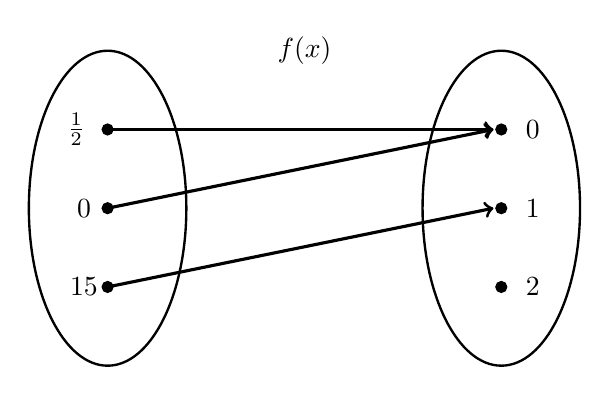
\begin{tikzpicture}
	\node at (2.5,2) {$f(x)$};
	% Ellipses
	\draw[line width=0.03cm] (0,0) circle (1 and 2);
	\draw[line width=0.03cm] (5,0) circle (1 and 2);
	
	% Nodes
	\draw[fill=black] (0,1) circle (0.07);
	\draw[fill=black] (0,0) circle (0.07);
	\draw[fill=black] (0,-1) circle (0.07);
	
	\draw[fill=black] (5,1) circle (0.07);
	\draw[fill=black] (5,0) circle (0.07);
	\draw[fill=black] (5,-1) circle (0.07);
	
	% Arrow
	\draw[line width=0.04cm,->] (0,1) -- (4.9,1);
	\draw[line width=0.04cm,->] (0,0) -- (4.9,1);
	\draw[line width=0.04cm,->] (0,-1) -- (4.9,0);
	
	% Labels
	\node at (-0.4,1) {$\frac{1}{2}$};
	\node at (-0.3,0) {$0$};
	\node at (-0.3,-1) {$15$};
	
	\node at (5.4,1) {$0$};
	\node at (5.4,0) {$1$};
	\node at (5.4,-1) {$2$};
	\end{tikzpicture}
	\]

\begin{enumerate}[(a)]
\item Explain why $f(x)$ is a function.
\item Find the value of $f(x)$ on each value in its domain. 
\item What is the domain of $f(x)$?
\item What is the codomain of $f(x)$?
\item What is the range of $f(x)$?
\end{enumerate} \pspace


% Problem
\prob Find the equation of the line with $x$-intercept $-7$ and $y$-intercept 3. \pspace 


% Problem
\prob Let $y= \frac{1}{3}\,x + 5$.
	\begin{enumerate}[(a)]
	\item By interchanging the roles of $y$ and $x$, find the inverse to the function $f(x)= \frac{1}{3}\,x + 5$.
	\item Use the answer from (a) to find $f^{-1}(-2)$. 
	\end{enumerate} \pspace


% Problem
\prob Richard is a tailor. He uses an automated sewing machine can create custom labels on jackets. Every 4~hours, it is able to stitch 26~jackets. Richard sets the machine going during the night and when he comes in the next morning it has stitched 80~jackets.
	\begin{enumerate}[(a)]
	\item Assuming the machine works at a constant rate, find the number of jackets, $J$, that the machine has stitched $t$~hours from now.
	\item How many total jackets has the machine stitched 8~hours after opening?
	\end{enumerate} \pspace


% Problem
\prob Consider the relation plotted below.
	\[
	\fbox{
	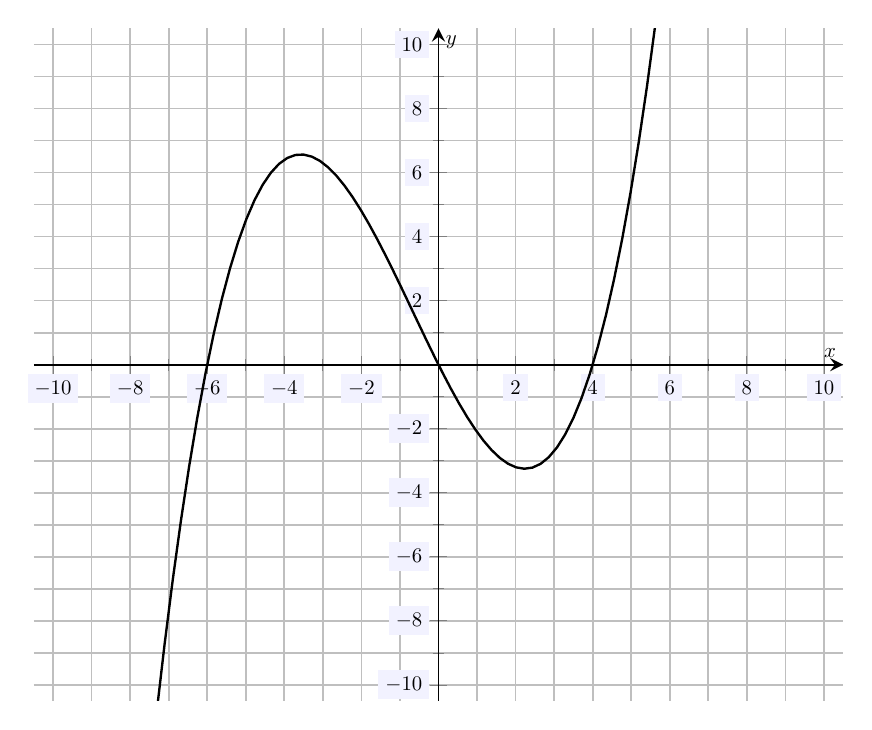
\begin{tikzpicture}[scale=1.5,every node/.style={scale=0.5}]
	\begin{axis}[
	grid=both,
	axis lines=middle,
	ticklabel style={fill=blue!5!white},
	xmin= -10.5, xmax=10.5,
	ymin= -10.5, ymax=10.5,
	xtick={-10,-8,-6,-4,-2,0,2,4,6,8,10},
	ytick={-10,-8,-6,-4,-2,0,2,4,6,8,10},
	minor tick = {-10,-9,...,10},
	xlabel=\(x\),ylabel=\(y\),
	]
	\addplot[line width= 0.02cm,samples=100,domain= -10.5:10.5] ({x},{1/10*x*(x + 6)*(x-4)});
	\end{axis}
	\end{tikzpicture}
	}
	\] 

\begin{enumerate}[(a)]
\item Is this relation a function of $x$? Explain.
\item Is this relation a function of $y$? Explain. 
\item If one were to consider this relation as a function of $x$, would the relation have an inverse? Explain. 
\end{enumerate} \pspace


% Problem
\prob Find the exact equation of the line parallel to the line $4x - 3y= 6$ whose graph contains the point $(-9, -8)$. Show all your work. \pspace


% Problem 
\prob Consider the function $f(x)= 121.5 - 11.6x$. 
	\begin{enumerate}[(a)]
	\item Explain why $f(x)$ is linear.
	\item Find the slope and $y$-intercept of $f(x)$.
	\item Find $f(x)$ when $x= 7.2$
	\end{enumerate} \pspace


% Problem
\prob Find the equation of the linear function which passes through the points $(-4, 10)$ and $(6, -8)$. \pspace


% Problem
\prob Suppose $f(x)$ and $g(x)$ are functions. 
	\begin{enumerate}[(a)]
	\item Explain what it means for $f(2)= g(2)$ graphically. 
	\item Explain what $f(x)$ and $g(x)$ intersecting at the point $(-1, 7)$ means algebraically. 
	\end{enumerate} \pspace


% Problem
\prob Explain why $f(x, y)= 2x^2 - y^3 + 6$ is a function. Then find $f(0, 0)$, $f(3, -1)$, $f(-3, 2)$, and $f(1, 1)$. \pspace


% Problem
\prob Solve the following equation and check your solution:
	\[
	\dfrac{x - 3}{1 - x}= 5
	\] \pspace


% Problem
\prob Find the equation of the line perpendicular to $y= \dfrac{5 - 3x}{6}$ whose graph passes through the $x$-intercept of the line $-3x + 9y= 15$. Show all your work. \pspace


% Problem
\prob Let $f(x)= 5 - 6x$. Assume that $f^{-1}(x)$ exists and observe that $f(2)= -7$.
	\begin{enumerate}[(a)]
	\item What is $f^{-1}(-7)$? Explain. 
	\item Find $f^{-1}(17)$.
	\end{enumerate} \pspace


% Problem
\prob Jeffrey is writing a term paper. Currently, he has only written 8~pages. He returns from a writing break and then goes back to the paper. After an additional 5~hours of writing, he has written 20~pages. 
	\begin{enumerate}[(a)]
	\item Assuming Jeffrey writes at a constant rate, find the linear function representing the number of pages that he has written after $t$ hours of writing. 
	\item How long after this break will it take him in total to write this 50~page term paper?
	\end{enumerate}  \pspace


% Problem 
\prob Find the equation of the linear function with slope $-15$ and $y$-intercept 19. \pspace


% Problem
\prob A function $f(x)$ has a table of values given below. Using this table, explain why $f^{-1}(x)$ cannot exist. \par
	\begin{table}[H]
	\centering
	\begin{tabular}{|r||c|c|c|c|c|} \hline
	$x$ & $1$ & $2$ & $3$ & $4$ & $5$ \\ \hline
	$f(x)$ & $6$ & $3$ & $9$ & $6$ & $1$ \\ \hline
	\end{tabular}
	\end{table} \pspace


% Problem
\prob A graph of a relation $f(x)$ is shown below:
	\[
	\fbox{
	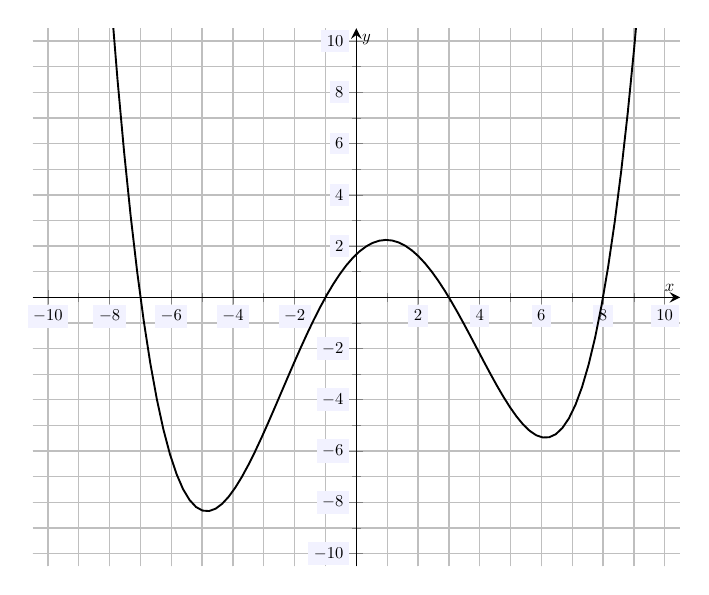
\begin{tikzpicture}[scale=1.2,every node/.style={scale=0.5}]
	\begin{axis}[
	grid=both,
	axis lines=middle,
	ticklabel style={fill=blue!5!white},
	xmin= -10.5, xmax=10.5,
	ymin= -10.5, ymax=10.5,
	xtick={-10,-8,-6,-4,-2,0,2,4,6,8,10},
	ytick={-10,-8,-6,-4,-2,0,2,4,6,8,10},
	minor tick = {-10,-9,...,10},
	xlabel=\(x\),ylabel=\(y\),
	]
	\addplot[line width= 0.02cm,samples=100,domain= -10.5:10.5] ({x},{1/100*(x+7)*(x+1)*(x-3)*(x-8)}); 
	\end{axis}
	\end{tikzpicture}
	}
	\] 
Using the graph above, answer the following:
	\begin{enumerate}[(a)]
	\item Is the relation $f(x)$ a function? Explain.
	\item Does the relation $f(x)$ have an inverse function? Explain. 
	\end{enumerate} \pspace


% Problem
\prob Solve the following equation:
	\[
	3(x - 1)= 1 - 8x
	\] \pspace


% Problem
\prob Find the equation of the line with slope $-\frac{2}{3}$ that passes through the point $(-9 ,10)$. \pspace


% Problem
\prob Let $f(x)= 4x + 3$ and $g(x)= \frac{1}{4}(x - 3)$. Show that $g(x)$ is the inverse of $f(x)$ by showing that $(f \circ g)(x)= f(g(x))= x$ and $(g \circ f)(x)= x$.  \pspace


% Problem
\prob Suppose that the number of people, $N$ that have ridden the subway $t$~hours after 8:00~am can be modeled by $N(t)= 8429t - 1008$. 
	\begin{enumerate}[(a)]
	\item Find and interpret the slope of $N(t)$.
	\item Does the $y$-intercept of $N(t)$ have an interpretation in the context of this problem? Explain.
	\item Find the number of people that have ridden the subway by 5~pm. 
	\end{enumerate} \pspace


% Problem
\prob Find the equation of the line passing through the points $(-5, 8)$ and $(7, 8)$. \pspace


% Problem
\prob Determine whether the relations $F$ and $G$ shown below are functions. Be sure to fully justify your answer. \pspace
	\hfill
	\begin{minipage}[c]{0.48\textwidth}
	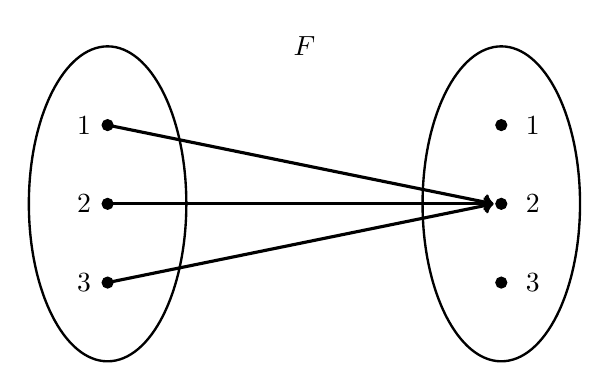
\begin{tikzpicture}
	\node at (2.5,2) {$F$};
	% Ellipses
	\draw[line width=0.03cm] (0,0) circle (1 and 2);
	\draw[line width=0.03cm] (5,0) circle (1 and 2);
	
	% Nodes
	\draw[fill=black] (0,1) circle (0.07);
	\draw[fill=black] (0,0) circle (0.07);
	\draw[fill=black] (0,-1) circle (0.07);
	
	\draw[fill=black] (5,1) circle (0.07);
	\draw[fill=black] (5,0) circle (0.07);
	\draw[fill=black] (5,-1) circle (0.07);
	
	% Arrow
	\draw[line width=0.04cm,->] (0,1) -- (4.9,0);
	\draw[line width=0.04cm,->] (0,0) -- (4.9,0);
	\draw[line width=0.04cm,->] (0,-1) -- (4.9,0);
	
	% Labels
	\node at (-0.3,1) {$1$};
	\node at (-0.3,0) {$2$};
	\node at (-0.3,-1) {$3$};
	
	\node at (5.4,1) {$1$};
	\node at (5.4,0) {$2$};
	\node at (5.4,-1) {$3$};
	\end{tikzpicture}
	\end{minipage}%
	\begin{minipage}[c]{0.40\textwidth}
	\begin{table}[H]
	\centering
	\begin{tabular}{cc}
	$x$ & $G$ \\ \hline
	$1$ & $0$ \\
	$2$ & $2$ \\
	$3$ & $4$ \\
	$4$ & $7$ \\
	$5$ & $0$
	\end{tabular}
	\end{table}
	\end{minipage} \pspace


% Problem
\prob Give an example of a `real world' relationship between two variables which does represent a functional relationship. Also, give an example of a `real world' relationship between two variables which \textit{does not} represent a functional relationship. Be sure to fully explain your responses. \pspace


% Problem
\prob  Let $f(x)= \dfrac{7 - x}{2}$ and $g(x)= 7 - 2x$. Show that $g(x)$ is the inverse of $f(x)$. \pspace


% Problem
\prob Solve the following equation and verify your solution:
	\[
	4(x - 2)= 5 - 9x
	\] \pspace


% Problem
\prob Let $\ell(x)= 18.2 - 13.7x$. Find the slope and $y$-intercept of this function.  \pspace


% Problem
\prob Let $\ell(x)= 57.6x - 1654.8$. Explain why $\ell(x)$ is a linear function. Find the $y$-intercept and $x$-intercept of this function. \pspace


% Problem
\prob Showing all your work, simplify the following as much as possible---being sure that your answer involves no negative powers and all variables appear only once:
	\begin{enumerate}[(a)]
	\item $\sqrt[3]{x^3 y^2} \cdot \sqrt{x y^3}$
	\item $\left( \dfrac{x^5}{\sqrt{x}} \right)^{2/3}$
	\item $xy \left( \sqrt{\dfrac{x^2}{y^3}} \right)^{-4}$
	\end{enumerate} \pspace


% Problem
\prob Suppose you work an hourly job where you are paid \$17.50 an hour. You have already made \$288.75 this week. Let $W$ represent the wages you have been paid by working an addition $h$ hours this week.
	\begin{enumerate}[(a)]
	\item Explain why $W$ is a linear function of $h$. 
	\item Explain why $W(h)= 17.50h + 288.75$.
	\item What is the slope and what does it represent?
	\item What is the $y$-intercept and what does it represent?
	\end{enumerate} \pspace


% Problem
\prob Let $M$ represent the total amount of money in your account $d$ days from now. Suppose that right now you have \$15,000 in your account and that you spend \$530 a day.
	\begin{enumerate}[(a)]
	\item Find $M(d)$.
	\item What are the slope and $y$-intercept of $M(d)$? What do they represent?
	\item Find the $x$-intercept of $M(d)$.
	\item Interpret your answer in (c). 
	\end{enumerate} \pspace


% Problem
\prob Louise just read \textit{Remembrance of Things Past} by Marcel Proust, which is approximately 3,200~pages long. She kept careful track of the time she was at various pages. She found that she count model the amount of pages she had read, $P$, after $t$ hours by $P(t)= 65t$.
	\begin{enumerate}[(a)]
	\item Find and interpret the slope of $P(t)$.
	\item Find and interpret the $y$-intercept of $P(t)$.
	\item How long did it take her to read this work?
	\end{enumerate} \pspace


% Problem
\prob Do you think a person's height is a function of time? Do you think a person's salary is a function of their body temperature? For each, explain why or why not. \pspace


% Problem
\prob Determine if the relations $f(x)$ and $g(x)$ shown below are functions. Explain why or why not. 
	\[
	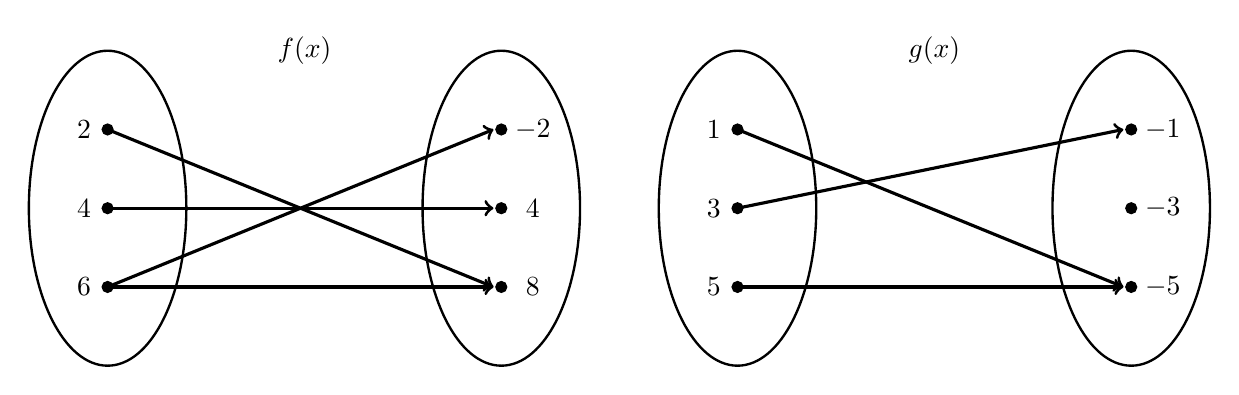
\begin{tikzpicture}
	\node at (2.5,2) {$f(x)$};
	% Ellipses
	\draw[line width=0.03cm] (0,0) circle (1 and 2);
	\draw[line width=0.03cm] (5,0) circle (1 and 2);
	
	% Nodes
	\draw[fill=black] (0,1) circle (0.07);
	\draw[fill=black] (0,0) circle (0.07);
	\draw[fill=black] (0,-1) circle (0.07);
	
	\draw[fill=black] (5,1) circle (0.07);
	\draw[fill=black] (5,0) circle (0.07);
	\draw[fill=black] (5,-1) circle (0.07);
	
	% Arrow
	\draw[line width=0.04cm,->] (0,1) -- (4.9,-1);
	\draw[line width=0.04cm,->] (0,0) -- (4.9,0);
	\draw[line width=0.04cm,->] (0,-1) -- (4.9,1);
	\draw[line width=0.04cm,->] (0,-1) -- (4.9,-1);
	
	% Labels
	\node at (-0.3,1) {$2$};
	\node at (-0.3,0) {$4$};
	\node at (-0.3,-1) {$6$};
	
	\node at (5.4,1) {$-2$};
	\node at (5.4,0) {$4$};
	\node at (5.4,-1) {$8$};
	
	\tikzset{shift={(8,0)}}
	%
	\node at (2.5,2) {$g(x)$};
	% Ellipses
	\draw[line width=0.03cm] (0,0) circle (1 and 2);
	\draw[line width=0.03cm] (5,0) circle (1 and 2);
	
	% Nodes
	\draw[fill=black] (0,1) circle (0.07);
	\draw[fill=black] (0,0) circle (0.07);
	\draw[fill=black] (0,-1) circle (0.07);
	
	\draw[fill=black] (5,1) circle (0.07);
	\draw[fill=black] (5,0) circle (0.07);
	\draw[fill=black] (5,-1) circle (0.07);
	
	% Arrow
	\draw[line width=0.04cm,->] (0,1) -- (4.9,-1);
	\draw[line width=0.04cm,->] (0,0) -- (4.9,1);
	\draw[line width=0.04cm,->] (0,-1) -- (4.9,-1);
	
	% Labels
	\node at (-0.3,1) {$1$};
	\node at (-0.3,0) {$3$};
	\node at (-0.3,-1) {$5$};
	
	\node at (5.4,1) {$-1$};
	\node at (5.4,0) {$-3$};
	\node at (5.4,-1) {$-5$};
	\end{tikzpicture}
	\] \pspace


% Problem
\prob Consider the line $2x - 5y= 4$.
	\begin{enumerate}[(a)]
	\item Is $(-2, 0)$ on the line? Explain.
	\item Is $(-3, -2)$ on the line? Explain.
	\item Showing all your work, find two points, distinct from $(-2, 0)$ and $(-3, -2)$, on the given line. 
	\end{enumerate} \pspace


% Problem
\prob Define the following sets:
	\[
	\begin{aligned}
	A&= \{ -3,\; 1, \; 2,\; 3,\; 5,\; 10,\; 20,\; 30,\; 40,\; 50 \} \\
	B&= \{ -3,\; 3,\; 10,\; 50 \} \\
	C&= \{ 2,\; 5,\; 20,\; 40,\; 50 \} \\
	D&= \{ -3,\; 1,\; 5 \} \\
	E&= \{ 1,\; 2,\; 3,\; 5 \}
	\end{aligned}
	\]
Consider all these sets as subsets of $A$. Compute the following:
	\begin{enumerate}[(a)]
	\item $A \cap B$
	\item $C \cup D$
	\item $D \cap E$
	\item $B \cap (D \cup E)$
	\end{enumerate} \pspace


% Problem
\prob Determine if the relations $f(x)$ and $g(x)$ shown below are functions. Explain why or why not. If the relation is a function, compute the functions value at $x= -4.1$.  \pspace


% Problem
\prob Find the linear function through the points $(-1, 6)$ and $(3, -4)$. Is this linear function increasing or decreasing? Explain. \pspace


% Problem
\prob For each of the following, describe whether the given dependent variable is a function of the independent variable:
	\begin{enumerate}[(a)]
	\item Independent: Number of stains removed by a test detergent. 
		Dependent: Type of detergent used. 
	\item Independent: Time since the song began.
		Dependent: Number of words spoken in the song. 
	\item Independent: Phase of the moon.
		Dependent: Day of the week. 
	\item Independent: Number of days since an account was opened. 
		Dependent: Amount of money in the account. 
	\end{enumerate} \pspace


% Problem
\prob Determine whether the relation below is a function of not. Be sure to fully justify your response. If the relation is a function, find its domain, codomain, and range. 
	\[
	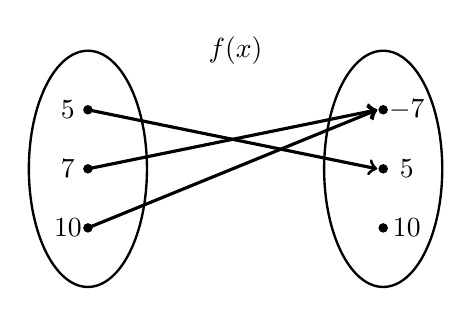
\begin{tikzpicture}[scale=0.75]
	\node at (2.5,2) {$f(x)$};
	% Ellipses
	\draw[line width=0.03cm] (0,0) circle (1 and 2);
	\draw[line width=0.03cm] (5,0) circle (1 and 2);
	
	% Nodes
	\draw[fill=black] (0,1) circle (0.07);
	\draw[fill=black] (0,0) circle (0.07);
	\draw[fill=black] (0,-1) circle (0.07);
	
	\draw[fill=black] (5,1) circle (0.07);
	\draw[fill=black] (5,0) circle (0.07);
	\draw[fill=black] (5,-1) circle (0.07);
	
	% Arrow
	\draw[line width=0.04cm,->] (0,1) -- (4.9,0);
	\draw[line width=0.04cm,->] (0,0) -- (4.9,1);
	\draw[line width=0.04cm,->] (0,-1) -- (4.9,1);
	
	% Labels
	\node at (-0.3,1) {$5\,$};
	\node at (-0.3,0) {$7\,$};
	\node at (-0.3,-1) {$10\,$};
	
	\node at (5.4,1) {$-7$};
	\node at (5.4,0) {$5$};
	\node at (5.4,-1) {$10$};
	\end{tikzpicture}
	\] \pspace


% Problem
\prob Explain why $f(x, y)= x^2 - y + 1$ is a function. Then showing all your work, find $f(0, 0)$, $f(0, -4)$, $f(3, 6)$, and $f(-2, 10)$. \pspace


% Problem
\prob Consider the line $-3x - 5y= 10$.
	\begin{enumerate}[(a)]
	\item Find the slope of the line.
	\item Find the $y$-intercept of the line.
	\item Find this line as a linear function, $f(x)$.
	\item Using your $f(x)$ from (c), find a point on the line distinct from the $y$-intercept.
	\end{enumerate} \pspace


% Problem
\prob Determine whether the point $(-6, -2)$ is on the graph of $f(x)= 8 - \frac{5}{3}\,x$. Determine also whether the point $(12, -12)$ is on the graph of $f(x)$. For each, explain why or why not. \pspace


% Problem
\prob An oil company is selling off oil in one of their reserves. The amount of oil in the tank in gallons, $O$, after $d$ days is given by $O(d)= 180000 - 19000d$.
	\begin{enumerate}[(a)]
	\item Find and interpret the slope of $O(d)$ in the context of the problem. 
	\item Find and interpret the $y$-intercept of $O(d)$ in the context of the problem. 
	\end{enumerate} \pspace


% Problem
\prob Showing all your work, simplify the expressions given below. Your answer should have each variable occurring at most once and should contain no negative powers.
	\begin{enumerate}[(a)]
	\item $\dfrac{(x y^5)^{-2}}{x^{-8} (x y)^6 y^5}$
	\item $\left( \dfrac{x (x^{10} y^{3})^0}{y^5} \right)^{-2}$
	\item $\dfrac{x \left( x^3 (y^{-2} z)^{-2} \right)^{-1}}{y^{-5} z^{2} x^{-1}}$
	\end{enumerate} \pspace


% Problem
\prob Showing all your work, simplify the expressions given below. Your answer should have each variable occurring at most once, contain no negative powers, and contain no fractional powers:
	\begin{enumerate}[(a)]
	\item $\dfrac{\sqrt{x^4 y^{11}}}{x \sqrt{y}}$
	\item $\left( \dfrac{x^5 y^8}{x^{-2} y^5} \right)^{-1/3}$
	\item $\dfrac{\sqrt[5]{x^{20} y^6}}{x^{10} \sqrt{y^3}}$
	\end{enumerate} \pspace


% Problem
\prob Suppose $f(x)$ is the relation given below.
	\[
	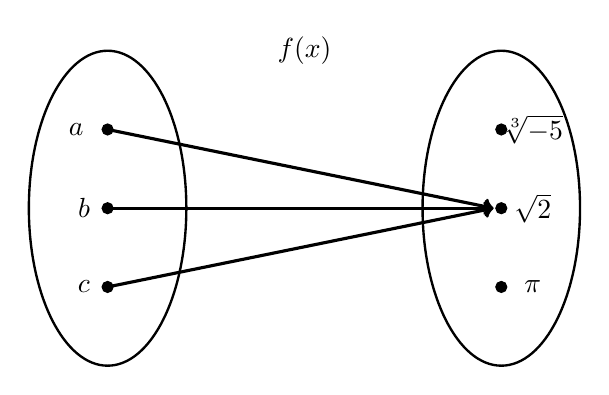
\begin{tikzpicture}
	\node at (2.5,2) {$f(x)$};
	% Ellipses
	\draw[line width=0.03cm] (0,0) circle (1 and 2);
	\draw[line width=0.03cm] (5,0) circle (1 and 2);
	
	% Nodes
	\draw[fill=black] (0,1) circle (0.07);
	\draw[fill=black] (0,0) circle (0.07);
	\draw[fill=black] (0,-1) circle (0.07);
	
	\draw[fill=black] (5,1) circle (0.07);
	\draw[fill=black] (5,0) circle (0.07);
	\draw[fill=black] (5,-1) circle (0.07);
	
	% Arrow
	\draw[line width=0.04cm,->] (0,1) -- (4.9,0);
	\draw[line width=0.04cm,->] (0,0) -- (4.9,0);
	\draw[line width=0.04cm,->] (0,-1) -- (4.9,0);
	
	% Labels
	\node at (-0.4,1) {$a$};
	\node at (-0.3,0) {$b$};
	\node at (-0.3,-1) {$c$};
	
	\node at (5.4,1) {$\sqrt[3]{-5}$};
	\node at (5.4,0) {$\sqrt{2}$};
	\node at (5.4,-1) {$\pi$};
	\end{tikzpicture}
	\]

\begin{enumerate}[(a)]
\item Is $f(x)$ a function? Explain.
\item What is the domain of $f(x)$?
\item What is the codomain of $f(x)$?
\item What is the range of $f(x)$?
\end{enumerate} \pspace


% Problem
\prob Is $f(x)= \dfrac{1 - x^3}{x^2 + 5}$ a function? Explain. \pspace


% Problem
\prob Consider the linear function $f(x)= 7 - \frac{6}{7}\, x$.
	\begin{enumerate}[(a)]
	\item Find the rate of change of $f(x)$.
	\item Is $f(x)$ increasing or decreasing? Explain.
	\item Find the $y$-intercept of $f(x)$.
	\item Find $f(-3)$.
	\end{enumerate} \pspace


% Problem
\prob Showing all your work, simplify the following as much as possible---being sure that your answer involves no negative powers and all variables appear only once:
	\begin{enumerate}[(a)]
	\item $(y \sqrt{x})^4 \cdot (x^{-3} y^2)^{-1}$
	\item $(x \sqrt{y}) \cdot (y \sqrt[3]{x})$
	\item $\left( \dfrac{x \sqrt{y^5}}{y^2 \sqrt{x^6}} \right)^{-1/2}$
	\end{enumerate} \pspace


% Problem
\prob Consider the function $f(x)= 9 - 2x$. 
	\begin{enumerate}[(a)]
	\item Explain why $f(x)$ is a linear function. 
	\item Find the slope and $y$-intercept for $f(x)$. 
	\item Find the $x$-intercept for $f(x)$. 
	\item Find $f(3)$. 
	\item Find an $x$ such that $f(x)= 5$. 
	\end{enumerate} \pspace


% Problem
\prob Let $f(x, y)= (x - y)^2 - x + \dfrac{10}{y}$. Find $f(3, -2)$ and $f(4, 5)$. \pspace


% Problem
\prob Let $f(x)= 4 - x^3$ and observe that $f(2)= -4$. 
	\begin{enumerate}[(a)]
	\item Is $(-1, 3)$ on the graph of $f(x)$? Explain. 
	\item Is $(2, -4)$ on the graph of $f(x)$? Explain. 
	\end{enumerate} \pspace


% Problem
\prob Suppose $f(x)$ and $g(x)$ are the functions given below. 
        \begin{table}[H]
        \centering
        \begin{tabular}{| c || c | c | c | c | c | c | c |} \hline
	$x$ & $-3$ & $-2$ & $-1$ & $\phantom{-}0$ & $\phantom{-}1$ & $\phantom{-}2$ & $\phantom{-}3$ \\ \hline
	$f(x)$ & $\phantom{-}0$ & $\phantom{-}5$ & $\phantom{-}4$ & $-1$ & $-5$ & $-1$ & $-3$ \\ \hline
	$g(x)$ & $\phantom{-}1$ & $\phantom{-}2$ & $10$ & $\phantom{-}3$ & $\phantom{-}4$ & $-7$ & $\phantom{-}5$  \\ \hline
        \end{tabular}
        \end{table}

Compute the following: 
        \begin{enumerate}[(a)]
	\item $(f - g)(-1)$
	\item $(fg)(2)$
	\item $(-5g)(-2)$
	\item $(f \circ g)(0)$
	\item $(g \circ f)(0)$
        \end{enumerate} \pspace


% Problem
\prob Using the plot of the linear function $f(x)$ below, answer the following: 
        \begin{enumerate}[(a)]
        \item Find the slope of the given line.
        \item Find the $y$-intercept of the given line.
        \item Find $f(x)$.
        \item Find the $x$-intercept of $f(x)$. 
        \end{enumerate}
	\[
	\fbox{
	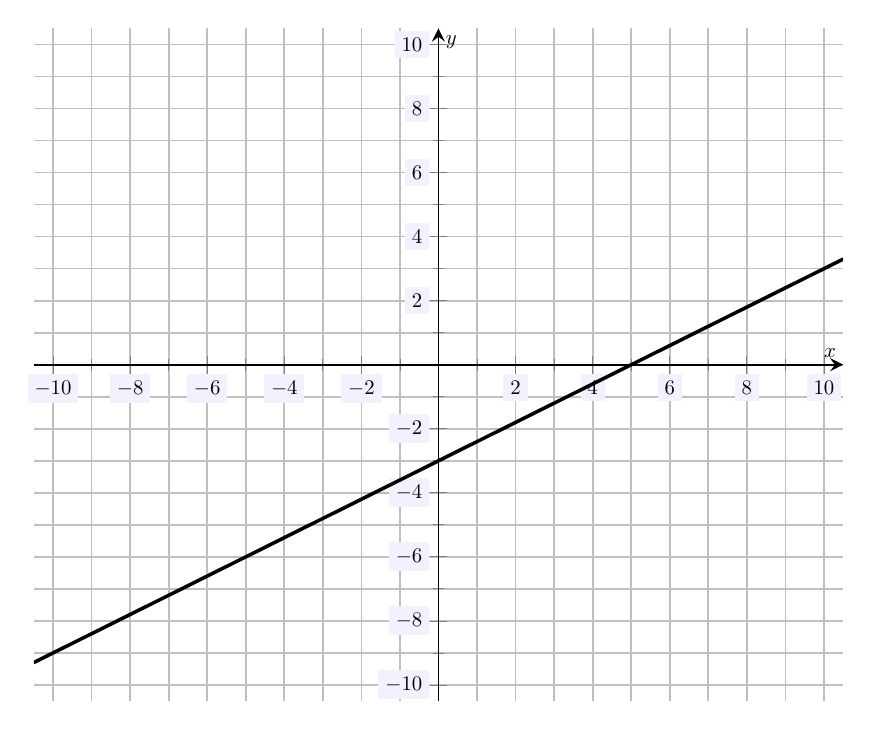
\begin{tikzpicture}[scale=1.5,every node/.style={scale=0.5}]
	\begin{axis}[
	grid=both,
	axis lines=middle,
	ticklabel style={fill=blue!5!white},
	xmin= -10.5, xmax=10.5,
	ymin= -10.5, ymax=10.5,
	xtick={-10,-8,-6,-4,-2,0,2,4,6,8,10},
	ytick={-10,-8,-6,-4,-2,0,2,4,6,8,10},
	minor tick = {-10,-9,...,10},
	xlabel=\(x\),ylabel=\(y\),
	]
	\addplot[domain=-10.5:10.5,samples=2,line width=0.03cm] (x, 3/5*x - 3);
	\end{axis}
	\end{tikzpicture}
	}
	\] \pspace


% Problem
\prob Simplify the following:
	\begin{enumerate}[(a)]
	\item $\sqrt{\dfrac{(x y^2)^3}{x y^{-8}}}$
	\item $\left( \dfrac{x^9 y^{-1} (x y^5)^2}{x^{-1} y} \right)^{-1/2}$
	\item $\left( \sqrt[3]{\dfrac{xy (x^{-3} y^5)^{-2}}{x^{-2} y^5}} \right)^{-2}$
	\end{enumerate} \pspace


% Problem
\prob Showing all your work and explaining your reasoning, answer the following:
	\begin{enumerate}[(a)]
	\item Find the equation of the line through $(-5, 9)$ with slope $-\frac{3}{5}$.
	\item Find the equation of the line through $(0, -4)$ and $(-6, -11)$. 
	\end{enumerate} \pspace


% Problem
\prob You have been saving for a new laptop and printer. You will finally have enough money to purchase them both next month. The laptop costs \$1,899 and the printer costs \$220. Next month, the laptop will go on sale for 5\% less while the printer will be marked up 4\%. The sales tax on the items is 7\%. When you make the purchase of the laptop and printer next month, how much will you pay in total? \pspace


% Problem
\prob For each of the following, describe whether the given dependent variable is a function of the independent variable:
	\begin{enumerate}[(a)]
	\item Independent: the number of days since you purchased your car. \par 
		Dependent: the milage for your car. 
	\item Independent: the number of people in a specific room at noon. \par 
		Dependent: the day of the week.
	\item Independent: the day of the year. \par
		Dependent: the sunrise time. 
	\item Independent: your laptop battery percentage. \par
		Dependent: the time remaining until your laptop runs out of power. 
	\end{enumerate} \pspace


% Problem
\prob Consider the relation plotted below:
	\[
	\fbox{
	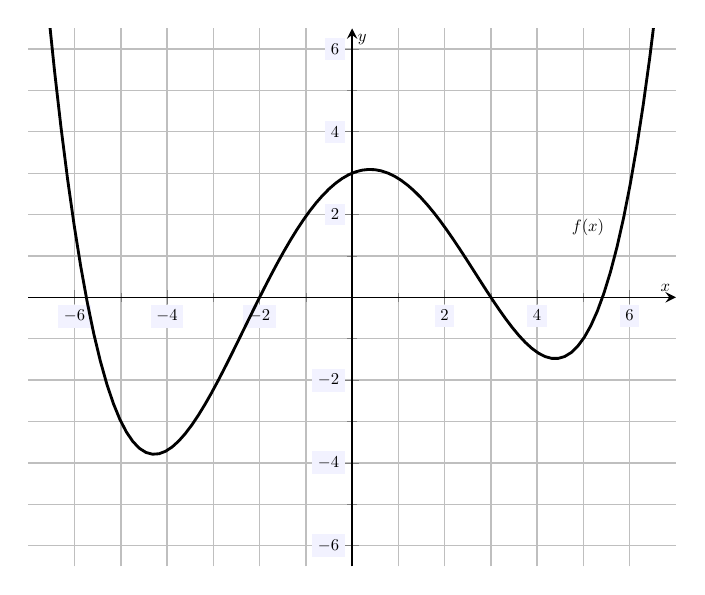
\begin{tikzpicture}[scale=1.2,every node/.style={scale=0.5}]
	\begin{axis}[
	grid=both,
	axis lines=middle,
	ticklabel style={fill=blue!5!white},
	xmin= -7, xmax=7,
	ymin= -6.5, ymax=6.5,
	xtick={-6,-4,-2,0,2,4,6},
	ytick={-6,-4,-2,0,2,4,6},
	minor tick = {-5,-3,...,5},
	xlabel=\(x\),ylabel=\(y\),
	]
	\addplot[domain=-7:7, samples=100,line width=0.03cm] (x,3+0.467857*x-0.601786*x^2-0.0107143*x^3+0.0160714*x^4);
	\node at (5.1,1.7) {$f(x)$};
	\end{axis}
	\end{tikzpicture}
	}
	\]

\begin{enumerate}[(a)]
\item Is the relation, $f(x)$, plotted above a function? Explain. 
\item Find the $y$-intercept.
\item Find the $x$-intercepts. 
\item Find the value of $f(6)$.
\item Find any $x$-values for which $f(x)= 2$.  
\end{enumerate} \pspace


% Problem
\prob Define $f(x)$ to be the relation given by $f(x):= 2.7x + 14.9$.
	\begin{enumerate}[(a)]
	\item Is $f(x)$ a function? Explain.
	\item Find $f(9)$.
	\item Is there an $x_0$ so that $f(x_0)= 20$? If so, find it. If not, explain why. 
	\item Find the $y$-intercept for $f(x)$. 
	\item Find any $x$-intercepts for $f(x)$.
	\end{enumerate} \pspace


% Problem
\prob Let $f(x)$ and $g(x)$ be the functions given by the values in the table below. \par
	\begin{table}[H]
	\centering
	\begin{tabular}{r||rrrrr}
	$x$ & $-2$ & $-1$ & $0$ & $1$ & $2$ \\ \hline
	$f(x)$ & $4$ & $5$ & $-1$ & $6$ & $0$ \\
	$g(x)$ & $3$ & $-2$ & $7$ & $0$ & $-1$
	\end{tabular}
	\end{table} \par
Compute the following:
	\begin{enumerate}[(a)]
	\item $f(-2) - g(1)$ 
	\item $(f + g)(0)$
	\item $(fg)(-1)$
	\item $(f \circ g)(2)$
	\item $(g \circ f)(2)$
	\end{enumerate} \pspace


% Problem 
\prob Consider the function given by $W(t)= 568.1 - 13.4t$. 
	\begin{enumerate}[(a)]
	\item Is $W(t)$ a linear function? Explain.
	\item Find the slope of $W(t)$.
	\item Find the $y$-intercept of $W(t)$.
	\item Find the $x$-intercept of $W(t)$. 
	\item Find a value of $t$ for which $W(t)= 100$. 
	\end{enumerate} \pspace


% Problem
\prob Consider the relation plotted below.
	\[
	\fbox{
	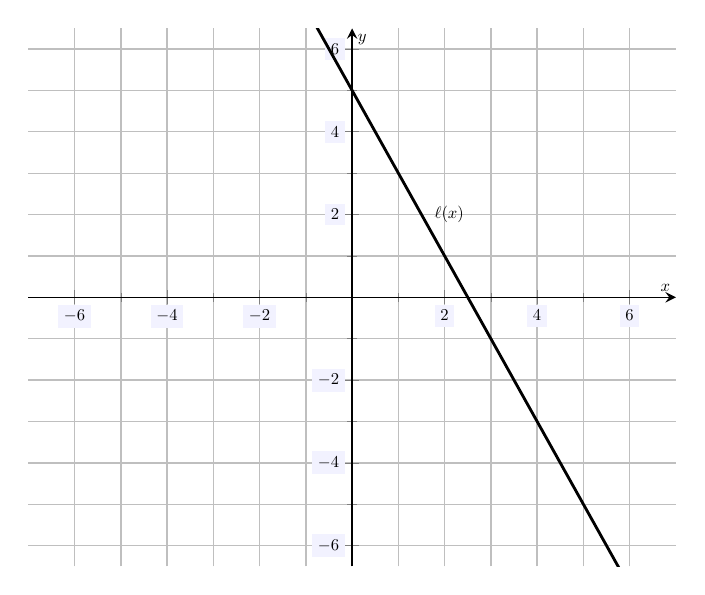
\begin{tikzpicture}[scale=1.2,every node/.style={scale=0.5}]
	\begin{axis}[
	grid=both,
	axis lines=middle,
	ticklabel style={fill=blue!5!white},
	xmin= -7, xmax=7,
	ymin= -6.5, ymax=6.5,
	xtick={-6,-4,-2,0,2,4,6},
	ytick={-6,-4,-2,0,2,4,6},
	minor tick = {-5,-3,...,5},
	xlabel=\(x\),ylabel=\(y\),
	]
	\addplot[domain=-7:7, samples=100,line width=0.03cm] (x,5 - 2*x);
	\node at (2.1,2) {$\ell(x)$};
	\end{axis}
	\end{tikzpicture}
	}
	\]

\begin{enumerate}[(a)]
\item Is $\ell(x)$ a linear function? Explain.
\item Find the equation for $\ell(x)$. 
\item Find the $x$ and $y$-intercepts for $\ell(x)$. 
\item Find a value of $x$ for which $\ell(x)= -3$. 
\end{enumerate} \pspace


% Problem 
\prob Consider the linear function that goes through the points $(-4, 5)$ and $(6, 0)$.
	\begin{enumerate}[(a)]
	\item Find the slope of this linear function.
	\item Find the equation of this linear function.
	\end{enumerate} \pspace


% Problem 
\prob A certain product requires \$800 of upfront costs to produce---the \textit{fixed costs}. After this investment, it costs \$8.50 to produce every item. 
	\begin{enumerate}[(a)]
	\item Explain why the cost to produce $q$ items, $C(q)$, is a linear function.
	\item Find the equation for $C(q)$.
	\item What does the $y$-intercept for $C(q)$ represent?
	\item How much does it cost to produce 10,000~items?
	\item What is the maximum number of items you could produce with \$6,000?
	\end{enumerate} \pspace


% Problem
\prob Showing all your work, simplify the following as much as possible: 
	\[
	\dfrac{x^{-5} y^6}{x^3 y^{-2} (x^3 y^5)^{-2}} \left( \dfrac{xy \big( (x^3 y^{-5})^2 \big)^{-4}}{x^0 y^8 (x^{-5} y^6)^{-12}} \right)^0
	\] \pspace


% Problem
\prob Showing all your work, simplify the following as much as possible: 
	\[
	\sqrt{ \dfrac{9 (a^6 b^5)^{1/3}}{a^{-2} b} }
	\] \pspace


% Problem
\prob Consider the relation $f$ shown below. 
	\[
	\fbox{
	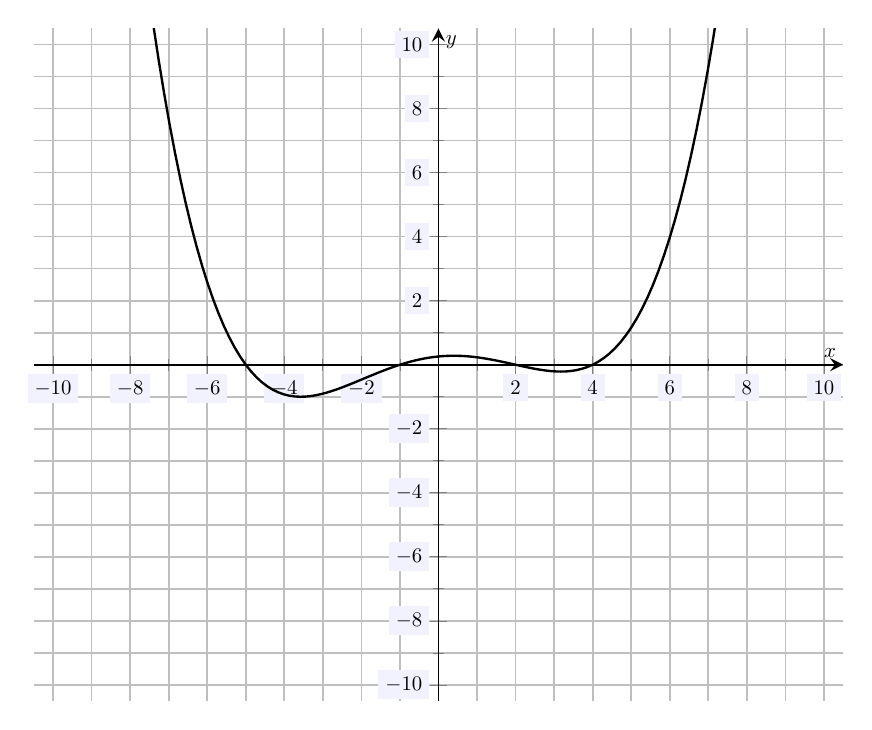
\begin{tikzpicture}[scale=1.5,every node/.style={scale=0.5}]
	\begin{axis}[
	grid=both,
	axis lines=middle,
	ticklabel style={fill=blue!5!white},
	xmin= -10.5, xmax=10.5,
	ymin= -10.5, ymax=10.5,
	xtick={-10,-8,-6,-4,-2,0,2,4,6,8,10},
	ytick={-10,-8,-6,-4,-2,0,2,4,6,8,10},
	minor tick = {-10,-9,...,10},
	xlabel=\(x\),ylabel=\(y\),
	]
	\addplot[line width= 0.02cm,samples=150,domain= -10.5:10.5] ({x},{1/155*(x - 4)*(x - 2)*(x + 1)*(x + 5)});
	\end{axis}
	\end{tikzpicture}
	}
	\] 

\begin{enumerate}[(a)]
\item Is the relation shown above a function of $x$? Explain. 
\item Assuming the relation is a function of $x$, does the relation above have an inverse that is a function of $y$? Explain.
\item Find $f(6)$.
\item Find the $x$-intercepts of $f(x)$.
\item Is there an $x$ such that $f(x)= 2$? Explain. 
\end{enumerate} \pspace


% Problem
\prob Consider the function $\ell(x)= 4x - 6$.
	\begin{enumerate}[(a)]
	\item Is $\ell(x)$ linear? Explain. 
	\item Find the slope and $y$-intercept of $\ell(x)$. 
	\item Compute $\ell(\frac{17}{2})$. 
	\item Is there an $x$ such that $\ell(x)= 10$? Explain. 
	\item Find the $x$-intercept of $\ell(x)$. 
	\end{enumerate} \pspace


% Problem
\prob Find the equation of the line that has $y$-intercept 5 that is parallel to the line shown below. 
	\[
	\fbox{
	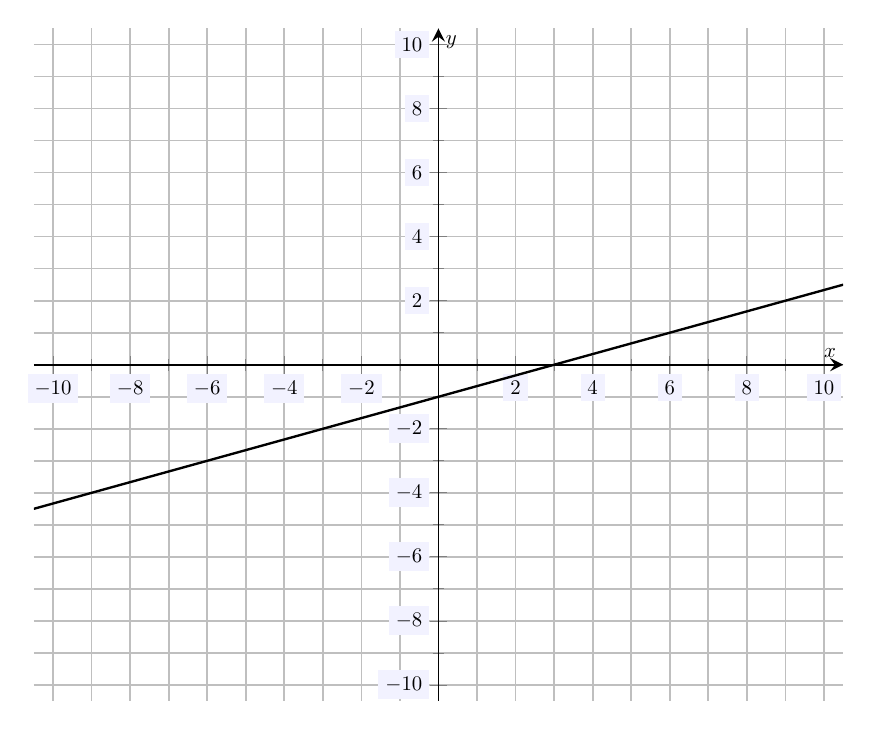
\begin{tikzpicture}[scale=1.5,every node/.style={scale=0.5}]
	\begin{axis}[
	grid=both,
	axis lines=middle,
	ticklabel style={fill=blue!5!white},
	xmin= -10.5, xmax=10.5,
	ymin= -10.5, ymax=10.5,
	xtick={-10,-8,-6,-4,-2,0,2,4,6,8,10},
	ytick={-10,-8,-6,-4,-2,0,2,4,6,8,10},
	minor tick = {-10,-9,...,10},
	xlabel=\(x\),ylabel=\(y\),
	]
	\addplot[line width= 0.02cm,samples=50,domain= -10.5:10.5] ({x},{1/3*x - 1});
	\end{axis}
	\end{tikzpicture}
	}
	\] \pspace


% Problem
\prob Showing all your work, simplify the following as much as possible (express any denominators using negative powers):
	\begin{enumerate}[(a)]
	\item $ab(a^3 b^2)^0$
	\item $x^4 y^9 x^{22} y^5$
	\item $\dfrac{r^0 s^5}{r^4 s^3}$
	\item $(x^8 y^{10}) \left( \dfrac{x^3}{y^8} \right)$
	\item $\dfrac{r^{12} s^4 t^5}{s^3 r^{20} t^5}$
	\end{enumerate} \pspace


% Problem
\prob Showing all your work, simplify the following as much as possible (do not express your answer using any negative powers): 
	\begin{enumerate}[(a)]
	\item $\dfrac{a^6 b^3}{a^{18} b^5}$
	\item $\dfrac{x^6 y^9}{x^{-6} y^{16}}$
	\item $\dfrac{r^{18} s^7 r^{-3} s^{-2}}{ r^{11} s^5}$
	\item $\dfrac{a^0 b^{-5}}{a^{-8} b^7} \cdot \dfrac{b^3}{a^6}$
	\item $\dfrac{x}{y} \left( \dfrac{x^3 y^{-11}}{x^{-5} y^{12}} \cdot \dfrac{x^{-4} y^9}{x^4 y^{-3}} \right)^0$
	\end{enumerate} \pspace


% Problem
\prob Showing all your work, simplify the following as much as possible (do not express your answer using any negative powers): 
	\begin{enumerate}[(a)]
	\item $\big( (x^2 y^3)^3 \big)^3$
	\item $(r^3s)^6 (r^2s^9)^4$	
	\item $(x^{-4} y^6)^{-2} (x^2 y^5)$
	\item $b^6 \left( \dfrac{a^6 b^3}{a^{-3}} \right)^{-4}$
	\item $(xy^2)^{-3} \left( \dfrac{(xy)^2}{xy^{-1}} \right)^{-1}$
	\end{enumerate} \pspace


% Problem
\prob Showing all your work, simplify the following as much as possible:
	\begin{enumerate}[(a)]
	\item $\dfrac{(4x^2)^3 (3x^4)}{(6x^3)^4}$
	\item $\left( - \dfrac{3x^{-2} y^7}{2x^3 y^5} \right)^{-2}$
	\item $\left( \dfrac{x^6 y^3 \cdot (x^5y)^2}{x^{-4} y^{12}} \right)^3$
	\item $\left( \dfrac{x^{r + s}}{x^{2r + 5}} \right)^4$
	\item $(xy)^{-n} \cdot \dfrac{x^{n - 1} y^{m - 1}}{x^{2n} y^n}$
	\end{enumerate} \pspace


% Problem
\prob Determine whether the relations $f(x)= 3x^2 - 4x + 5$ and $g(x, y)= xy^2 - x^2y$ are functions. Be sure to fully justify your answer. Also, find $f(-1)$ and $g(3, -1)$. \pspace


% Problem
\prob Values for several functions are given in the table below. 
        \begin{table}[H]
        \centering
        \begin{tabular}{| c || c | c | c | c | c | c | c |} \hline
	$x$ & $-3$ & $-2$ & $-1$ & $\phantom{-}0$ & $\phantom{-}1$ & $\phantom{-}2$ & $\phantom{-}3$ \\ \hline \hline
	$f(x)$ & $\phantom{-}4$ & $8$ & $-1$ & $\phantom{-}5$ & $-3$ & $\phantom{-}0$ & $-2$ \\ \hline
	$g(x)$ & $\phantom{-}1$ & $6$ & $\phantom{-}0$ & $-6$ & $-7$ & $-3$ & $\phantom{-}1$ \\ \hline
	$h(x)$ & $-4$ & $0$ & $\phantom{-}3$ & $\phantom{-}5$ & $10$ & $\phantom{-}3$ & $\phantom{-}9$ \\ \hline
        \end{tabular}
        \end{table}

Given the data above, compute the following: 
        \begin{enumerate}[(a)]
        \item $(h + g)(-2)=$ 
        \item $(f - g)(0)=$ 
        \item $(5h)(1)=$ 
        \item $\left(\dfrac{h}{f}\right)(1)=$ 
        \item $g(-3)\, h(3)=$ 
        \item $g \big(-1 - f(3) \big)=$ 
        \item $(h \circ g)(2)=$ 
	\item $(g \circ h)(2)=$ 
        \item $(f \circ g)(-1)=$ 
	\item $(h \circ g \circ f)(1)=$ 
        \end{enumerate} \pspace


% Problem
\prob Suppose $f(x)$ and $g(x)$ are the functions given below. 
	\[
	\begin{aligned}
	f(x)&= 2x - 3 \\[0.3cm]
	g(x)&= x^2 + 2x - 1
	\end{aligned}
	\]

Compute the following: \pspace
        \begin{enumerate}[(a)]
        \item $f(5)=$ 
        \item $g(-2)=$ 
        \item $f(0) - 3g(2)=$ 
        \item $(f - g)(x)=$ 
        \item $(fg)(x)=$ 
        \item $\left( \dfrac{f}{g} \right)(x)=$ 
        \item $(f \circ g)(0)=$ 
        \item $(g \circ f)(0)=$ 
        \item $(f \circ g)(x)=$ 
        \item $(g \circ f)(x)=$ 
        \end{enumerate} \pspace


% Problem 
\prob Let $f(x)$ be the function given by $f(x)= 3x - 7$. 
	\begin{enumerate}[(a)]
	\item Find a value in the range of $f$. Be sure to justify why the value is in the range. 
	\item Compute $f(4)$. Is $(4, 1)$ on the graph of $f$? Explain. 
	\item Is there an $x$ such that $f(x)= 11$? Explain. 
	\item Is $1 \in f^{-1}(3)$? Explain. 
	\item Assuming $f^{-1}$ exists, what is $f(f^{-1}(\pi))$ and $f^{-1}(f(\sqrt{2}))$?
	\end{enumerate} \pspace


% Problem
\prob Find the equation of the line plotted below.
	\[
	\fbox{
	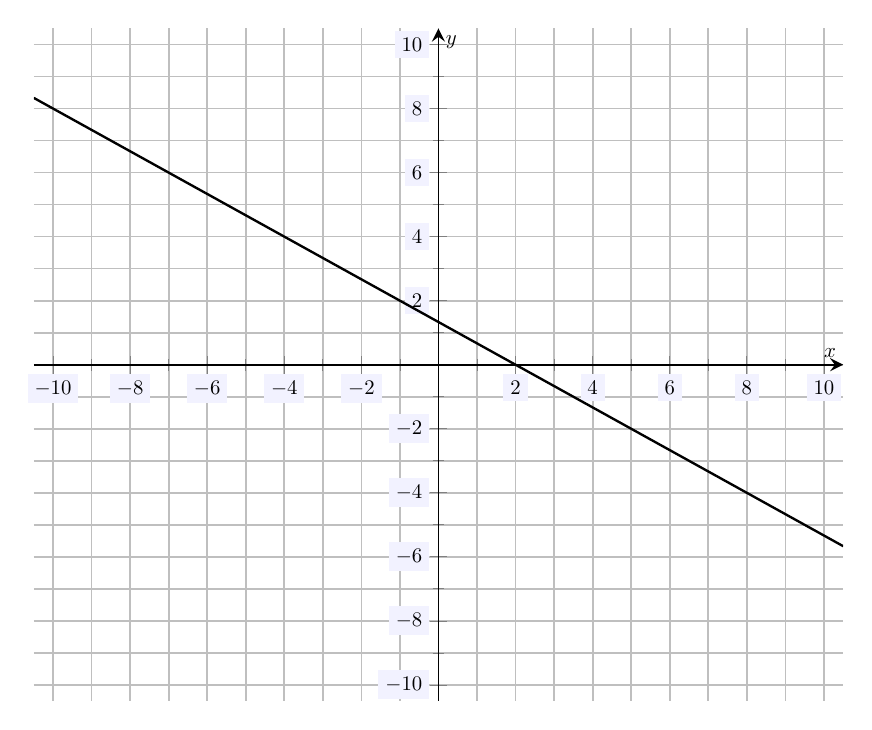
\begin{tikzpicture}[scale=1.5,every node/.style={scale=0.5}]
	\begin{axis}[
	grid=both,
	axis lines=middle,
	ticklabel style={fill=blue!5!white},
	xmin= -10.5, xmax=10.5,
	ymin= -10.5, ymax=10.5,
	xtick={-10,-8,-6,-4,-2,0,2,4,6,8,10},
	ytick={-10,-8,-6,-4,-2,0,2,4,6,8,10},
	minor tick = {-10,-9,...,10},
	xlabel=\(x\),ylabel=\(y\),
	]
	\addplot[line width= 0.02cm,samples=2,domain= -10.5:10.5] ({x},{4/3 - 2/3*x});
	\end{axis}
	\end{tikzpicture}
	}
	\] \pspace


% Problem
\prob Find the equation of the line containing the point $(-5, 6)$ with slope $-\frac{1}{3}$. \pspace


% Problem
\prob Find the equation of the line with $x$-intercept 5 and $y$-intercept $-6$. \pspace


% Problem
\prob Consider the linear function $\ell(x)= \frac{13 - 11x}{5}$. 
	\begin{enumerate}[(a)]
	\item Find the slope of this function.
	\item Find the $y$-intercept of this function.
	\item Find the $x$-intercept of this function.
	\item Does the graph of this function contain the point $(6, -8)$? Explain. 
	\end{enumerate} \pspace


% Problem
\prob Solve the following equation and verify that your solution is correct:
	\[
	9 - 3(x + 1)= \dfrac{6 - x}{2}
	\] \pspace


% Problem
\prob Find the equation of the line perpendicular to the line $y= \pi$ with $x$-intercept $\sqrt{2}$. \pspace 


% Problem
\prob Find the inverse of the linear function $\ell(x)= \frac{5}{6} - 8x$. Use this inverse function to solve the equation $\ell(x)= 10$. \pspace


% Problem
\prob Find the line perpendicular to the line $y= 7 - \frac{2}{3}x$ that contains the $x$-intercept of the line $y= 7x + 3$. \pspace


% Problem
\prob Showing all your work, simplify the following as much as possible (express any denominators using negative powers):
	\begin{enumerate}[(a)]
	\item $\dfrac{x^5 y^3}{x^3 y^9}$
	\item $\dfrac{(x^2 y^{-3})^4}{x^0 y^2}$
	\item $\dfrac{(x^8 y^3)^0 x y^7}{(x^2)^3 y}$
	\end{enumerate} \pspace


% Problem
\prob Showing all your work, simplify the following as much as possible (do not express your answer using any negative powers): 
	\begin{enumerate}[(a)]
	\item $\dfrac{x^{-2} y z^6}{x y^{-6} z^5}$
	\item $\dfrac{(x y^{-2})^{-1}}{x^3 y^{-7}}$
	\item $\left( \dfrac{x^5 y^{-4}}{(x^{-4} y^3)^{-8}} \right)^0$
	\end{enumerate} \pspace


% Problem
\prob Showing all your work, simplify the following as much as possible (do not express your answer using any negative powers): 
	\[
	\dfrac{\left( (x y z)^5 x z^{-4} \right)^2 x^{-5}}{x y^{-3} z^{-2}}
	\] \pspace





\newpage





% Problem
\prob Simplify the following:
	\begin{enumerate}[(a)]
	\item $\sqrt{x^{10} y^4}$
	\item $\sqrt[3]{x^3 y^5 z^{12}}$
	\item $\sqrt{\sqrt[3]{y^6}}$
	\end{enumerate} \pspace  	


% Problem
\prob Simplify the following:
	\begin{enumerate}[(a)]
	\item $x^2 y \sqrt{x^8 y^5}$
	\item $\dfrac{x^2 y}{\sqrt[3]{x y^6}}$
	\item $\dfrac{\sqrt{x^2 y}}{\sqrt[3]{x^3 y^5}}$
	\end{enumerate} \pspace  


% Problem
\prob Simplify the following:
	\[
	\left( \dfrac{\sqrt{x^8 y^6}}{x^{-3} \sqrt{x y}} \right)^{-3/2}
	\] \pspace



% Problem
\prob Determine whether the relations $F$ and $G$ shown below are functions. Be sure to fully justify your answer. \pspace
	\hfill
	\begin{minipage}[c]{0.48\textwidth}
	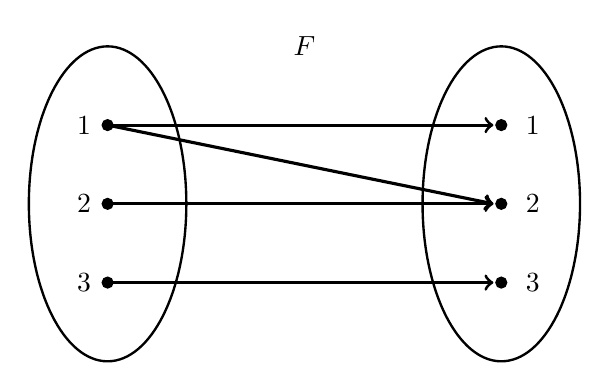
\begin{tikzpicture}
	\node at (2.5,2) {$F$};
	% Ellipses
	\draw[line width=0.03cm] (0,0) circle (1 and 2);
	\draw[line width=0.03cm] (5,0) circle (1 and 2);
	
	% Nodes
	\draw[fill=black] (0,1) circle (0.07);
	\draw[fill=black] (0,0) circle (0.07);
	\draw[fill=black] (0,-1) circle (0.07);
	
	\draw[fill=black] (5,1) circle (0.07);
	\draw[fill=black] (5,0) circle (0.07);
	\draw[fill=black] (5,-1) circle (0.07);
	
	% Arrow
	\draw[line width=0.04cm,->] (0,1) -- (4.9,1);
	\draw[line width=0.04cm,->] (0,1) -- (4.9,0);
	\draw[line width=0.04cm,->] (0,0) -- (4.9,0);
	\draw[line width=0.04cm,->] (0,-1) -- (4.9,-1);
	
	% Labels
	\node at (-0.3,1) {$1$};
	\node at (-0.3,0) {$2$};
	\node at (-0.3,-1) {$3$};
	
	\node at (5.4,1) {$1$};
	\node at (5.4,0) {$2$};
	\node at (5.4,-1) {$3$};
	\end{tikzpicture}
	\end{minipage}%
	\begin{minipage}[c]{0.40\textwidth}
	\begin{table}[H]
	\centering
	\begin{tabular}{cc}
	$x$ & $G$ \\ \hline
	$1$ & $1$ \\
	$2$ & $1$ \\
	$3$ & $1$ \\
	$4$ & $1$ \\
	$5$ & $1$
	\end{tabular}
	\end{table}
	\end{minipage} \pspace


% Problem
\prob Determine whether the relations $f(x)= 16 - x^2$ and $g(x, y)= \dfrac{x + y}{x - y}$ are functions. Be sure to fully justify your answer. Also, find $f(5)$ and $g(4, 5)$. \pspace


% Problem
\prob Suppose $f(x)$ and $g(x)$ are the functions given below. 
	\[
	\begin{aligned}
	f(x)&= 1 - 4x \\[0.3cm]
	g(x)&= x^2 + 1
	\end{aligned}
	\]

Compute the following: \pspace
        \begin{enumerate}[(a)]
        \item $6f(1) - g(2)$ 
        \item $(f + g)(1)$ 
        \item $(f - g)(0)$ 
        \item $(fg)(2)$ 
        \item $(f \circ g)(-1)$ 
        \item $(g \circ f)(-1)$ 
        \end{enumerate} \pspace


% Problem
\prob Let $f(x)$ be the function given by $f(x)= 4x - 5$. 
	\begin{enumerate}[(a)]
	\item Find a value in the range of $f$. Be sure to justify why the value is in the range. 
	\item Compute $f(-1)$. Is $(-1, -9)$ on the graph of $f$? Explain. 
	\item Is there an $x$ such that $f(x)= 11$? Explain. 
	\item Is $2 \in f^{-1}(0)$? Explain. 
	\item Assuming $f^{-1}$ exists, what is $f(f^{-1}(\sqrt{2}))$ and $f^{-1}(f(\sqrt{2}))$?
	\end{enumerate} \pspace


% Problem
\prob Consider the relation $f$ plotted below. 
	\[
	\fbox{
	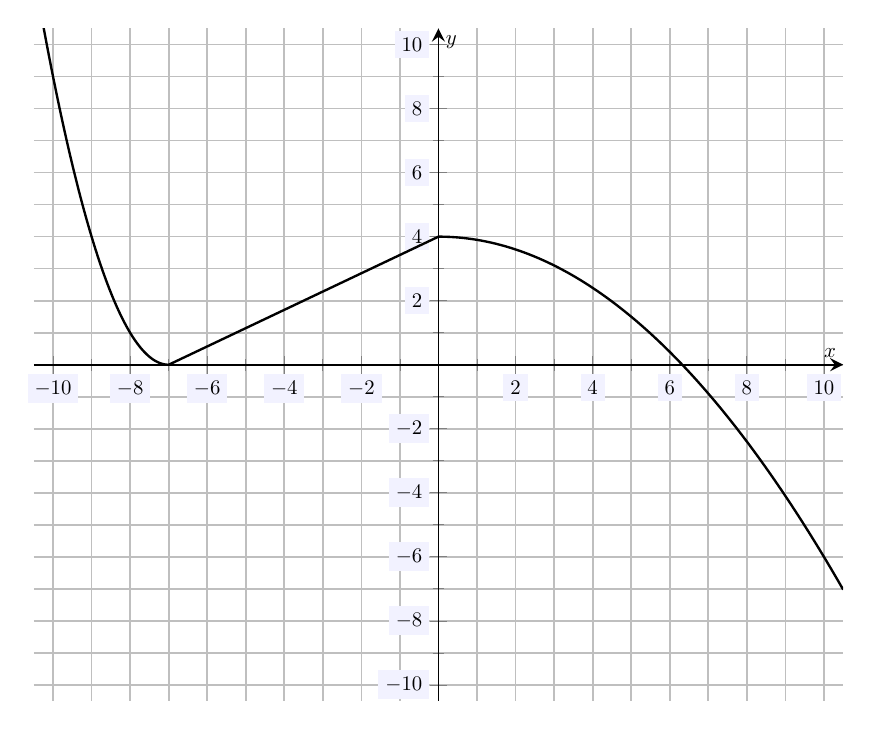
\begin{tikzpicture}[scale=1.5,every node/.style={scale=0.5}]
	\begin{axis}[
	grid=both,
	axis lines=middle,
	ticklabel style={fill=blue!5!white},
	xmin= -10.5, xmax=10.5,
	ymin= -10.5, ymax=10.5,
	xtick={-10,-8,-6,-4,-2,0,2,4,6,8,10},
	ytick={-10,-8,-6,-4,-2,0,2,4,6,8,10},
	minor tick = {-10,-9,...,10},
	xlabel=\(x\),ylabel=\(y\),
	]
	\addplot[line width= 0.02cm,samples=100,domain= -10.5:-7] ({x},{(x + 7)^2}); 
	\addplot[line width= 0.02cm,samples=100,domain= -7:0] ({x},{4/7*x + 4}); 
	\addplot[line width= 0.02cm,samples=100,domain= 0:10.5] ({x},{-x^2/10 + 4}); 
	\end{axis}
	\end{tikzpicture}
	}
	\] 

\begin{enumerate}[(a)]
\item Compute $f(-9)$ and $f(10)$. 
\item Is $f(x)$ a function? Explain. 
\item Does $f(x)$ have an inverse? If so, sketch the inverse. If not, explain why. 
\end{enumerate} \pspace


% Problem
\prob Showing all your work, verify that $g(x)= \frac{1 - x}{5}$ is the inverse function for $f(x)= 1 - 5x$. Also, compute $g(6)$. What does the value of $g(6)$ tell you about the function $f(x)$? \pspace


% Problem
\prob Consider the function $\ell(x)= 5x + 2$.
        \begin{enumerate}[(a)]
        \item What is the graph of the function $\ell(x)$.
        \item Find two points on the graph of $\ell(x)$.
        \item Is the point $(2, 5)$ on the graph of $\ell(x)$? Explain. 
        \item Is the point $(-1, -3)$ on the graph of $\ell(x)$? Explain. 
        \end{enumerate} \pspace


% Problem
\prob A relation $\phi$ is plotted below. 
	\[
	\fbox{
	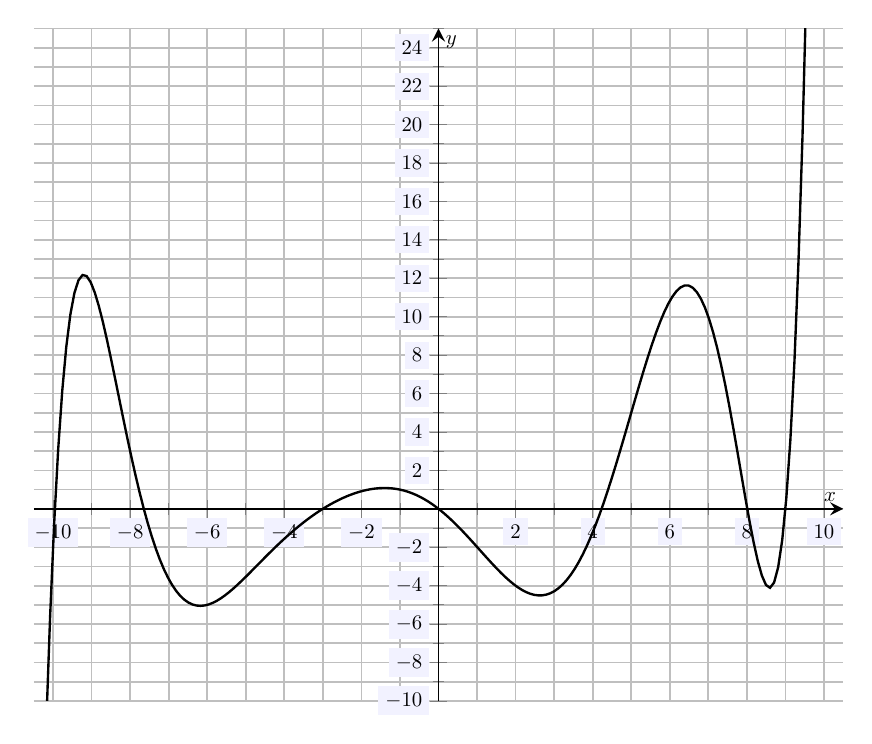
\begin{tikzpicture}[scale=1.5,every node/.style={scale=0.5}]
	\begin{axis}[
	grid=both,
	axis lines=middle,
	ticklabel style={fill=blue!5!white},
	xmin= -10.5, xmax=10.5,
	ymin= -10, ymax=25,
	xtick={-10,-8,-6,-4,-2,0,2,4,6,8,10},
	ytick={-10,-8,...,25},
	minor tick = {-10,-9,...,25},
	xlabel=\(x\),ylabel=\(y\),
	]
	\addplot[line width= 0.02cm,samples=200,domain= -10.5:10.5] ({x},{-1.56755*x - 0.529734*x^2 + 0.0728113*x^3 + 0.039114*x^4 +  0.00344758*x^5 - 0.000794827*x^6 - 0.000120631*x^7 + 0.00000498369*x^8 + 0.000000848123*x^9}); 
	\end{axis}
	\end{tikzpicture}
	}
	\] 
Using the plot above, answer the following:
	\begin{enumerate}[(a)]
	\item Compute $\phi(5)$.
	\item Find the $y$-intercept for $\phi(x)$. 
	\item Find the $x$-intercepts for $\phi(x)$. 	
	\item As accurately as possible, compute the preimage of $-5$, i.e. $\phi^{-1}(-5)$. 
	\item Explain why (d) implies that $\phi$ does not have an inverse function. 
	\end{enumerate} \pspace


% Problem
\prob Find the equation of the horizontal line through $(0, -2)$. \pspace


% Problem
\prob Find the equation of the line parallel to the line $y= 6 - x$ containing the point $(-6, 1)$. \pspace


% Problem
\prob Find the equation of the line perpendicular to the line $y= \frac{5}{3} x + 1$ passing through the point $(10, -13)$. \pspace


% Problem
\prob Solve the following equation and verify that your solution is correct:
	\[
	-2(5 - x) + 15= \dfrac{8x + 1}{2}
	\] \pspace


% Problem
\prob Solve the following equation:
	\[
	\sqrt{2}\, (x - \sqrt{8})= \pi x + 5
	\] \pspace


% Problem
\prob Find the equation of the line plotted below.
	\[
	\fbox{
	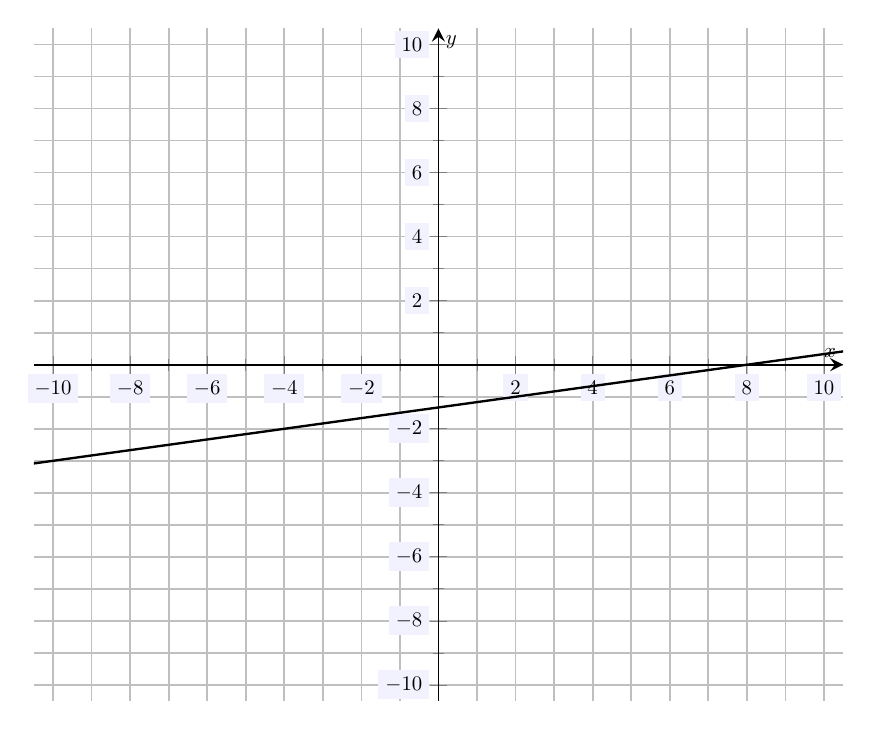
\begin{tikzpicture}[scale=1.5,every node/.style={scale=0.5}]
	\begin{axis}[
	grid=both,
	axis lines=middle,
	ticklabel style={fill=blue!5!white},
	xmin= -10.5, xmax=10.5,
	ymin= -10.5, ymax=10.5,
	xtick={-10,-8,-6,-4,-2,0,2,4,6,8,10},
	ytick={-10,-8,-6,-4,-2,0,2,4,6,8,10},
	minor tick = {-10,-9,...,10},
	xlabel=\(x\),ylabel=\(y\),
	]
	\addplot[line width= 0.02cm,samples=2,domain= -10.5:10.5] ({x},{-4/3 + 1/6*x});
	\end{axis}
	\end{tikzpicture}
	}
	\] \pspace


% Problem
\prob Find the equation of the following lines:
	\begin{enumerate}[(a)]
	\item The line through $(-1, 1)$ and $(6, -2)$.
	\item The line containing $(8, -1)$ with slope $\frac{4}{3}$.
	\item The line with $y$-intercept 5 and slope $-6$.
	\end{enumerate} \pspace


% Problem
\prob Find the equation of the line with $x$-intercept $-4$ and $y$-intercept $6$. \pspace


% Problem
\prob Consider the linear function $\ell(x)= \dfrac{5x - 7}{-3}$. 
	\begin{enumerate}[(a)]
	\item Find the slope of this function.
	\item Find the $y$-intercept of this function.
	\item Find the $x$-intercept of this function.
	\item Does the graph of this function contain the point $(2, 0)$? Explain. 
	\end{enumerate} \pspace


% Problem
\prob Find the $x$-intercept of the line perpendicular to the line $y= \frac{2}{3}x + 5$ that contains the point $(-1, 6)$. \pspace


% Problem
\prob Find the inverse of the linear function $\ell(x)= 6x - 1$. Use this inverse function to solve the equation $\ell(x)= 10$. \pspace


% Problem
\prob Explain why the lines $\ell_1(x)= 5x - 1$ and $\ell_2(x)= 2 - 3x$ intersect. Find their point of intersection. \pspace


% Problem
\prob Find the $x$ and $y$-intercept for the line $y= \dfrac{6x - 11}{3}$. \pspace


% Problem
\prob Let $\ell(x)$ be the linear function given by $\ell(x)= 5x + c$, where $c$ is some constant. Find the value of $c$ such that $\ell(x)$ contains the point $(5, -4)$. What is the $x$-intercept of this line? \pspace


% Problem
\prob Simplify the following, being sure to have no negative exponents in your expression. \pspace
\begin{enumerate}[(a)]
\item $\dfrac{x^{-6}}{x^{-3}}=$ 
\item $\dfrac{(xy^2)^2}{x^2 y^3}=$ 
\item $\dfrac{x^6 y^{-3}}{x^3 y^2}=$ 
\item $\left( \dfrac{y^3}{x^2} \right)^{-2}=$ 
\end{enumerate} \pspace


% Problem
\prob Consider the following relations below:

	\[
	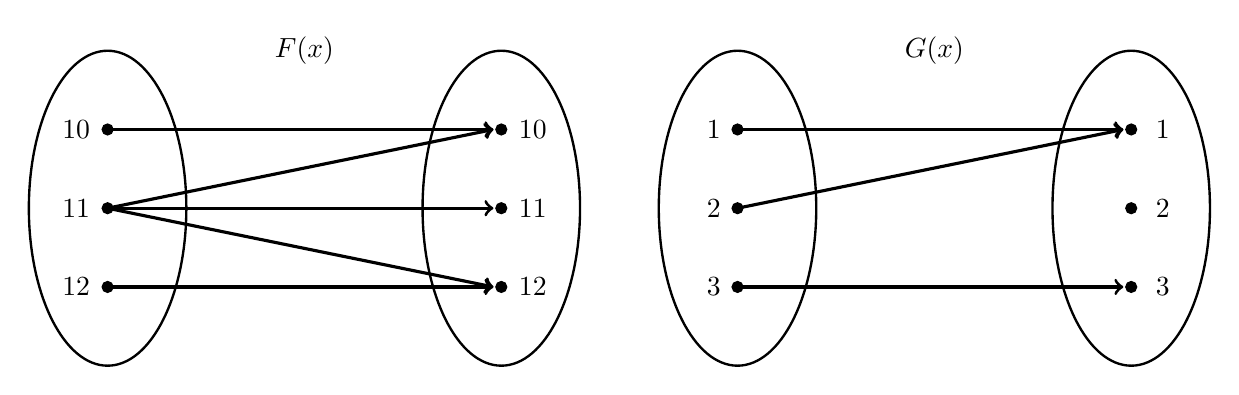
\begin{tikzpicture}
	\node at (2.5,2) {$F(x)$};
	
	% Ellipses
	\draw[line width=0.03cm] (0,0) circle (1 and 2);
	\draw[line width=0.03cm] (5,0) circle (1 and 2);
	
	% Nodes
	\draw[fill=black] (0,1) circle (0.07);
	\draw[fill=black] (0,0) circle (0.07);
	\draw[fill=black] (0,-1) circle (0.07);
	
	\draw[fill=black] (5,1) circle (0.07);
	\draw[fill=black] (5,0) circle (0.07);
	\draw[fill=black] (5,-1) circle (0.07);
	
	% Arrow
	\draw[line width=0.04cm,->] (0,1) -- (4.9,1);
	\draw[line width=0.04cm,->] (0,0) -- (4.9,1);
	\draw[line width=0.04cm,->] (0,0) -- (4.9,0);
	\draw[line width=0.04cm,->] (0,0) -- (4.9,-1);
	\draw[line width=0.04cm,->] (0,-1) -- (4.9,-1);
	
	% Labels
	\node at (-0.4,1) {$10$};
	\node at (-0.4,0) {$11$};
	\node at (-0.4,-1) {$12$};
	
	\node at (5.4,1) {$10$};
	\node at (5.4,0) {$11$};
	\node at (5.4,-1) {$12$};
	
	%
	\tikzset{shift={(8,0)}}	
	
	\node at (2.5,2) {$G(x)$};
	
	% Ellipses
	\draw[line width=0.03cm] (0,0) circle (1 and 2);
	\draw[line width=0.03cm] (5,0) circle (1 and 2);
	
	% Nodes
	\draw[fill=black] (0,1) circle (0.07);
	\draw[fill=black] (0,0) circle (0.07);
	\draw[fill=black] (0,-1) circle (0.07);
	
	\draw[fill=black] (5,1) circle (0.07);
	\draw[fill=black] (5,0) circle (0.07);
	\draw[fill=black] (5,-1) circle (0.07);
	
	% Arrow
	\draw[line width=0.04cm,->] (0,1) -- (4.9,1);
	\draw[line width=0.04cm,->] (0,0) -- (4.9,1);
	\draw[line width=0.04cm,->] (0,-1) -- (4.9,-1);
	
	% Labels
	\node at (-0.3,1) {$1$};
	\node at (-0.3,0) {$2$};
	\node at (-0.3,-1) {$3$};
	
	\node at (5.4,1) {$1$};
	\node at (5.4,0) {$2$};
	\node at (5.4,-1) {$3$};
	\end{tikzpicture}
	\] \pspace

	\begin{minipage}[b]{0.49\textwidth}
	\centering
	\begin{tabular}{c|rcc|r}
	$x$ & $H(x)$ & \hspace{1cm} & $x$ & $J(x)$ \\ \cline{1-2} \cline{4-5}
	$1$ & $1$ & & $5$ & $-1$ \\
	$2$ & $2$ & & $6$ & $-2$ \\
	$3$ & $3$ & & $7$ & $-3$ \\
	$4$ & $4$ & & $8$ & $-4$ \\
	$1$ & $5$ & & $9$ & $-6$
	\end{tabular}
	\end{minipage}
	\begin{minipage}[b]{0.49\textwidth}
	\[
	\begin{aligned}
	K(x)&:= 0.782x - 1283 \\[0.6cm]
	L(x)&:= 2x(x^2 + 1)(x^4 + 1)
	\end{aligned}
	\]
	\end{minipage} \pvspace{0.6cm}
	
Determine if each of the relations given above is a function. \pspace


% Problem
\prob Determine if the relations $f(x)$ and $g(x)$ shown below are functions. Explain why or why not. 
	\[
	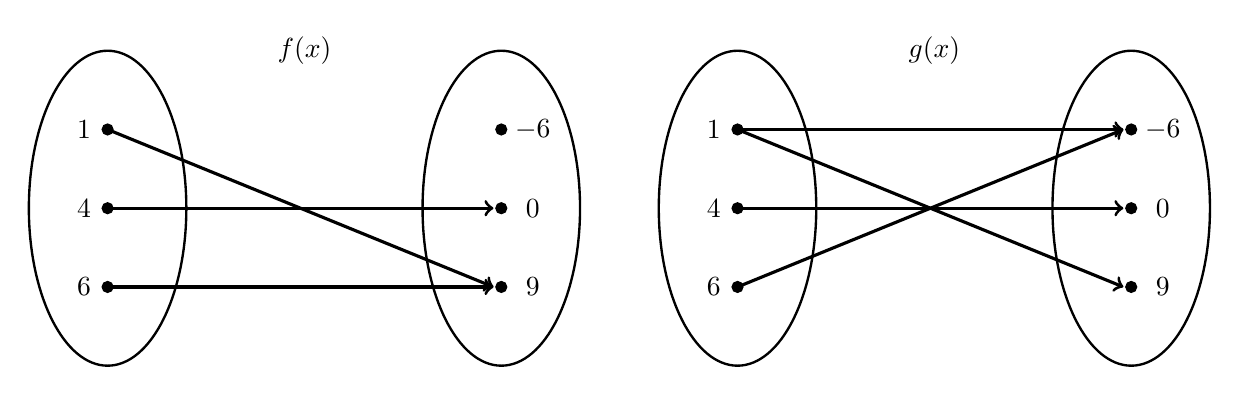
\begin{tikzpicture}
	\node at (2.5,2) {$f(x)$};
	% Ellipses
	\draw[line width=0.03cm] (0,0) circle (1 and 2);
	\draw[line width=0.03cm] (5,0) circle (1 and 2);
	
	% Nodes
	\draw[fill=black] (0,1) circle (0.07);
	\draw[fill=black] (0,0) circle (0.07);
	\draw[fill=black] (0,-1) circle (0.07);
	
	\draw[fill=black] (5,1) circle (0.07);
	\draw[fill=black] (5,0) circle (0.07);
	\draw[fill=black] (5,-1) circle (0.07);
	
	% Arrow
	\draw[line width=0.04cm,->] (0,1) -- (4.9,-1);
	\draw[line width=0.04cm,->] (0,0) -- (4.9,0);
	\draw[line width=0.04cm,->] (0,-1) -- (4.9,-1);
	
	% Labels
	\node at (-0.3,1) {$1$};
	\node at (-0.3,0) {$4$};
	\node at (-0.3,-1) {$6$};
	
	\node at (5.4,1) {$-6$};
	\node at (5.4,0) {$0$};
	\node at (5.4,-1) {$9$};
	
	\tikzset{shift={(8,0)}}
	%
	\node at (2.5,2) {$g(x)$};
	% Ellipses
	\draw[line width=0.03cm] (0,0) circle (1 and 2);
	\draw[line width=0.03cm] (5,0) circle (1 and 2);
	
	% Nodes
	\draw[fill=black] (0,1) circle (0.07);
	\draw[fill=black] (0,0) circle (0.07);
	\draw[fill=black] (0,-1) circle (0.07);
	
	\draw[fill=black] (5,1) circle (0.07);
	\draw[fill=black] (5,0) circle (0.07);
	\draw[fill=black] (5,-1) circle (0.07);
	
	% Arrow
	\draw[line width=0.04cm,->] (0,1) -- (4.9,-1);
	\draw[line width=0.04cm,->] (0,1) -- (4.9,1);
	\draw[line width=0.04cm,->] (0,0) -- (4.9,0);
	\draw[line width=0.04cm,->] (0,-1) -- (4.9,1);
	
	% Labels
	\node at (-0.3,1) {$1$};
	\node at (-0.3,0) {$4$};
	\node at (-0.3,-1) {$6$};
	
	\node at (5.4,1) {$-6$};
	\node at (5.4,0) {$0$};
	\node at (5.4,-1) {$9$};
	\end{tikzpicture}
	\] \pspace


% Problem
\prob Determine if the relations $f(x)$ and $g(x)$ shown below are functions. Explain why or why not. 
	\begin{table}[H]
	\centering
	\begin{tabular}{c|rcc|r}
	$x$ & $f(x)$ & \hspace{1cm} & $x$ & $g(x)$ \\ \cline{1-2} \cline{4-5}
	$1$ & $5$ & & $5$ & $2$ \\
	$2$ & $-5$ & & $6$ & $e$ \\
	$3$ & $4$ & & $8$ & $-3$ \\
	$4$ & $1$ & & $9$ & $2.43$ \\
	$5$ & $0$ & & $5$ & $1$
	\end{tabular}
	\end{table} \pspace


% Problem
\prob Determine if the relations $f(x)$ and $g(x)$ shown below are functions. Explain why or why not. 
	\[
	\begin{aligned}
	f(x)&= 9.87x + 10 \\[0.3cm]
	g(x)&= x^2 - x + 1
	\end{aligned}
	\] \pspace


% Problem
\prob Suppose $f(x)$ is the function given below.
	\[
	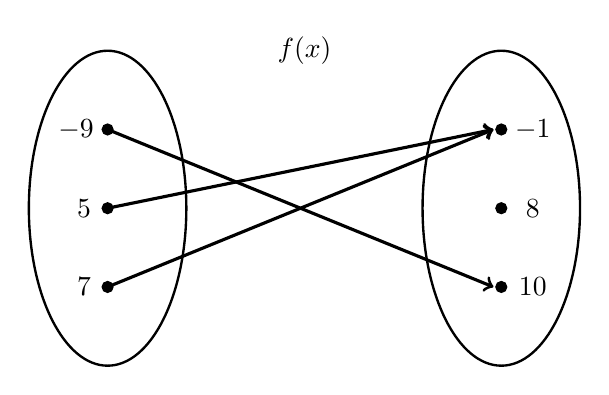
\begin{tikzpicture}
	\node at (2.5,2) {$f(x)$};
	% Ellipses
	\draw[line width=0.03cm] (0,0) circle (1 and 2);
	\draw[line width=0.03cm] (5,0) circle (1 and 2);
	
	% Nodes
	\draw[fill=black] (0,1) circle (0.07);
	\draw[fill=black] (0,0) circle (0.07);
	\draw[fill=black] (0,-1) circle (0.07);
	
	\draw[fill=black] (5,1) circle (0.07);
	\draw[fill=black] (5,0) circle (0.07);
	\draw[fill=black] (5,-1) circle (0.07);
	
	% Arrow
	\draw[line width=0.04cm,->] (0,1) -- (4.9,-1);
	\draw[line width=0.04cm,->] (0,0) -- (4.9,1);
	\draw[line width=0.04cm,->] (0,-1) -- (4.9,1);
	
	% Labels
	\node at (-0.4,1) {$-9$};
	\node at (-0.3,0) {$5$};
	\node at (-0.3,-1) {$7$};
	
	\node at (5.4,1) {$-1$};
	\node at (5.4,0) {$8$};
	\node at (5.4,-1) {$10$};
	\end{tikzpicture}
	\]

\begin{enumerate}[(a)]
\item What is the domain of $f(x)$?
\item What is the codomain of $f(x)$?
\item What is the range of $f(x)$?
\end{enumerate} \pspace


% Problem
\prob Suppose $f(x)$ and $g(x)$ are the functions given below. 
        \begin{table}[H]
        \centering
        \begin{tabular}{| c || c | c | c | c | c | c | c |} \hline
	$x$ & $-2$ & $0$ & $1$ & $3$ & $4$ & $5$ & $10$ \\ \hline
	$f(x)$ & $-1$ & $-7$ & $5$ & $-2$ & $\pi$ & $19$ & $10$ \\ \hline
	$g(x)$ & $17$ & $1$ & $12$ & $0$ & $4$ & $8$ & $6$ \\ \hline
        \end{tabular}
        \end{table} \par
Compute the following: \pspace
        \begin{enumerate}[(a)]
        \item $f(1)=$ 
        \item $g(0)=$ 
        \item $(f + g)(5)=$ 
        \item $(f - g)(-2)=$ 
        \item $(6f)(1)=$ 
        \item $\left(\dfrac{f}{g}\right)(10)=$ 
        \item $f(4)\, g(5)=$ 
        \item $f(2 + g(0))=$ 
        \item $(f \circ g)(0)=$ 
        \item $(g \circ f)(3)=$ 
        \end{enumerate} \pspace


% Problem
\prob Suppose $f(x)$ and $g(x)$ are the functions given below. 
	\[
	\begin{aligned}
	f(x)&= 5x - 1 \\[0.3cm]
	g(x)&= x^2 + 2x + 3
	\end{aligned}
	\]

Compute the following: \pspace
\begin{enumerate}[(a)]
\item $f(1)=$ 
\item $g(0)=$ 
\item $f(1) - 2g(1)=$ 
\item $f(x) - g(x)=$ 
\item $f(x) \, g(x)=$ 
\item $\left( \dfrac{f}{g} \right)(x)=$ 
\item $(g \circ f)(1)=$ 
\item $f(g(0))=$ 
\item $(f \circ g)(x)=$ 
\item $(g \circ f)(x)=$ 
\end{enumerate} \pspace


% Problem
\prob Do the points $(5, 2)$, $(1, -1)$, and $(-3, 4)$ lie along a line? Explain. \pspace


% Problem
\prob Consider the line given by the function $\ell(x)= 1 - 3x$.
        \begin{enumerate}[(a)]
        \item Write this line in the form $Ax + By= C$ for some $A, B, C$. 
        \item What is the slope of this line?
        \item Find the $y$-intercept of the line.
        \item Find the $x$-intercept of the line. 
        \end{enumerate} \pspace


% Problem
\prob Find the equation of the line plotted below.
	\[
	\fbox{
	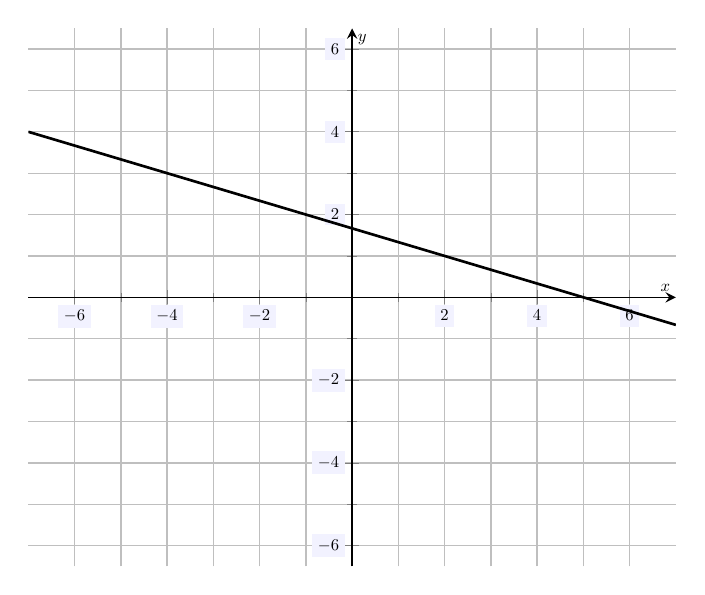
\begin{tikzpicture}[scale=1.2,every node/.style={scale=0.5}]
	\begin{axis}[
	grid=both,
	axis lines=middle,
	ticklabel style={fill=blue!5!white},
	xmin= -7, xmax=7,
	ymin= -6.5, ymax=6.5,
	xtick={-6,-4,-2,0,2,4,6},
	ytick={-6,-4,-2,0,2,4,6},
	minor tick = {-5,-3,...,5},
	xlabel=\(x\),ylabel=\(y\),
	]
	\addplot[thick, domain= -7:7] {-1/3*x + 5/3};
	\end{axis}
	\end{tikzpicture}
	}
	\] \pspace


% Problem
\prob Find the equation of the line through the point $(3, -1)$ with slope $-2$. \pspace


% Problem
\prob Find the equation of the line through $(-2, 2)$ and $(3, 4)$. \pspace


% Problem
\prob Find the equation of the line perpendicular to the line $y= 6$ that contains the point $(-3, 9)$. \pspace


% Problem
\prob Find the equation of the line that is perpendicular to the line $y= 7x - 1$ that passes through the $x$-intercept of the line $y= 4x - 8$. \pspace


% Problem
\prob Determine if the relations $f(x)$ and $g(x)$ shown below are functions. Explain why or why not. 
	\[
	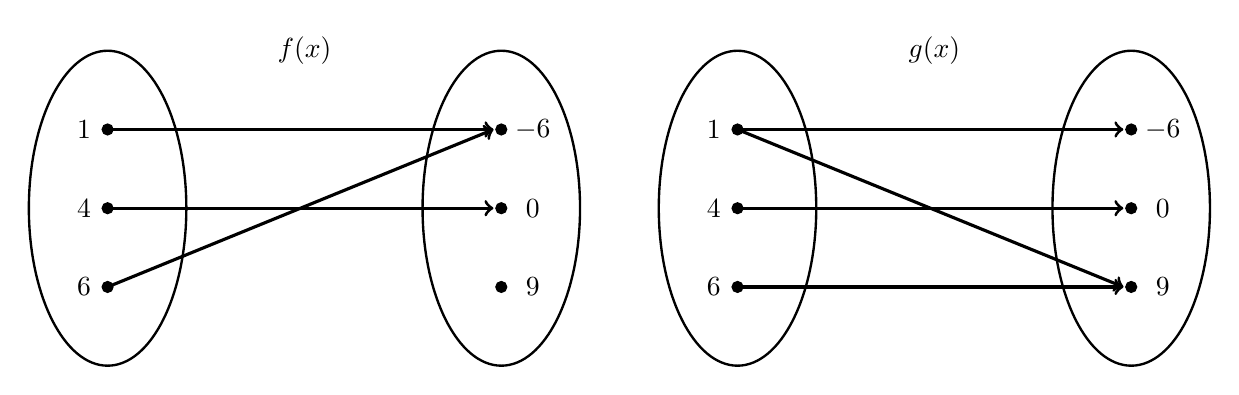
\begin{tikzpicture}
	\node at (2.5,2) {$f(x)$};
	% Ellipses
	\draw[line width=0.03cm] (0,0) circle (1 and 2);
	\draw[line width=0.03cm] (5,0) circle (1 and 2);
	
	% Nodes
	\draw[fill=black] (0,1) circle (0.07);
	\draw[fill=black] (0,0) circle (0.07);
	\draw[fill=black] (0,-1) circle (0.07);
	
	\draw[fill=black] (5,1) circle (0.07);
	\draw[fill=black] (5,0) circle (0.07);
	\draw[fill=black] (5,-1) circle (0.07);
	
	% Arrow
	\draw[line width=0.04cm,->] (0,1) -- (4.9,1);
	\draw[line width=0.04cm,->] (0,0) -- (4.9,0);
	\draw[line width=0.04cm,->] (0,-1) -- (4.9,1);
	
	% Labels
	\node at (-0.3,1) {$1$};
	\node at (-0.3,0) {$4$};
	\node at (-0.3,-1) {$6$};
	
	\node at (5.4,1) {$-6$};
	\node at (5.4,0) {$0$};
	\node at (5.4,-1) {$9$};
	
	\tikzset{shift={(8,0)}}
	%
	\node at (2.5,2) {$g(x)$};
	% Ellipses
	\draw[line width=0.03cm] (0,0) circle (1 and 2);
	\draw[line width=0.03cm] (5,0) circle (1 and 2);
	
	% Nodes
	\draw[fill=black] (0,1) circle (0.07);
	\draw[fill=black] (0,0) circle (0.07);
	\draw[fill=black] (0,-1) circle (0.07);
	
	\draw[fill=black] (5,1) circle (0.07);
	\draw[fill=black] (5,0) circle (0.07);
	\draw[fill=black] (5,-1) circle (0.07);
	
	% Arrow
	\draw[line width=0.04cm,->] (0,1) -- (4.9,1);
	\draw[line width=0.04cm,->] (0,1) -- (4.9,-1);
	\draw[line width=0.04cm,->] (0,0) -- (4.9,0);
	\draw[line width=0.04cm,->] (0,-1) -- (4.9,-1);
	
	% Labels
	\node at (-0.3,1) {$1$};
	\node at (-0.3,0) {$4$};
	\node at (-0.3,-1) {$6$};
	
	\node at (5.4,1) {$-6$};
	\node at (5.4,0) {$0$};
	\node at (5.4,-1) {$9$};
	\end{tikzpicture}
	\] \pspace


% Problem
\prob  Determine if the relations $f(x)$ and $g(x)$ shown below are functions. Explain why or why not. 
	\begin{table}[H]
	\centering
	\begin{tabular}{c|rcc|r}
	$x$ & $f(x)$ & \hspace{1cm} & $x$ & $g(x)$ \\ \cline{1-2} \cline{4-5}
	$1$ & $8$ & & $5$ & $2$ \\
	$2$ & $-7$ & & $6$ & $\pi$ \\
	$3$ & $8$ & & $8$ & $1.87$ \\
	$4$ & $8$ & & $9$ & $-9$ \\
	$5$ & $10$ & & $5$ & $3$
	\end{tabular}
	\end{table} \pspace


% Problem
\prob Determine if the relations $f(x)$ and $g(x)$ shown below are functions. Explain why or why not. 
	\[
	\begin{aligned}
	f(x)&= 2.54x + 91 \\[0.3cm]
	g(x)&= x^3 - x + 1
	\end{aligned}
	\] \pspace
   

% Problem
\prob Suppose $f(x)$ is the function given below.
	\[
	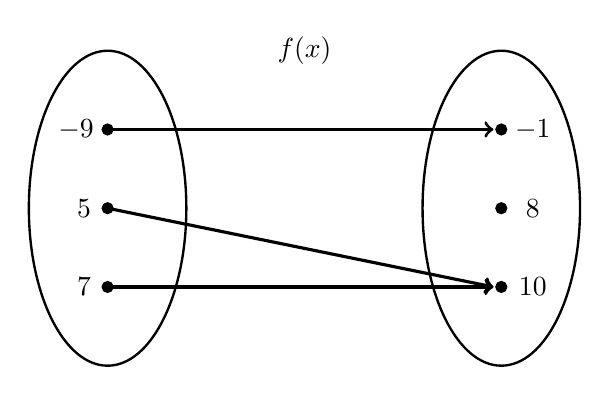
\begin{tikzpicture}
	\node at (2.5,2) {$f(x)$};
	% Ellipses
	\draw[line width=0.03cm] (0,0) circle (1 and 2);
	\draw[line width=0.03cm] (5,0) circle (1 and 2);
	
	% Nodes
	\draw[fill=black] (0,1) circle (0.07);
	\draw[fill=black] (0,0) circle (0.07);
	\draw[fill=black] (0,-1) circle (0.07);
	
	\draw[fill=black] (5,1) circle (0.07);
	\draw[fill=black] (5,0) circle (0.07);
	\draw[fill=black] (5,-1) circle (0.07);
	
	% Arrow
	\draw[line width=0.04cm,->] (0,1) -- (4.9,1);
	\draw[line width=0.04cm,->] (0,0) -- (4.9,-1);
	\draw[line width=0.04cm,->] (0,-1) -- (4.9,-1);
	
	% Labels
	\node at (-0.4,1) {$-9$};
	\node at (-0.3,0) {$5$};
	\node at (-0.3,-1) {$7$};
	
	\node at (5.4,1) {$-1$};
	\node at (5.4,0) {$8$};
	\node at (5.4,-1) {$10$};
	\end{tikzpicture}
	\]

\begin{enumerate}[(a)]
\item What is the domain of $f(x)$?
\item What is the codomain of $f(x)$?
\item What is the range of $f(x)$?
\end{enumerate} \pspace


% Problem
\prob Suppose $f(x)$ and $g(x)$ are the functions given below. 
        \begin{table}[H]
        \centering
        \begin{tabular}{| c || c | c | c | c | c | c | c |} \hline
	$x$ & $-2$ & $0$ & $1$ & $3$ & $4$ & $5$ & $10$ \\ \hline
	$f(x)$ & $5$ & $-3.1$ & $\pi$ & $5$ & $3/2$ & $14$ & $0$ \\ \hline
	$g(x)$ & $6$ & $4$ & $6.6$ & $-15$ & $4$ & $9$ & $2$ \\ \hline
        \end{tabular}
        \end{table}

Compute the following: \pspace
        \begin{enumerate}[(a)]
        \item $f(1)=$ 
        \item $g(0)=$ 
        \item $(f + g)(5)=$ 
        \item $(f - g)(-2)=$ 
        \item $(6f)(1)=$ 
        \item $\left(\dfrac{f}{g}\right)(10)=$ 
        \item $f(4)\, g(5)=$ 
        \item $f(2 - g(0))=$ 
        \item $(f \circ g)(0)=$ 
        \item $(g \circ f)(3)=$ 
        \end{enumerate} \pspace


% Problem
\prob Suppose $f(x)$ and $g(x)$ are the functions given below. 
	\[
	\begin{aligned}
	f(x)&= 3x - 1 \\[0.3cm]
	g(x)&= x^2 + x + 1
	\end{aligned}
	\]

Compute the following: 
\begin{enumerate}[(a)]
\item $f(1)=$ 
\item $g(0)=$ 
\item $f(1) - 2g(1)=$ 
\item $f(x) - g(x)=$ 
\item $f(x) \, g(x)=$ 
\item $\left( \dfrac{f}{g} \right)(x)=$ 
\item $(g \circ f)(1)=$ 
\item $f(g(0))=$ 
\item $(f \circ g)(x)=$ 
\item $(g \circ f)(x)=$ 
\end{enumerate} \pspace


% Problem
\prob Plot the function $f(x):= 4 - 3x$, being as accurate as possible. 
	\[
	\fbox{
	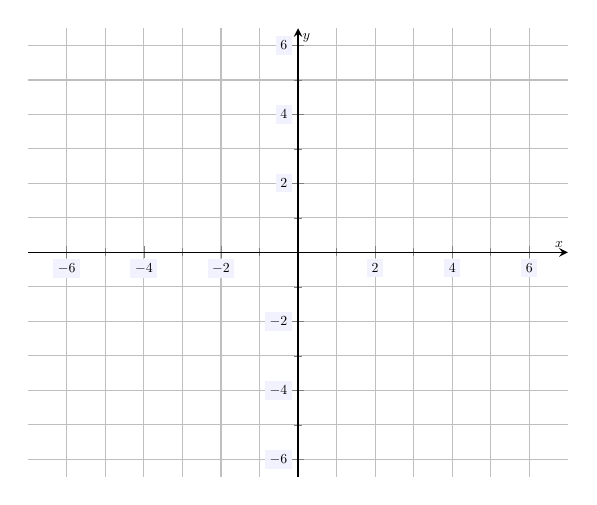
\begin{tikzpicture}[scale=1,every node/.style={scale=0.5}]
	\begin{axis}[
	grid=both,
	axis lines=middle,
	ticklabel style={fill=blue!5!white},
	xmin= -7, xmax=7,
	ymin= -6.5, ymax=6.5,
	xtick={-6,-4,-2,0,2,4,6},
	ytick={-6,-4,-2,0,2,4,6},
	minor tick = {-5,-3,...,5},
	xlabel=\(x\),ylabel=\(y\),
	]
	\end{axis}
	\end{tikzpicture}
	}
	\] \pspace


% Problem
\prob Two functions $f(x)$ and $g(x)$ are plotted below. Are $f(x)$ and $g(x)$ functions? Explain. Do the functions $f(x)$ and $g(x)$ have an inverse? Explain.  
	\[
	\fbox{
	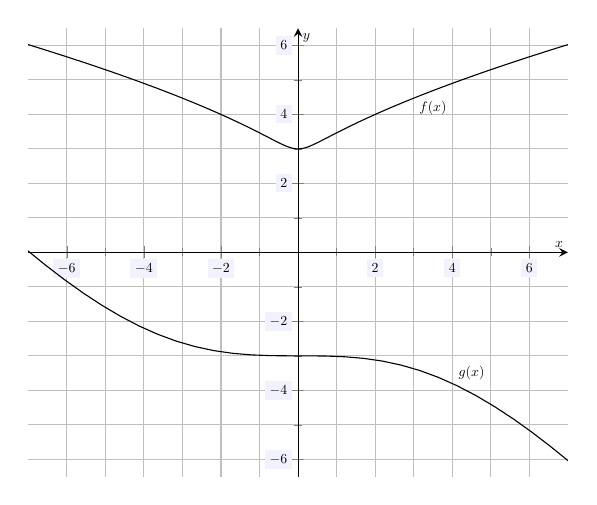
\begin{tikzpicture}[scale=1,every node/.style={scale=0.5}]
	\begin{axis}[
	grid=both,
	axis lines=middle,
	ticklabel style={fill=blue!5!white},
	xmin= -7, xmax=7,
	ymin= -6.5, ymax=6.5,
	xtick={-6,-4,-2,0,2,4,6},
	ytick={-6,-4,-2,0,2,4,6},
	minor tick = {-5,-3,...,5},
	xlabel=\(x\),ylabel=\(y\),
	]
	\node at (3.5,4.2) {$f(x)$};
	\addplot [domain= -3:3,samples=80] ({x^3 + x},{x^2 + 3}); 
	\node at (4.5,-3.5) {$g(x)$};
	\addplot [domain= -3:3,samples=100] ({8*x)},{-8*x^3/(x^2+1) - 3}); 
	\end{axis}
	\end{tikzpicture}
	}
	\] \pspace


% Problem
\prob Let $f(x)= 6x - 5$ and $g(x)= 2x^2 + 3x - 5$. 
	\begin{enumerate}[(a)]
	\item What is $g(2)$? 
	\item Assuming $g^{-1}$ exists, what is $g^{-1}(9)$?
	\item Assuming $f^{-1}$ exists, what is $f^{-1}(4)$?
	\end{enumerate} \pspace


% Problem
\prob Do the points $(1, 3)$, $(3, 7)$, and $(5,1)$ lie along a line? Justify your answer. \pspace


% Problem
\prob  Let $\ell(x)$ be the line through the points $(-2, 11)$ and $(3, -4)$.
	\begin{enumerate}[(a)]
	\item Find the slope of the line given by $\ell(x)$.
	\item Find the equation for $\ell(x)$.
	\item What is the $y$-intercept for $\ell(x)$?
	\item What is $\ell(-1)$?
	\end{enumerate} \pspace


% Problem
\prob Let $\ell(x)$ be the line through the point $(1, 3)$ with slope $\frac{1}{2}$.
	\begin{enumerate}[(a)]
	\item Find the equation for $\ell(x)$. 
	\item What is $\ell(4)$?
	\item Find the $x$-intercept for $\ell(x)$. 
	\end{enumerate} \pspace


% Problem
\prob Find the equation of the line passing through the point $(1, -1)$ that is perpendicular to the line $y= \frac{1}{3} x - 8$. \pspace


% Problem
\prob Let $f(x)= 2x - 1$. Find $f^{-1}(x)$. Show that $f^{-1}(x)$ is the inverse by showing $f(f^{-1}(x))= x$ and $f^{-1}(f(x))= x$. \pspace


% Problem
\prob A cable internet company offers a high-speed internet package that costs \$62 per month, plus an additional \$85 installation fee. 
	\begin{enumerate}[(a)]
	\item Find a function that represents the total cost of purchasing internet from this company after $n$ months. 
	\item What does the $y$-intercept for this function represent?
	\item Find the total cost of the internet after 14 months.
	\item How many months of internet can you get for \$500?
	\end{enumerate} \pspace





\newpage





% Problem
\prob Consider the following relations below:

	\[
	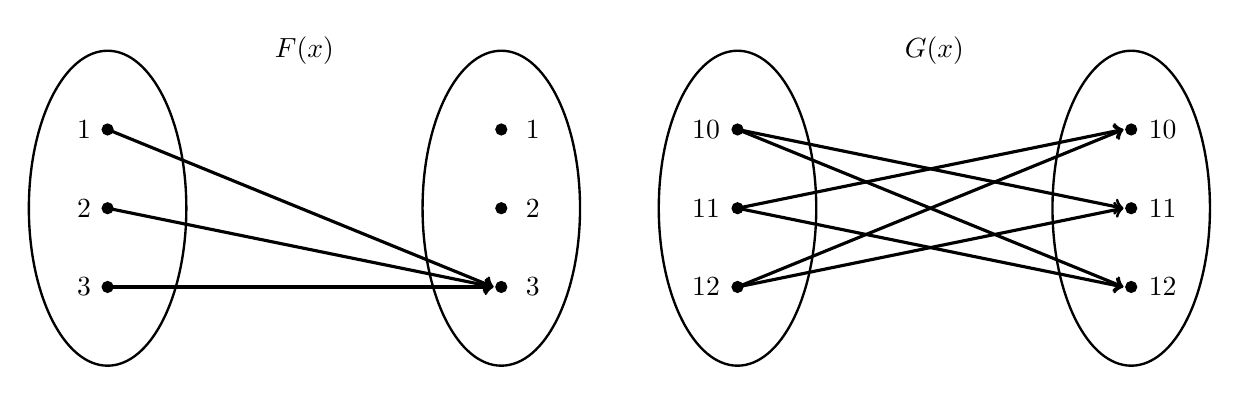
\begin{tikzpicture}
	\node at (2.5,2) {$F(x)$};
	% Ellipses
	\draw[line width=0.03cm] (0,0) circle (1 and 2);
	\draw[line width=0.03cm] (5,0) circle (1 and 2);
	
	% Nodes
	\draw[fill=black] (0,1) circle (0.07);
	\draw[fill=black] (0,0) circle (0.07);
	\draw[fill=black] (0,-1) circle (0.07);
	
	\draw[fill=black] (5,1) circle (0.07);
	\draw[fill=black] (5,0) circle (0.07);
	\draw[fill=black] (5,-1) circle (0.07);
	
	% Arrow
	\draw[line width=0.04cm,->] (0,1) -- (4.9,-1);
	\draw[line width=0.04cm,->] (0,0) -- (4.9,-1);
	\draw[line width=0.04cm,->] (0,-1) -- (4.9,-1);
	
	% Labels
	\node at (-0.3,1) {$1$};
	\node at (-0.3,0) {$2$};
	\node at (-0.3,-1) {$3$};
	
	\node at (5.4,1) {$1$};
	\node at (5.4,0) {$2$};
	\node at (5.4,-1) {$3$};
	
	\tikzset{shift={(8,0)}}
	%
	\node at (2.5,2) {$G(x)$};
	
	% Ellipses
	\draw[line width=0.03cm] (0,0) circle (1 and 2);
	\draw[line width=0.03cm] (5,0) circle (1 and 2);
	
	% Nodes
	\draw[fill=black] (0,1) circle (0.07);
	\draw[fill=black] (0,0) circle (0.07);
	\draw[fill=black] (0,-1) circle (0.07);
	
	\draw[fill=black] (5,1) circle (0.07);
	\draw[fill=black] (5,0) circle (0.07);
	\draw[fill=black] (5,-1) circle (0.07);
	
	% Arrow
	\draw[line width=0.04cm,->] (0,1) -- (4.9,0);
	\draw[line width=0.04cm,->] (0,1) -- (4.9,-1);
	\draw[line width=0.04cm,->] (0,0) -- (4.9,1);
	\draw[line width=0.04cm,->] (0,0) -- (4.9,-1);
	\draw[line width=0.04cm,->] (0,-1) -- (4.9,1);
	\draw[line width=0.04cm,->] (0,-1) -- (4.9,0);
	
	% Labels
	\node at (-0.4,1) {$10$};
	\node at (-0.4,0) {$11$};
	\node at (-0.4,-1) {$12$};
	
	\node at (5.4,1) {$10$};
	\node at (5.4,0) {$11$};
	\node at (5.4,-1) {$12$};
	\end{tikzpicture}
	\] \pspace

	\begin{minipage}[b]{0.49\textwidth}
	\centering
	\begin{tabular}{c|rcc|r}
	$x$ & $H(x)$ & \hspace{1cm} & $x$ & $J(x)$ \\ \cline{1-2} \cline{4-5}
	$1$ & $1$ & & $5$ & $-2$ \\
	$2$ & $1$ & & $6$ & $-1$ \\
	$3$ & $2$ & & $8$ & $0$ \\
	$4$ & $2$ & & $9$ & $1$ \\
	$5$ & $4$ & & $5$ & $2$
	\end{tabular}
	\end{minipage}
	\begin{minipage}[b]{0.49\textwidth}
	\[
	\begin{aligned}
	K(x)&:= 14x - 9 \\[0.6cm]
	L(x)&:= 5x(1 - x^3)
	\end{aligned}
	\]
	\end{minipage} \pvspace{0.6cm}
	
Determine if each of the relations given above is a function. \pspace


% Problem
\prob Consider the functions given in the table below.
        \begin{table}[H]
        \centering
        \begin{tabular}{| c || c | c | c | c | c |} \hline
	$x$ & $-2$ & $-1$ & $0$ & $1$ & $2$ \\ \hline
	$f(x)$ & $3$ & $-2$ & $1$ & $6$ & $0$ \\ \hline
	$g(x)$ & $1$ & $2$ & $-1$ & $-2$ & $-6$ \\ \hline
        \end{tabular}
        \end{table}

Compute the following: \pspace
        \begin{enumerate}[(a)]
        \item $f(1)=$ 
        \item $g(-1) - f(-2)=$ 
        \item $f(-1)g(0)=$ 
        \item $(f - g)(1)=$ 
        \item $(f \circ g)(-2)=$ 
        \item $(g \circ f)(2)=$ 
        \item $y$-intercept of $g(x)$: 
        \item $x$-intercept of $f(x)$: 
        \end{enumerate} \pspace


% Problem
\prob Find the equation of the line through $(-4, 12)$ and $(2, 3)$. \pspace


% Problem
\prob Find the equation of the line that is perpendicular to $y= 6$ that passes through the $x$-intercept of $y= x - 3$. \pspace


% Problem
\prob Simplify the following radical expressions: \pspace
	\begin{enumerate}[(a)]
	\item $\sqrt{36}$ 
	\item $\sqrt[3]{64}$ 
	\item $\sqrt{2^5 \cdot 3^2 \cdot 5}$ 
	\item $\sqrt[4]{2^3 \cdot 3^9 \cdot 5^4}$ 
	\end{enumerate} \pspace


% Problem
\prob Answer the following:
	\[
	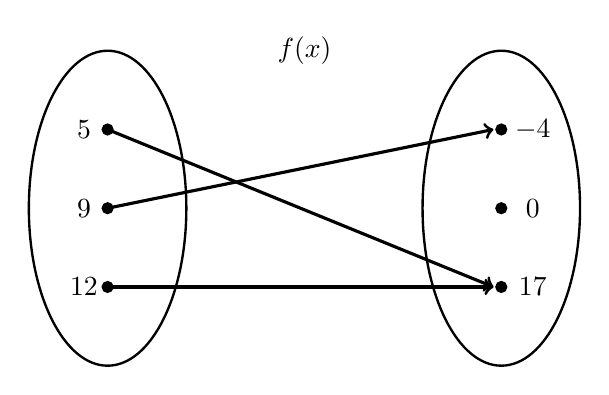
\begin{tikzpicture}
	\node at (2.5,2) {$f(x)$};
	% Ellipses
	\draw[line width=0.03cm] (0,0) circle (1 and 2);
	\draw[line width=0.03cm] (5,0) circle (1 and 2);
	
	% Nodes
	\draw[fill=black] (0,1) circle (0.07);
	\draw[fill=black] (0,0) circle (0.07);
	\draw[fill=black] (0,-1) circle (0.07);
	
	\draw[fill=black] (5,1) circle (0.07);
	\draw[fill=black] (5,0) circle (0.07);
	\draw[fill=black] (5,-1) circle (0.07);
	
	% Arrow
	\draw[line width=0.04cm,->] (0,1) -- (4.9,-1);
	\draw[line width=0.04cm,->] (0,0) -- (4.9,1);
	\draw[line width=0.04cm,->] (0,-1) -- (4.9,-1);
	
	% Labels
	\node at (-0.3,1) {$5$};
	\node at (-0.3,0) {$9$};
	\node at (-0.3,-1) {$12$};
	
	\node at (5.4,1) {$-4$};
	\node at (5.4,0) {$0$};
	\node at (5.4,-1) {$17$};
	\end{tikzpicture}
	\] \pspace

\begin{enumerate}[(a)]
\item Explain why the relation $f(x)$ above is a function. 
\item Find the domain, codomain, and range of the function $f(x)$. 
\item Is the relation $g(x)= 17x - x^3$ a function? Explain. 
\end{enumerate} \pspace


% Problem
\prob Consider the relation $f(x)$ plotted below.
	\[
	\fbox{
	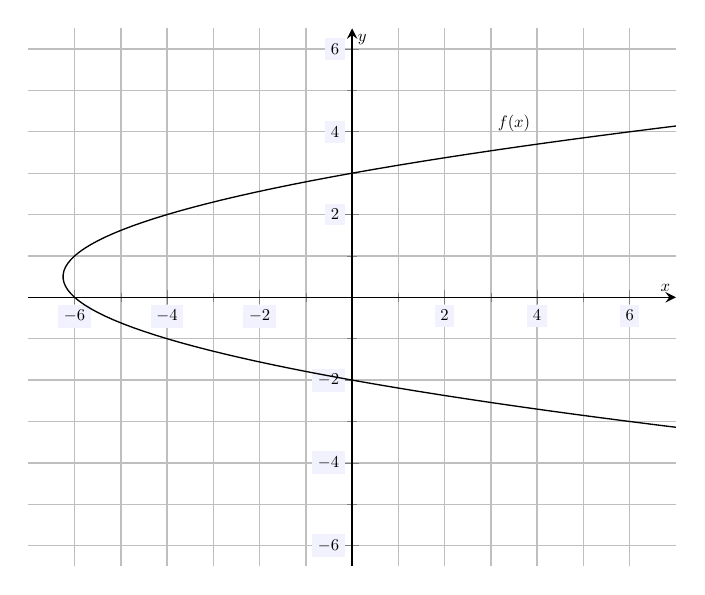
\begin{tikzpicture}[scale=1.2,every node/.style={scale=0.5}]
	\begin{axis}[
	grid=both,
	axis lines=middle,
	ticklabel style={fill=blue!5!white},
	xmin= -7, xmax=7,
	ymin= -6.5, ymax=6.5,
	xtick={-6,-4,-2,0,2,4,6},
	ytick={-6,-4,-2,0,2,4,6},
	minor tick = {-5,-3,...,5},
	xlabel=\(x\),ylabel=\(y\),
	]
	\node at (3.5,4.2) {$f(x)$};
	\addplot [domain= -4:5,samples=100] ({x^2 - x - 6},{x}); 
	\end{axis}
	\end{tikzpicture}
	}
	\] \pspace

\begin{enumerate}[(a)]
\item Is the relation $f(x)$ plotted above a function? Explain. 
\item Does the relation above have an inverse function? Explain. 
\item Find the $y$-intercepts of the relation plotted above. 
\item Find the $x$-intercepts of the relation plotted above. 
\end{enumerate} \pspace


% Problem
\prob Consider the functions given in the table below.
        \begin{table}[H]
        \centering
        \begin{tabular}{| c || r | r | r | r | r |} \hline
	$x$ & $-2$ & $-1$ & $0$ & $1$ & $2$ \\ \hline
	$f(x)$ & $5$ & $-2$ & $-5$ & $-3$ & $2$ \\ \hline
	$g(x)$ & $6$ & $2$ & $10$ & $7$ & $-5$ \\ \hline
        \end{tabular}
        \end{table}

Compute the following: \pspace
        \begin{enumerate}[(a)]
        \item $g(2)=$ 
        \item $(f - g)(0)=$ 
        \item $(fg)(1)=$ 
        \item $\left( \dfrac{g}{f} \right)(0)=$ 
        \item $(f \circ g)(-1)=$ 
        \item $(g \circ f)(-1)=$ 
        \end{enumerate} \pspace


% Problem
\prob Find the equation of the line perpendicular to $y= 6 - 2x$ at its $x$-intercept. \pspace


% Problem
\prob Solve the following equation and then verify your solution:
	\[
	3x -14= 8 - \frac{2}{3}\,x
	\] \pspace


% Problem
\prob Showing all your work, simplify the following as much as possible:
        \begin{enumerate}[(a)]
        \item $(x^{-2} y^5)^3$
        \item $\dfrac{x^{-3}y^4}{x^3y^5}$
        \item $x(x^5y)^2y^{-6}$
        \end{enumerate} \pspace


% Problem
\prob Showing all your work, simplify the following as much as possible:
        \begin{enumerate}[(a)]
        \item $\left( \dfrac{x^3}{y^{-1}} \right)^{-1}$
        \item $\dfrac{(x^2y)^0 x^4}{(y^3)^2}$
        \item $\dfrac{(x^{-3} y^4)^{-5} x^2y}{x^{-2} y^0}$
        \end{enumerate} \pspace


% Problem
\prob Showing all your work, simplify the following as much as possible:
        \begin{enumerate}[(a)]
        \item $(x^7 y^8)^{1/2}$
        \item $\left( \dfrac{\sqrt{x^5}}{\sqrt[3]{y^2}} \right)^4$
        \item $\dfrac{x(x^{3/2}y^{2/3})^2}{(x^6 y)^{1/3}}$
        \end{enumerate} \pspace


% Problem
\prob  Showing all your work, simplify the following as much as possible:
        \begin{enumerate}[(a)]
        \item $\dfrac{(y \sqrt{x})^4}{\sqrt{y}\, x^{-3/2}}$
        \item $(\sqrt[3]{y x^2})^2 (yx^2)^{1/3}$
        \item $\left( \dfrac{x^4}{y^7} \right)^{-2/3}$
        \end{enumerate} \pspace


% Problem
\prob Determine if the relations $f(x)$ and $g(x)$ shown below are functions. Explain why or why not. If the relation is a function, determine its domain, codomain, and range. 
	\[
	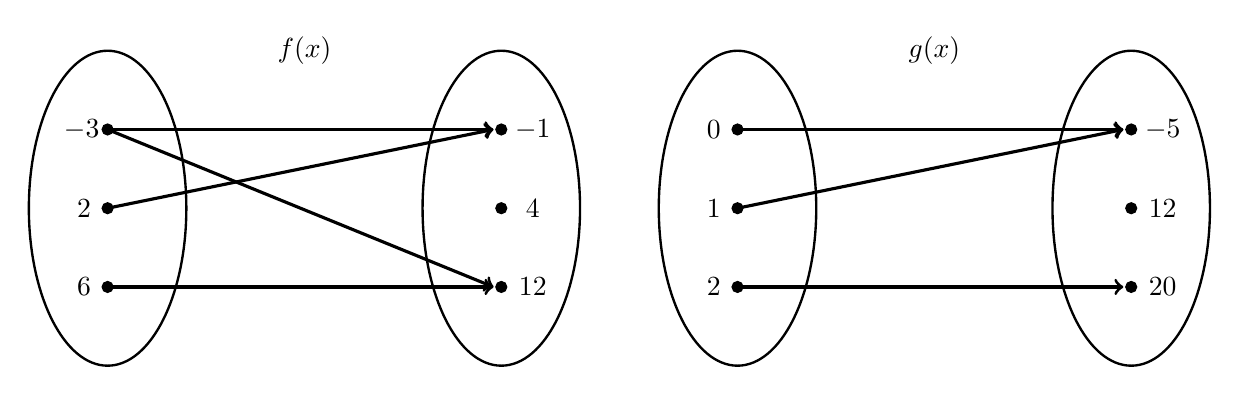
\begin{tikzpicture}
	\node at (2.5,2) {$f(x)$};
	% Ellipses
	\draw[line width=0.03cm] (0,0) circle (1 and 2);
	\draw[line width=0.03cm] (5,0) circle (1 and 2);
	
	% Nodes
	\draw[fill=black] (0,1) circle (0.07);
	\draw[fill=black] (0,0) circle (0.07);
	\draw[fill=black] (0,-1) circle (0.07);
	
	\draw[fill=black] (5,1) circle (0.07);
	\draw[fill=black] (5,0) circle (0.07);
	\draw[fill=black] (5,-1) circle (0.07);
	
	% Arrow
	\draw[line width=0.04cm,->] (0,1) -- (4.9,1);
	\draw[line width=0.04cm,->] (0,1) -- (4.9,-1);
	\draw[line width=0.04cm,->] (0,0) -- (4.9,1);
	\draw[line width=0.04cm,->] (0,-1) -- (4.9,-1);
	
	% Labels
	\node at (-0.3,1) {$\!-3$};
	\node at (-0.3,0) {$2$};
	\node at (-0.3,-1) {$6$};
	
	\node at (5.4,1) {$-1$};
	\node at (5.4,0) {$4$};
	\node at (5.4,-1) {$12$};
	
	\tikzset{shift={(8,0)}}
	%
	\node at (2.5,2) {$g(x)$};
	% Ellipses
	\draw[line width=0.03cm] (0,0) circle (1 and 2);
	\draw[line width=0.03cm] (5,0) circle (1 and 2);
	
	% Nodes
	\draw[fill=black] (0,1) circle (0.07);
	\draw[fill=black] (0,0) circle (0.07);
	\draw[fill=black] (0,-1) circle (0.07);
	
	\draw[fill=black] (5,1) circle (0.07);
	\draw[fill=black] (5,0) circle (0.07);
	\draw[fill=black] (5,-1) circle (0.07);
	
	% Arrow
	\draw[line width=0.04cm,->] (0,1) -- (4.9,1);
	\draw[line width=0.04cm,->] (0,0) -- (4.9,1);
	\draw[line width=0.04cm,->] (0,-1) -- (4.9,-1);
	
	% Labels
	\node at (-0.3,1) {$0$};
	\node at (-0.3,0) {$1$};
	\node at (-0.3,-1) {$2$};
	
	\node at (5.4,1) {$-5$};
	\node at (5.4,0) {$12$};
	\node at (5.4,-1) {$20$};
	\end{tikzpicture}
	\] \pspace


% Problem
\prob Determine if the relations $f(x)$ and $g(x)$ shown below are functions. Explain why or why not. If the relation is a function, compute the functions value at $x= 10$. 
	\[
	\begin{aligned}
	f(x)&= 47.3 - 17.9x \\[0.3cm]
	g(x)&= 2x^2 + 5x - 6
	\end{aligned}
	\] \pspace





\newpage





% Problem
\prob Suppose $f(x)$ and $g(x)$ are the functions given below. 
        \begin{table}[H]
        \centering
        \begin{tabular}{| c || c | c | c | c | c | c | c |} \hline
	$x$ & $-3$ & $-2$ & $-1$ & $\phantom{-}0$ & $\phantom{-}1$ & $\phantom{-}2$ & $\phantom{-}3$ \\ \hline
	$f(x)$ & $5$ & $2$ & $0$ & $-1$ & $-2$ & $-4$ & $-5$ \\ \hline
	$g(x)$ & $1$ & $1$ & $5$ & $2$ & $-3$ & $-3$ & $4$ \\ \hline
	$h(x)$ & $-6$ & $7$ & $1$ & $-2$ & $0$ & $1$ & $-1$ \\ \hline
        \end{tabular}
        \end{table}

Compute the following: \pspace
        \begin{enumerate}[(a)]
        \item $(f + g)(3)=$ 
        \item $(f - g)(-1)=$ 
        \item $(5h)(1)=$ 
        \item $\left(\dfrac{h}{g}\right)(-3)=$ 
        \item $f(2)\, h(-2)=$ 
        \item $h(-1 - f(0))=$ 
        \item $(g \circ f)(-2)=$ 
	\item $(h \circ g)(1)=$ 
        \item $(g \circ h)(1)=$ 
	\item $(g \circ f \circ h)(-1)=$ 
        \end{enumerate} \pspace


% Problem
\prob Suppose $f(x)$ and $g(x)$ are the functions given below. 
	\[
	\begin{aligned}
	f(x)&= 3x - 10 \\[0.3cm]
	g(x)&= 2x^2 - x + 5
	\end{aligned}
	\]

Compute the following: \pspace
\begin{enumerate}[(a)]
\item $f(3)=$ 
\item $g(-2)=$ 
\item $5f(6) - g(1)=$ 
\item $f(x) - g(x)=$ 
\item $f(x) \, g(x)=$ 
\item $\left( \dfrac{f}{g} \right)(x)=$ 
\item $(f \circ g)(0)=$ 
\item $(g \circ f)(3)=$ 
\item $(f \circ g)(x)=$ 
\item $(g \circ f)(x)=$ 
\end{enumerate} \pspace


% Problem
\prob Determine if the relation below is a function or not. If it is a function, explain why. If it is not a function, explain why. Determine also whether the relation has an inverse function. If it has an inverse function, explain why. If it does not have an inverse function, explain why not. 
	\[
	\fbox{
	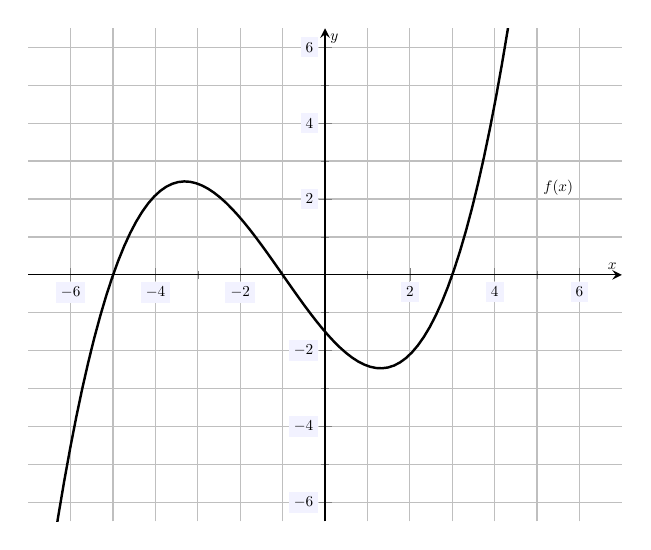
\begin{tikzpicture}[scale=1.1,every node/.style={scale=0.5}]
	\begin{axis}[
	grid=both,
	axis lines=middle,
	ticklabel style={fill=blue!5!white},
	xmin= -7, xmax=7,
	ymin= -6.5, ymax=6.5,
	xtick={-6,-4,-2,0,2,4,6},
	ytick={-6,-4,-2,0,2,4,6},
	minor tick = {-5,-3,...,5},
	xlabel=\(x\),ylabel=\(y\),
	]
	\node at (5.5,2.3) {$f(x)$};
	\addplot[thick, domain= -7:7, samples=100] ({x},{1/10*(x + 5)*(x + 1)*(x - 3)});
	\end{axis}
	\end{tikzpicture}
	}
	\] \pspace


% Problem
\prob  Determine whether the point $(2, -1)$ is on the graph of $f(x)= 2x^2 - 5x + 3$. Determine also whether the point $(1, 0)$ is on the graph of $f(x)$. For each, explain why or why not.\pspace


% Problem
\prob Consider the linear function $f(x)= 5 - \frac{3}{4}\,x$.
	\begin{enumerate}[(a)]
	\item Find the slope of this linear function. 
	\item Interpret the slope two different ways.
	\item Is the linear function increasing, decreasing, or constant? Explain. 
	\item Determine the $y$-intercept for $f(x)$.
	\item Determine the $x$-intercept for $f(x)$.
	\end{enumerate} \pspace


% Problem
\prob  Showing all your work, find the equation of the line perpendicular to $y= 5 - 3x$ that passes through the point $(1, -4)$. \pspace


% Problem
\prob Showing all your work, solve the following linear equation, be sure to verify that your solution satisfies the equation: 
	\[
	5x - 6= 1 - 7x
	\] \pspace

 
% Problem
\prob Water is flowing into a `rectangular' box with side lengths 2~ft, 4~ft, and 5~ft at a rate of 3.4~ft$^3$/min. Currently, the box contains 16~ft$^3$ of water. Let $W(t)$ denote the amount of water in the box $t$ minutes from now.
	\begin{enumerate}[(a)]
	\item Explain why $W(t)$ is linear.
	\item Find $W(t)$. 
	\item What do the slope and $y$-intercept of $W(t)$ represent in context?
	\item Determine when the box will begin to overflow. 
	\end{enumerate} \pspace


% Problem
\prob Simplify the following as much as possible, being sure to have no negative exponents in your expression: \pspace
\begin{enumerate}[(a)] 
\item $\dfrac{x^3 y^3 z}{x y^6 z^{-2}}$ 
\item $\left( \dfrac{(xy^2)^3}{x^5y} \right)^{-1}$ 
\item $\left( \dfrac{x^{-2}}{y^{-3}} \right)^{5}$ 
\item $\dfrac{15 x^{-3} y^2}{5xy}$ 
\end{enumerate} \pspace


% Problem
\prob Suppose $f(x)$ and $g(x)$ are functions whose values are given in the table below.
	\begin{table}[H]
	\centering
	\begin{tabular}{|r||c|c|c|c|c|c|} \hline
	$x$ & $-4$ & $-1$ & $\phantom{-}0$ & $\phantom{-}1$ & $\phantom{-}3$ & $\phantom{-}5$ \\ \hline
	$f(x)$ & $\phantom{-}0$ & $\phantom{-}4$ & $\phantom{-}8$ & $-1$ & $\phantom{-}7$ & $\phantom{-}4$ \\ \hline
	$g(x)$ & $-2$ & $-6$ & $-3$ & $\phantom{-}7$ & $\phantom{-}2$ & $\phantom{-}3$ \\ \hline
	\end{tabular}
	\end{table} \par
Compute the following: \pspace
        \begin{enumerate}[(a)]
        \item $g(1)$ 
        \item $(f + g)(-1)$ 
        \item $(fg)(5)$ 
        \item $(f \circ g)(5)$ 
        \item $(g \circ f)(1)$ 
        \end{enumerate} \pspace


% Problem
\prob A table of values for a function $f(x)$ is given below.
	\begin{table}[H]
	\centering
	\begin{tabular}{r||rrrrrrrrrrr}
	$x$ & $-5$ & $-4$ & $-3$ & $-2$ & $-1$ & $0$ & $1$ & $2$ & $3$ & $4$ & $5$ \\ \hline
	$f(x)$ & $6$ & $3$ & $0$ & $-2$ & $4$ & $6$ & $3$ & $0$ & $5$ & $6$ & $8$
	\end{tabular}
	\end{table} \par
Determine the $y$-intercepts and $x$-intercepts for the function $f(x)$. \pspace


% Problem
\prob A table of values for a function $f(x)$ is given below. Determine whether the function $f(x)$ is linear or not. Be sure to fully justify your answer. \par
	\begin{table}[H]
	\centering
	\begin{tabular}{r||rrrrrrrrrrr}
	$x$ & $0$ & $1$ & $2$ & $4$ & $5$ & $6$ \\ \hline
	$f(x)$ & $-5$ & $-2$ & $1$ & $7$ & $11$ & $13$
	\end{tabular}
	\end{table} \pspace


% Problem
\prob A table of values for a linear function $f(x)$ is given below.
	\begin{table}[H]
	\centering
	\begin{tabular}{r||rrrrrrrrrrr}
	$x$ & $-12$ & $-8$ & $-4$ & $\phantom{-}4$ & $\phantom{-}8$ & $\phantom{-}12$ \\ \hline
	$f(x)$ & $21$ & $18$ & $15$ & $9$ & $6$ & $3$
	\end{tabular}
	\end{table} \par
Determine the equation for $f(x)$. \pspace


% Problem
\prob Find the equation of the line that contains the points $(-10, 15)$ and $(2, -1)$. \pspace


% Problem
\prob Determine the equation of the line that contains the point $(6, 10)$ and is perpendicular to the line $y= -1$. \pspace


% Problem
\prob Find the equation of the line that is perpendicular to the line $y= 4 - 5x$ and passes through the $y$-intercept of the line $y= 2x + 3$. \pspace


% Problem
\prob A researcher creates a model to predict adolescent male's weight (in lbs) from their height (in cm). The model is $W(h)= 2.6h - 17.3$.
	\begin{enumerate}[(a)]
	\item Is the model linear? Explain.
	\item Determine the slope of $W(h)$. Interpret the slope in context.
	\item Determine the $y$-intercept of $W(h)$. Does the $y$-intercept have meaning in this context? Explain.
	\end{enumerate}  \pspace


% Problem
\prob Showing all your work, simplify the following as much as possible:
\begin{enumerate}[(a)]
\item $(x^3 y^{-1})^4$
\item $\dfrac{x^5y^{-6}}{x^3y^2}$
\item $\left( \dfrac{x^{-2}}{y^4} \right)^{-1}$
\item $\dfrac{(xy)^0 x^{-3}}{(y^2)^3}$
\item $\dfrac{(x^{-2} y^3)^{-5} xy^6}{x^0 y^{-2}}$
\end{enumerate} \pspace


% Problem
\prob Showing all your work, simplify the following as much as possible:
\begin{enumerate}[(a)]
\item $(x^4 y^5)^{1/2}$
\item $\left( \dfrac{\sqrt{x}}{\sqrt[3]{y^2}} \right)^3$
\item $\dfrac{(x \sqrt{y})^{3}}{\sqrt{x}\, y^{-3/2}}$
\item $(\sqrt[3]{x y^2})^2 (xy^2)^{1/3}$
\item $\left( \dfrac{x^6}{y^5} \right)^{-2/3}$
\end{enumerate} \pspace


% Problem
\prob Determine if the relations $f(x)$ and $g(x)$ shown below are functions. Explain why or why not. 
	\[
	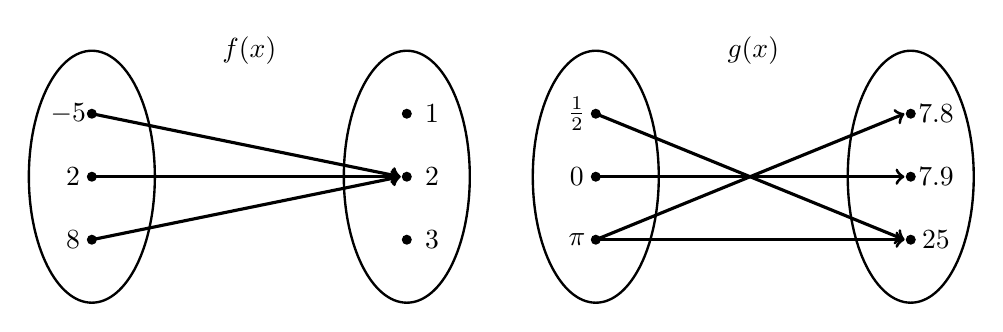
\begin{tikzpicture}[scale=0.8]
	\node at (2.5,2) {$f(x)$};
	% Ellipses
	\draw[line width=0.03cm] (0,0) circle (1 and 2);
	\draw[line width=0.03cm] (5,0) circle (1 and 2);
	
	% Nodes
	\draw[fill=black] (0,1) circle (0.07);
	\draw[fill=black] (0,0) circle (0.07);
	\draw[fill=black] (0,-1) circle (0.07);
	
	\draw[fill=black] (5,1) circle (0.07);
	\draw[fill=black] (5,0) circle (0.07);
	\draw[fill=black] (5,-1) circle (0.07);
	
	% Arrow
	\draw[line width=0.04cm,->] (0,1) -- (4.9,0);
	\draw[line width=0.04cm,->] (0,0) -- (4.9,0);
	\draw[line width=0.04cm,->] (0,-1) -- (4.9,0);
	
	% Labels
	\node at (-0.3,1) {$\!\!-5$};
	\node at (-0.3,0) {$2$};
	\node at (-0.3,-1) {$8$};
	
	\node at (5.4,1) {$1$};
	\node at (5.4,0) {$2$};
	\node at (5.4,-1) {$3$};
	
	\tikzset{shift={(8,0)}}
	%
	\node at (2.5,2) {$g(x)$};
	% Ellipses
	\draw[line width=0.03cm] (0,0) circle (1 and 2);
	\draw[line width=0.03cm] (5,0) circle (1 and 2);
	
	% Nodes
	\draw[fill=black] (0,1) circle (0.07);
	\draw[fill=black] (0,0) circle (0.07);
	\draw[fill=black] (0,-1) circle (0.07);
	
	\draw[fill=black] (5,1) circle (0.07);
	\draw[fill=black] (5,0) circle (0.07);
	\draw[fill=black] (5,-1) circle (0.07);
	
	% Arrow
	\draw[line width=0.04cm,->] (0,1) -- (4.9,-1);
	\draw[line width=0.04cm,->] (0,0) -- (4.9,0);
	\draw[line width=0.04cm,->] (0,-1) -- (4.9,1);
	\draw[line width=0.04cm,->] (0,-1) -- (4.9,-1);
	
	% Labels
	\node at (-0.3,1) {$\frac{1}{2}$};
	\node at (-0.3,0) {$0$};
	\node at (-0.3,-1) {$\pi$};
	
	\node at (5.4,1) {$7.8$};
	\node at (5.4,0) {$7.9$};
	\node at (5.4,-1) {$25$};
	\end{tikzpicture}
	\] \pspace


% Problem
\prob Determine if the relations $f(x)$ and $g(x)$ shown below are functions. Explain why or why not. 
	\begin{table}[H]
	\centering
	\begin{tabular}{c|rcc|r}
	$x$ & $f(x)$ & \hspace{1cm} & $x$ & $g(x)$ \\ \cline{1-2} \cline{4-5}
	$1$ & $5$ & & $1$ & $6$ \\
	$2$ & $5$ & & $2$ & $8$ \\
	$3$ & $6$ & & $3$ & $10$ \\
	$4$ & $6$ & & $4$ & $12$ \\
	$5$ & $10$ & & $1$ & $13$
	\end{tabular}
	\end{table} \pspace


% Problem
\prob Determine if the relation below is a function or not. If it is a function, explain why. If it is not a function, explain why. 
	\[
	\fbox{
	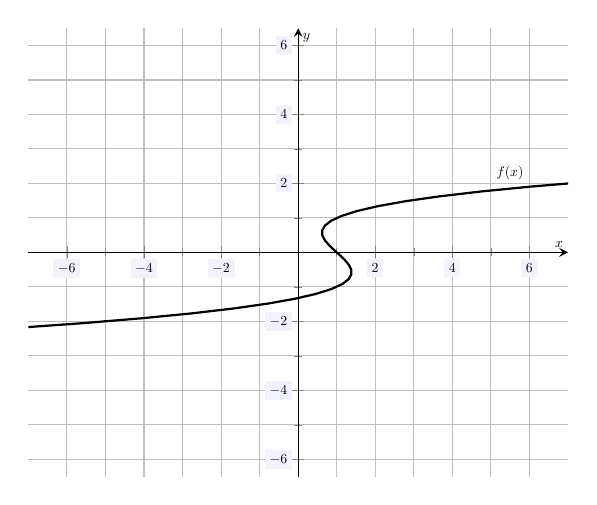
\begin{tikzpicture}[scale=1,every node/.style={scale=0.5}]
	\begin{axis}[
	grid=both,
	axis lines=middle,
	ticklabel style={fill=blue!5!white},
	xmin= -7, xmax=7,
	ymin= -6.5, ymax=6.5,
	xtick={-6,-4,-2,0,2,4,6},
	ytick={-6,-4,-2,0,2,4,6},
	minor tick = {-5,-3,...,5},
	xlabel=\(x\),ylabel=\(y\),
	]
	\node at (5.5,2.3) {$f(x)$};
	\addplot[thick, domain= -7:7, samples=100] ({x^3-x+1},{x});
	\end{axis}
	\end{tikzpicture}
	}
	\] \pspace


% Problem
\prob Determine if the relations $f(x)$ and $g(x)$ shown below are functions. Explain why or why not. 
	\[
	\begin{aligned}
	f(x)&= 6.73 - 13.54x \\[0.3cm]
	g(x)&= \dfrac{6x - 5}{3x^2 + 1}
	\end{aligned}
	\] \pspace


% Problem
\prob Suppose $f(x)$ is the function given below.
	\[
	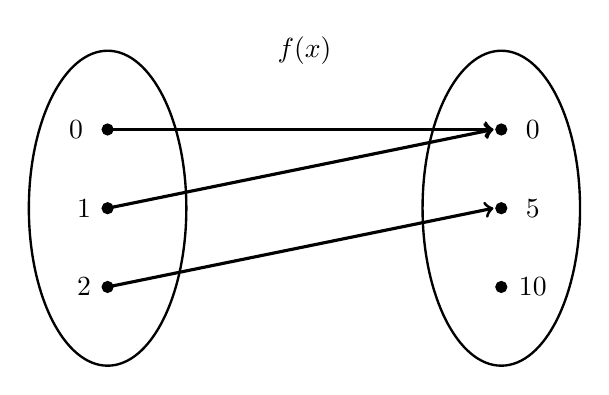
\begin{tikzpicture}
	\node at (2.5,2) {$f(x)$};
	% Ellipses
	\draw[line width=0.03cm] (0,0) circle (1 and 2);
	\draw[line width=0.03cm] (5,0) circle (1 and 2);
	
	% Nodes
	\draw[fill=black] (0,1) circle (0.07);
	\draw[fill=black] (0,0) circle (0.07);
	\draw[fill=black] (0,-1) circle (0.07);
	
	\draw[fill=black] (5,1) circle (0.07);
	\draw[fill=black] (5,0) circle (0.07);
	\draw[fill=black] (5,-1) circle (0.07);
	
	% Arrow
	\draw[line width=0.04cm,->] (0,1) -- (4.9,1);
	\draw[line width=0.04cm,->] (0,0) -- (4.9,1);
	\draw[line width=0.04cm,->] (0,-1) -- (4.9,0);
	
	% Labels
	\node at (-0.4,1) {$0$};
	\node at (-0.3,0) {$1$};
	\node at (-0.3,-1) {$2$};
	
	\node at (5.4,1) {$0$};
	\node at (5.4,0) {$5$};
	\node at (5.4,-1) {$10$};
	\end{tikzpicture}
	\]

\begin{enumerate}[(a)]
\item What is the domain of $f(x)$?
\item What is the codomain of $f(x)$?
\item What is the range of $f(x)$?
\end{enumerate} \pspace


% Problem
\prob Suppose $f(x)$ and $g(x)$ are the functions given below. 
        \begin{table}[H]
        \centering
        \begin{tabular}{| c || c | c | c | c | c | c | c |} \hline
	$x$ & $-3$ & $-2$ & $-1$ & $\phantom{-}0$ & $\phantom{-}1$ & $\phantom{-}2$ & $\phantom{-}3$ \\ \hline
	$f(x)$ & $3$ & $-2$ & $1$ & $6$ & $4$ & $-7$ & $0$ \\ \hline
	$g(x)$ & $2$ & $1$ & $0$ & $3$ & $-5$ & $-5$ & $-4$ \\ \hline
	$h(x)$ & $0$ & $1$ & $0$ & $3$ & $0$ & $-1$ & $6$ \\ \hline
        \end{tabular}
        \end{table}

Compute the following: \pspace
        \begin{enumerate}[(a)]
        \item $(f + g)(1)=$ 
        \item $(f - g)(-2)=$ 
        \item $(-2h)(3)=$ 
        \item $\left(\dfrac{h}{g}\right)(0)=$ 
        \item $f(0)\, h(-2)=$ 
        \item $f(2 - h(0))=$ 
        \item $(f \circ g)(0)=$ 
        \item $(g \circ h)(2)=$ 
        \item $(f \circ g \circ h)(1)=$ 
        \item $(h \circ g)(-2)=$
        \end{enumerate} \pspace


% Problem
\prob Suppose $f(x)$ and $g(x)$ are the functions given below. 
	\[
	\begin{aligned}
	f(x)&= 4 - 3x \\[0.3cm]
	g(x)&= x^2 - x + 4
	\end{aligned}
	\]

Compute the following: \pspace
\begin{enumerate}[(a)]
\item $f(2)=$ 
\item $g(1)=$ 
\item $3f(1) - g(2)=$ 
\item $f(x) - g(x)=$ 
\item $f(x) \, g(x)=$ 
\item $\left( \dfrac{f}{g} \right)(x)=$ 
\item $(f \circ g)(0)=$ 
\item $(g \circ f)(1)=$ 
\item $(f \circ g)(x)=$ 
\item $(g \circ f)(x)=$ 
\end{enumerate} \pspace


% Problem
\prob Given the graph of $f(x)$, sketch the function $f^{-1}(x)$. Determine also $f^{-1}(1)$ and $f^{-1}(2)$. 
	\[
	\fbox{
	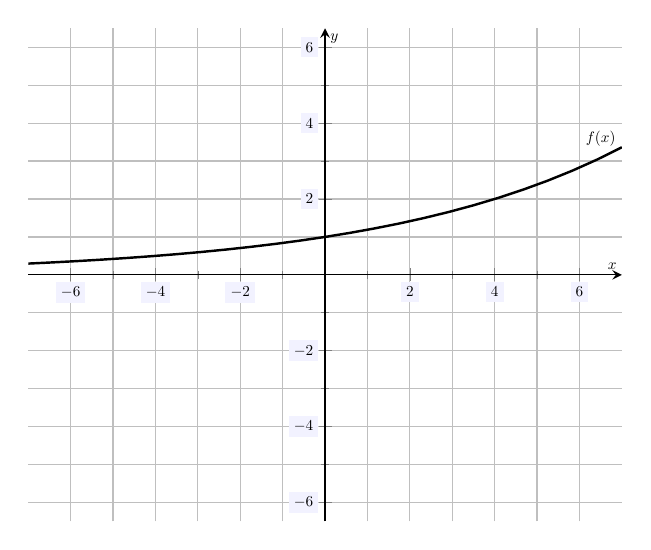
\begin{tikzpicture}[scale=1.1,every node/.style={scale=0.5}]
	\begin{axis}[
	grid=both,
	axis lines=middle,
	ticklabel style={fill=blue!5!white},
	xmin= -7, xmax=7,
	ymin= -6.5, ymax=6.5,
	xtick={-6,-4,-2,0,2,4,6},
	ytick={-6,-4,-2,0,2,4,6},
	minor tick = {-5,-3,...,5},
	xlabel=\(x\),ylabel=\(y\),
	]
	\node at (6.5,3.6) {$f(x)$};
	\addplot[thick, domain= -7:7] {2^(x/4)};
	\end{axis}
	\end{tikzpicture}
	}
	\] \pspace





\newpage





% Problem
\prob Determine if the following function is linear. Explain why or why not.
	\begin{table}[H]
	\centering
	\begin{tabular}{c|c}
	$x$ & $f(x)$ \\ \hline
	$1.2$ & $7.16$ \\
	$2.8$ & $12.39$ \\
	$4.4$ & $16.12$ \\
	$6.0$ & $22.13$ \\
	$7.6$ & $25.08$
	\end{tabular}
	\end{table} \pspace


% Problem
\prob A linear function has a table whose values are given below. Find the equation of the linear function. Be sure to specify the slope and $y$-intercept.
	\begin{table}[H]
	\centering
	\begin{tabular}{c|c}
	$x$ & $f(x)$ \\ \hline
	$2$ & $20$ \\
	$7$ & $-5$ \\
	$12$ & $-30$ \\
	$17$ & $-55$
	\end{tabular}
	\end{table} \pspace


% Problem
\prob Suppose water is draining from a tank. The number of gallons of water in the tank $t$ hours from now is given by $W(t)= 567.8 - 24.1t$.
\begin{enumerate}[(a)]
\item Is $W(t)$ linear? Explain.
\item What is the slope of $W(t)$? Interpret the slope.
\item Explain how we can know that water is draining from the tank using (b).
\item What is the $y$-intercept for $W(t)$? Interpret this intercept. 
\item Sketch a plot of $W(t)$ and estimate when the tank will be completely empty. 
\end{enumerate} \pspace


% Problem
\prob Consider the linear equation $12x - 2y= 56$. 
\begin{enumerate}[(a)]
\item Solve the linear equation for $y$. 
\item Determine the slope and $y$-intercept for the corresponding line.
\item Interpret the slope in at least two different ways. 
\end{enumerate} \pspace


% Problem
\prob Consider the linear equation $7.6x + 14.9y= 429.1$. 
\begin{enumerate}[(a)]
\item Solve the linear equation for $y$. 
\item Determine the slope and $y$-intercept for the corresponding line.
\item Interpret the slope in at least two different ways. 
\end{enumerate} \pspace





\newpage





% Problem
\prob Consider the line given by $y= -\frac{7}{6}x + 5$.
\begin{enumerate}[(a)]
\item Put the line in standard form.
\item Is the point $(-6, 10)$ on the line? Explain.
\item Is the point $(12, -9)$ on the line? Explain. 
\end{enumerate} \pspace


% Problem
\prob Find the equation of the line with slope $-\frac{15}{4}$ and $y$-intercept $(0, -8)$. \pspace


% Problem
\prob Find the equation of the line with slope $5$ passing through the point $(-3, 10)$. \pspace


% Problem
\prob A linear function is plotted below. Find the equation of this linear function. 
	\[
	\fbox{
	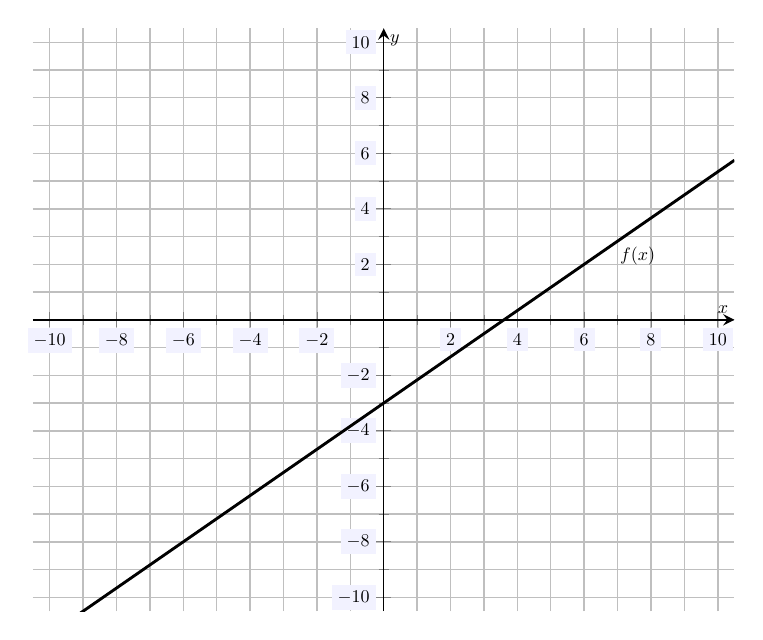
\begin{tikzpicture}[scale=1.3,every node/.style={scale=0.5}]
	\begin{axis}[
	grid=both,
	axis lines=middle,
	ticklabel style={fill=blue!5!white},
	xmin= -10.5, xmax=10.5,
	ymin= -10.5, ymax=10.5,
	xtick={-10,-8,-6,-4,-2,0,2,4,6,8,10},
	ytick={-10,-8,-6,-4,-2,0,2,4,6,8,10},
	minor tick = {-10,-9,...,10},
	xlabel=\(x\),ylabel=\(y\),
	]
	\node at (7.6,2.3) {$f(x)$};
	\addplot[thick, domain= -10.5:10.5] ({x},{5/6*x - 3});
	\end{axis}
	\end{tikzpicture}
	}
	\] \pspace


% Problem
\prob Find the equation of the line passing through the points $(6, 21)$ and $(-9, -19)$. \pspace


% Problem
\prob Find the equation of the line perpendicular to $y= 4 - 5x$ that passes through the point $(3, -1)$. \pspace


% Problem
\prob Find the equation of the line parallel to the line $x= -5$ containing the point $(4, 19)$. \pspace


% Problem
\prob Sunita works at an advertising firm. Upon hire, she was paid a \$5,000 signing bonus. The company pays her a yearly salary of \$63,000. 
        \begin{enumerate}[(a)]
        \item Write a function which gives the amount of money Sunita has been paid by the company in $t$ years. 
        \item What is the slope and $y$-intercept for the function in (a)? Interpret both of these in the problem context. 
        \item Find the amount of money Sunita has been paid in 5~years.
        \item How many years until Sunita has been paid a total of \$200,000. 
        \end{enumerate} \pspace


% Problem
\prob A tour bus company charged a group of 30~people a total of \$180 for a tour. The following week, they charged a group of 50~people \$220.
        \begin{enumerate}[(a)]
        \item Find a linear function, $C(p)$, for the total cost for a tour for a group of size $p$. 
        \item What is the slope of $C(p)$? Interpret the slope in context. 
        \item What is the $y$-intercept? Does it have meaning in this context? Explain. 
        \item Estimate much would the company charge for a group of 60~people.
        \item If you only had \$570, what would you estimate the largest group you could take on the tour?
        \end{enumerate} \pspace


% Problem
\prob A used car was purchased for \$7,500. Each year, the car loses \$1,200 in value.
        \begin{enumerate}[(a)]
        \item Find a function, $V(t)$, which gives the value, $V$, for the car after $t$ years.
        \item What does the slope of $V(t)$ represent?
        \item What does the $y$-intercept of $V(t)$ represent?
        \item What is the car worth in 3~years?
        \item How long until the car is essentially worthless? 
        \end{enumerate} \pspace


% Problem
\prob Simplify the follow expressions, showing all your work and using no negative powers:
	\begin{enumerate}[(a)] \itemsep=0.3cm
	\item $x^5 y^2 (xy^3)^0 (x^3y)^4$
	\item $z^4(x^5 z^3)^{-2} (x^3 y^2)^2$
	\item $\dfrac{x^{-5} y^6}{(x^3 y^{-4})^{-2}}$
	\item $\dfrac{(x^8 y^{12})^{1/4}}{\sqrt{x^4 y^5}}$
	\end{enumerate} \pspace


% Problem
\prob Determine whether the relations $f(x)$ and $g(x)$ shown below are functions. If the relation is a function, explain why. If the relation is not a function, explain why not. 
	\[
	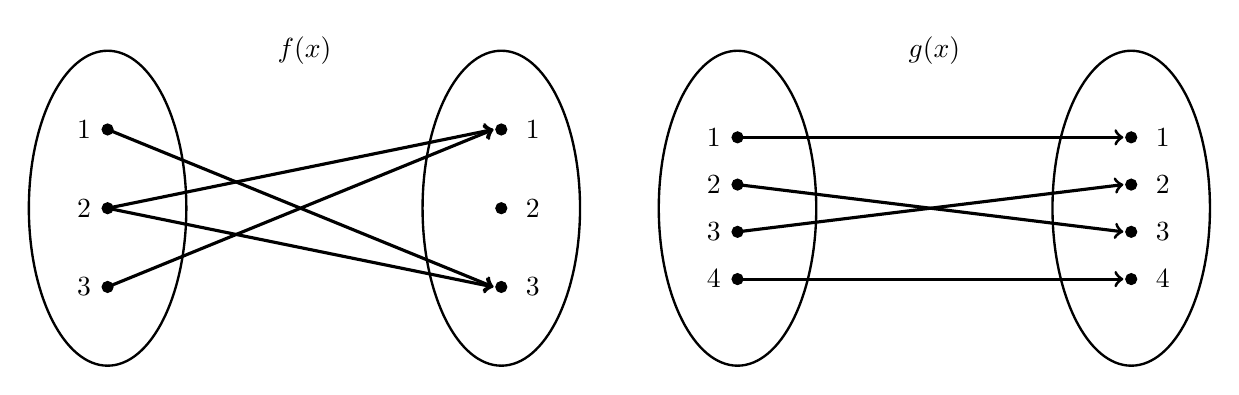
\begin{tikzpicture}
	\node at (2.5,2) {$f(x)$};
	% Ellipses
	\draw[line width=0.03cm] (0,0) circle (1 and 2);
	\draw[line width=0.03cm] (5,0) circle (1 and 2);
	
	% Nodes
	\draw[fill=black] (0,1) circle (0.07);
	\draw[fill=black] (0,0) circle (0.07);
	\draw[fill=black] (0,-1) circle (0.07);
	
	\draw[fill=black] (5,1) circle (0.07);
	\draw[fill=black] (5,0) circle (0.07);
	\draw[fill=black] (5,-1) circle (0.07);
	
	% Arrow
	\draw[line width=0.04cm,->] (0,1) -- (4.9,-1);
	\draw[line width=0.04cm,->] (0,0) -- (4.9,1);
	\draw[line width=0.04cm,->] (0,0) -- (4.9,-1);
	\draw[line width=0.04cm,->] (0,-1) -- (4.9,1);
	
	% Labels
	\node at (-0.3,1) {$1$};
	\node at (-0.3,0) {$2$};
	\node at (-0.3,-1) {$3$};
	
	\node at (5.4,1) {$1$};
	\node at (5.4,0) {$2$};
	\node at (5.4,-1) {$3$};
	
	\tikzset{shift={(8,0)}}
	%
	\node at (2.5,2) {$g(x)$};
	% Ellipses
	\draw[line width=0.03cm] (0,0) circle (1 and 2);
	\draw[line width=0.03cm] (5,0) circle (1 and 2);
	
	% Nodes
	\draw[fill=black] (0,0.9) circle (0.07);
	\draw[fill=black] (0,0.3) circle (0.07);
	\draw[fill=black] (0,-0.3) circle (0.07);
	\draw[fill=black] (0,-0.9) circle (0.07);
	
	\draw[fill=black] (5,0.9) circle (0.07);
	\draw[fill=black] (5,0.3) circle (0.07);
	\draw[fill=black] (5,-0.3) circle (0.07);
	\draw[fill=black] (5,-0.9) circle (0.07);
	
	% Arrow
	\draw[line width=0.04cm,->] (0,0.9) -- (4.9,0.9);
	\draw[line width=0.04cm,->] (0,0.3) -- (4.9,-0.3);
	\draw[line width=0.04cm,->] (0,-0.3) -- (4.9,0.3);
	\draw[line width=0.04cm,->] (0,-0.9) -- (4.9,-0.9);

	
	% Labels
	\node at (-0.3,0.9) {$1$};
	\node at (-0.3,0.3) {$2$};
	\node at (-0.3,-0.3) {$3$};
	\node at (-0.3,-0.9) {$4$};
	
	\node at (5.4,0.9) {$1$};
	\node at (5.4,0.3) {$2$};
	\node at (5.4,-0.3) {$3$};
	\node at (5.4,-0.9) {$4$};
	\end{tikzpicture}
	\] \pspace





\newpage





% Problem
\prob Consider the linear function $f(x)= \dfrac{4 - 3x}{2}$.
	\begin{enumerate}[(a)]
	\item Find the slope of this linear function. 
	\item Interpret the slope two different ways.
	\item Is the linear function increasing, decreasing, or constant? Explain. 
	\item Determine the $y$-intercept for $f(x)$.
	\item Determine the $x$-intercept for $f(x)$.
	\end{enumerate} \pspace


% Problem
\prob Determine whether the relation shown below is a function. If the relation is a function, explain why. If the relation is not a function, explain why not. 
	\[
	\fbox{
	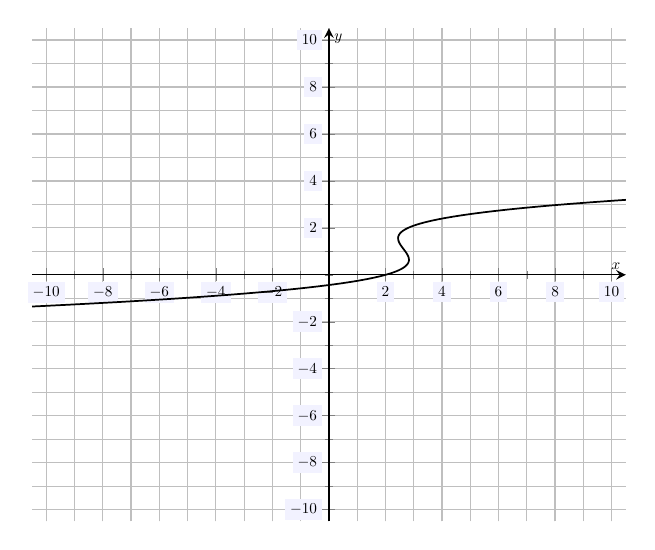
\begin{tikzpicture}[scale=1.1,every node/.style={scale=0.5}]
	\begin{axis}[
	grid=both,
	axis lines=middle,
	ticklabel style={fill=blue!5!white},
	xmin= -10.5, xmax=10.5,
	ymin= -10.5, ymax=10.5,
	xtick={-10,-8,-6,-4,-2,0,2,4,6,8,10},
	ytick={-10,-8,-6,-4,-2,0,2,4,6,8,10},
	minor tick = {-10,-9,...,10},
	xlabel=\(x\),ylabel=\(y\),
	]
	\addplot[line width= 0.02cm,domain= -2:4, samples=100] ({x^3 - 3.3*x^2 + 3*x + 2},{x}); 
	\end{axis}
	\end{tikzpicture}
	}
	\] \pspace


% Problem
\prob For the relation shown below, determine the $x$ and $y$-intercepts. 
	\[
	\fbox{
	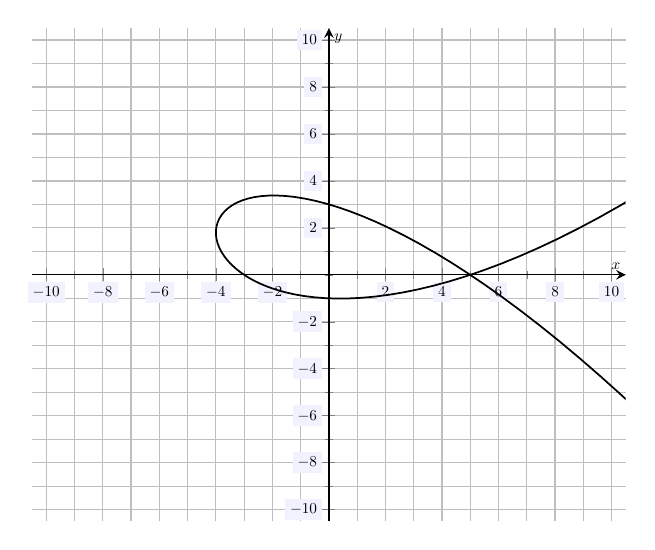
\begin{tikzpicture}[scale=1.1,every node/.style={scale=0.5}]
	\begin{axis}[
	grid=both,
	axis lines=middle,
	ticklabel style={fill=blue!5!white},
	xmin= -10.5, xmax=10.5,
	ymin= -10.5, ymax=10.5,
	xtick={-10,-8,-6,-4,-2,0,2,4,6,8,10},
	ytick={-10,-8,-6,-4,-2,0,2,4,6,8,10},
	minor tick = {-10,-9,...,10},
	xlabel=\(x\),ylabel=\(y\),
	]
	\addplot[line width= 0.02cm,domain= -10:10, samples=100] ({1/4*(x - 3)*(x + 5)},{1/40*(x - 5)*(x - 1)*(x + 7)}); 
	\end{axis}
	\end{tikzpicture}
	}
	\] \pspace





\newpage





% Problem
\prob Suppose $f(x)$, $g(x)$, and $h(x)$ are functions whose values are given below.
        \begin{table}[H]
        \centering
        \begin{tabular}{| c || r | r | r | r | r | r | r |} \hline
	$x$ & $-5$ & $-3$ & $-1$ & $\phantom{-}0$ & $\phantom{-}2$ & $\phantom{-}6$ & $\phantom{-}10$ \\ \hline \hline
	$f(x)$ & $7$ & $10$ & $0$ & $\tfrac{2}{3}$ & $-4$ & $2$ & $\sqrt{2}$ \\ \hline
	$g(x)$ & $0$ & $\pi$ & $6$ & $\tfrac{4}{5}$ & $1$ & $-3$ & $4$ \\ \hline
	$h(x)$ & $\tfrac{9}{8}$ & $0$ & $-3$ & $-1$ & $-1$ & $8$ & $-8$ \\ \hline
        \end{tabular}
        \end{table}

Compute the following, simplifying as much as possible: \pspace
        \begin{enumerate}[(a)]
        \item $(f + h)(-1)=$ 
        \item $(h - f)(10)=$ 
        \item $(-2g)(2)=$ 
        \item $\left( \dfrac{h}{f} \right)(0)=$ 
        \item $g(-3)\, h(6)=$ 
        \item $h(2 - f(2))=$ 
        \item $(g \circ h)(0)=$ 
	\item $(f \circ g)(-5)=$ 
        \item $(g \circ f)(6)=$ 
	\item $(g \circ f \circ h)(-1)=$ 
        \end{enumerate} \pspace


% Problem
\prob Suppose $f(x)$ and $g(x)$ are the functions given below. 
	\[
	\begin{aligned}
	f(x)&= 1 - x^2 \\[0.3cm]
	g(x)&= 2x + 1
	\end{aligned}
	\]

Compute the following, simplifying as much as possible: \pspace
        \begin{enumerate}[(a)]
	\item $\left( \dfrac{f}{g} \right)(x)=$ 
        \item $g(x) - f(x)=$ 
        \item $f(x) \, g(x)=$ 
        \item $(f \circ g)(x)=$ 
        \item $(g \circ f)(x)=$ 
        \end{enumerate} \pspace


% Problem
\prob Suppose that $f(x)$ is a function defined on all real numbers whose inverse exists. A few values of $f(x)$ are given below.
        \begin{table}[H]
        \centering
        \begin{tabular}{c || r | r | r | r} 
	$x$ & $1$ & $2$ & $3$ & $4$ \\ \hline
	$f(x)$ & $3$ & $4$ & $1$ & $2$
        \end{tabular}
        \end{table}

Compute the following: \pspace
	\begin{enumerate}[(a)]
	\item $f(4)=$ 
	\item $\big( f(1) \big)^2=$ 
	\item $f^{-1}(3)=$ 
	\item $f^{-1}(f(20))=$ 
	\item $(f \circ f^{-1})(5)=$ 
	\end{enumerate} \pspace


% Problem
\prob Explain whether the relation shown below has an inverse. If it does, sketch the inverse. If it does not, explain why. 
	\[
	\fbox{
	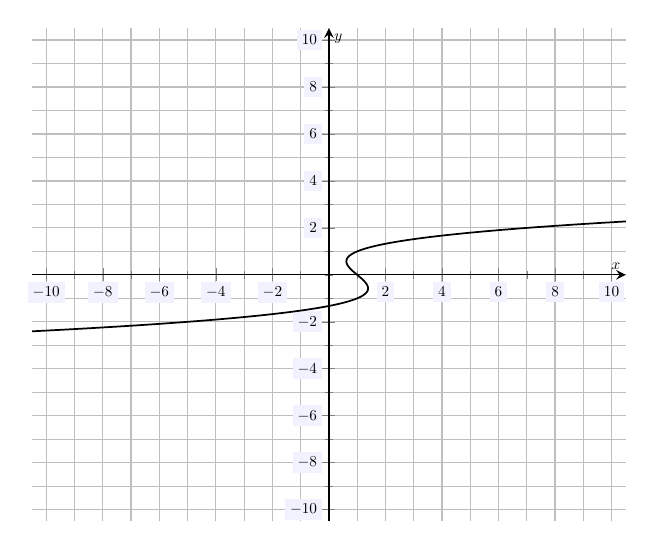
\begin{tikzpicture}[scale=1.1,every node/.style={scale=0.5}]
	\begin{axis}[
	grid=both,
	axis lines=middle,
	ticklabel style={fill=blue!5!white},
	xmin= -10.5, xmax=10.5,
	ymin= -10.5, ymax=10.5,
	xtick={-10,-8,-6,-4,-2,0,2,4,6,8,10},
	ytick={-10,-8,-6,-4,-2,0,2,4,6,8,10},
	minor tick = {-10,-9,...,10},
	xlabel=\(x\),ylabel=\(y\),
	]
	\addplot[line width= 0.02cm,domain= -3:3, samples=100] ({x^3 - x +1},{x});
	\end{axis}
	\end{tikzpicture}
	}
	\] \pspace


% Problem
\prob Determine whether the table of values below could be given by a linear function. If not, explain why. If it can, find the linear function.
        \begin{table}[H]
        \centering
        \begin{tabular}{|c || r | r | r |} \hline
	$x$ & $0.2$ & $3.6$ & $5.1$ \\ \hline
	$y$ & $9.84$ & $-1.38$ & $-6.33$ \\ \hline
        \end{tabular}
        \end{table} \pspace


% Problem
\prob Consider the line $4x - 6y= 12$.
	\begin{enumerate}[(a)]
	\item Determine the slope of the given line.
	\item Interpret the slope in at least two different ways.
	\item Is the function whose graph is the given line an increasing or decreasing function? Explain. 
	\item Determine the $y$-intercept of the given line. 
	\item Determine the $x$-intercept of the given line. 
	\end{enumerate} \pspace


% Problem
\prob A caterer charges a flat fee for each person for whom a meal has to be prepared. The caterer charges \$270 for 15 people and \$360 for 20 people. Let $C(p)$ denote the cost of hiring the caterer to prepare food for $p$ people. 
	\begin{enumerate}[(a)]
	\item Explain why $C(p)$ is linear.
	\item Find $C(p)$.
	\item Interpret the slope of $C(p)$ in the context of the problem. 
	\item Find and interpret $C(32)$. 
	\end{enumerate} \pspace


% Problem
\prob A certain species of fungus reproduces by releasing tiny spores. The larger the fungus, the more spores that are released. Scientists find that the number of spores (in thousands) a fungus with diameter $d$ (in inches) can be modeled by $N(d)= -3.5 + 15.5d$.
	\begin{enumerate}[(a)]
	\item Find and interpret the slope of $N(d)$ in the context of the problem.
	\item Find and interpret in the context of the problem, if possible, the $y$-intercept of $N(d)$.
	\item According to the model, how large would the fungus have to be in order for it to release 100,000 spores?
	\end{enumerate} \pspace


% Problem
\prob Showing all your work, find the equation of the line whose $x$-intercept is $(-1, 0)$ that has slope $-\frac{6}{7}$. \pspace


% Problem
\prob Showing all your work, find the equation of the line that is parallel to the line $x= 4$ that contains the $y$-intercept of the line $-6x + 5y= 11$. \pspace


% Problem
\prob Showing all your work, find the equation of the line that is perpendicular to the line $y= 6 - 7x$ at its $y$-intercept. \pspace


% Problem
\prob Showing all your work, solve the following equation and then verify your solution:
	\[
	6 \left( \dfrac{1}{2}\,x + 5 \right)= 28
	\] \pspace


% Problem
\prob Showing all your work, solve the following equation:
	\[
	7x + 4= 6 - 2(3 - x)
	\] \pspace


% Problem
\prob Showing all your work, solve the following equation:
	\[
	\sqrt{2} \left( x - \sqrt{2} \right)= \dfrac{x + 5}{3}
	\] \pspace


% Problem
\prob Showing all your work, solve the following equation:
	\[
	\dfrac{x + 6}{1 - x}= 10
	\] \pspace


% Problem
\prob Using no negative powers, being sure each variable appears only once, and showing all your work, simplify the following:
        \begin{enumerate}[(a)]
        \item $xy\sqrt{x^5y^3}$
        \item $\dfrac{y \sqrt{x^5}}{\sqrt{x^3y}}$
        \item $\dfrac{(x^2 y^5)^{1/2}}{(x^6 y^{2})^{-1/3}}$
        \item $(x^{10} y^{-4})^{-1/4} \sqrt{xy}$
        \end{enumerate} \pspace


% Problem
\prob Using no negative powers and showing all your work, simplify the following:
        \begin{enumerate}[(a)]
        \item $\dfrac{x^5 y^7}{x^4 y^{12}}$
        \item $\dfrac{x^8 y^{-3}}{x^{12} y^{-6}}$
        \item $\dfrac{(xy^3)^{-2}}{x^{-5} y^2}$
        \item $\dfrac{x^3 (x^2y)^0}{y^5(xy^3)^{-2}}$
        \end{enumerate} \pspace


% Problem
\prob Using no negative powers and showing all your work, simplify the following:
	\begin{enumerate}[(a)]
	\item $(x^5 y^3)^2 (x^{10} y^2)^0$
	\item $x^3 (x^2y)^2 y^3$
	\item $x^3 y^8(x^5 y^2)^{-2}$
	\item $(xy^4)^{-3} (x^5 y^{-3})^{-5}$
	\end{enumerate} \pspace


% Problem
\prob Determine if the relations $f(x)$ and $g(x)$ shown below are functions. Explain why or why not. If the relation is a function, compute the functions value at $x= 4$. 
	\[
	\begin{aligned}
	f(x)&= 67.3 - 9.7x \\[0.3cm]
	g(x)&= 11.1x^2 - 15.7x + 12.9
	\end{aligned}
	\] \pspace


% Problem
\prob Determine if the relations $f(x)$ and $g(x)$ shown below are functions. Explain why or why not. If the relation is a function, determine its domain, codomain, and range. 
	\[
	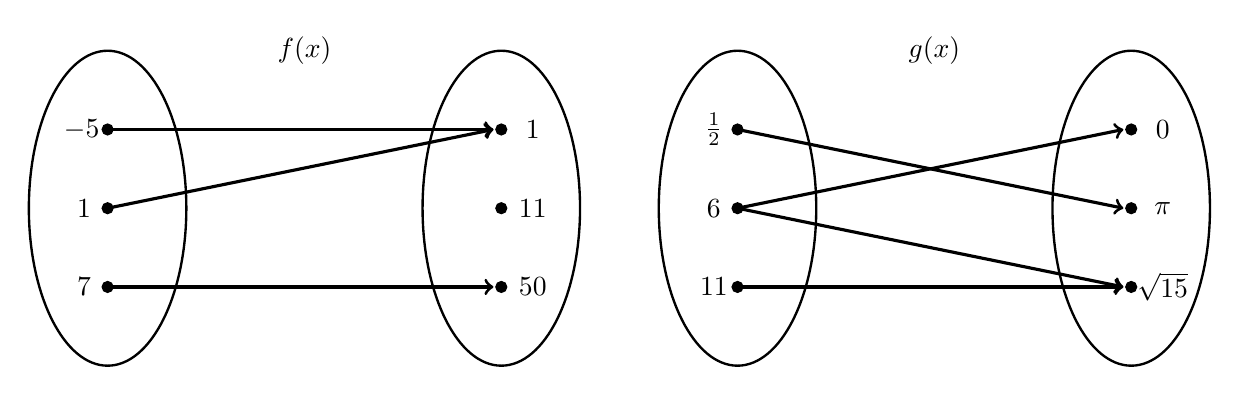
\begin{tikzpicture}
	\node at (2.5,2) {$f(x)$};
	% Ellipses
	\draw[line width=0.03cm] (0,0) circle (1 and 2);
	\draw[line width=0.03cm] (5,0) circle (1 and 2);
	
	% Nodes
	\draw[fill=black] (0,1) circle (0.07);
	\draw[fill=black] (0,0) circle (0.07);
	\draw[fill=black] (0,-1) circle (0.07);
	
	\draw[fill=black] (5,1) circle (0.07);
	\draw[fill=black] (5,0) circle (0.07);
	\draw[fill=black] (5,-1) circle (0.07);
	
	% Arrow
	\draw[line width=0.04cm,->] (0,1) -- (4.9,1);
	\draw[line width=0.04cm,->] (0,0) -- (4.9,1);
	\draw[line width=0.04cm,->] (0,-1) -- (4.9,-1);
	
	% Labels
	\node at (-0.3,1) {$\!-5$};
	\node at (-0.3,0) {$1$};
	\node at (-0.3,-1) {$7$};
	
	\node at (5.4,1) {$1$};
	\node at (5.4,0) {$11$};
	\node at (5.4,-1) {$50$};
	
	\tikzset{shift={(8,0)}}
	%
	\node at (2.5,2) {$g(x)$};
	% Ellipses
	\draw[line width=0.03cm] (0,0) circle (1 and 2);
	\draw[line width=0.03cm] (5,0) circle (1 and 2);
	
	% Nodes
	\draw[fill=black] (0,1) circle (0.07);
	\draw[fill=black] (0,0) circle (0.07);
	\draw[fill=black] (0,-1) circle (0.07);
	
	\draw[fill=black] (5,1) circle (0.07);
	\draw[fill=black] (5,0) circle (0.07);
	\draw[fill=black] (5,-1) circle (0.07);
	
	% Arrow
	\draw[line width=0.04cm,->] (0,1) -- (4.9,0);
	\draw[line width=0.04cm,->] (0,0) -- (4.9,1);
	\draw[line width=0.04cm,->] (0,0) -- (4.9,-1);
	\draw[line width=0.04cm,->] (0,-1) -- (4.9,-1);
	
	% Labels
	\node at (-0.3,1) {$\frac{1}{2}$};
	\node at (-0.3,0) {$6$};
	\node at (-0.3,-1) {$11$};
	
	\node at (5.4,1) {$0$};
	\node at (5.4,0) {$\pi$};
	\node at (5.4,-1) {$\sqrt{15}$};
	\end{tikzpicture}
	\] \pspace


% Problem
\prob Suppose $f(x)$ and $g(x)$ are the functions given below. 
        \begin{table}[H]
        \centering
        \begin{tabular}{| c || r | r | r | r | r | r | r |} \hline
	$x$ & $-3$ & $-2$ & $-1$ & $\phantom{-}0$ & $\phantom{-}1$ & $\phantom{-}2$ & $\phantom{-}3$ \\ \hline \hline
	$f(x)$ & $6$ & $0$ & $-4$ & $5$ & $4$ & $-3$ & $2$ \\ \hline
	$g(x)$ & $0$ & $3$ & $1$ & $1$ & $2$ & $9$ & $6$ \\ \hline
	$h(x)$ & $-1$ & $5$ & $-8$ & $-3$ & $8$ & $2$ & $0$ \\ \hline
        \end{tabular}
        \end{table}

Compute the following: \pspace
        \begin{enumerate}[(a)]
        \item $(g + h)(1)=$ 
        \item $(g - f)(0)=$ 
        \item $(-2h)(3)=$ 
        \item $\left(\dfrac{h}{g}\right)(2)=$ 
        \item $f(1)\, h(-1)=$ 
        \item $f(-1 - h(0))=$ 
        \item $(f \circ g)(-2)=$ 
	\item $(g \circ h)(-3)=$ 
        \item $(h \circ g)(-3)=$ 
	\item $(h \circ f \circ g)(1)=$ 
        \end{enumerate} \pspace


% Problem
\prob Suppose $f(x)$ and $g(x)$ are the functions given below. 
	\[
	\begin{aligned}
	f(x)&= 5x - 6 \\[0.3cm]
	g(x)&= 3x + 1
	\end{aligned}
	\]

Compute the following: \pspace
        \begin{enumerate}[(a)]
        \item $g(2)=$ 
        \item $f(-1)=$ 
        \item $2f(1) - g(2)=$ 
        \item $f(x) - g(x)=$ 
        \item $f(x) \, g(x)=$ 
        \item $\left( \dfrac{f}{g} \right)(x)=$ 
        \item $(f \circ g)(0)=$ 
        \item $(g \circ f)(1)=$ 
        \item $(f \circ g)(x)=$ 
        \item $(g \circ f)(x)=$ 
        \end{enumerate} \pspace


% Problem
\prob Determine if the relation below is a function or not. If it is a function, explain why. If it is not a function, explain why. 
	\[
	\fbox{
	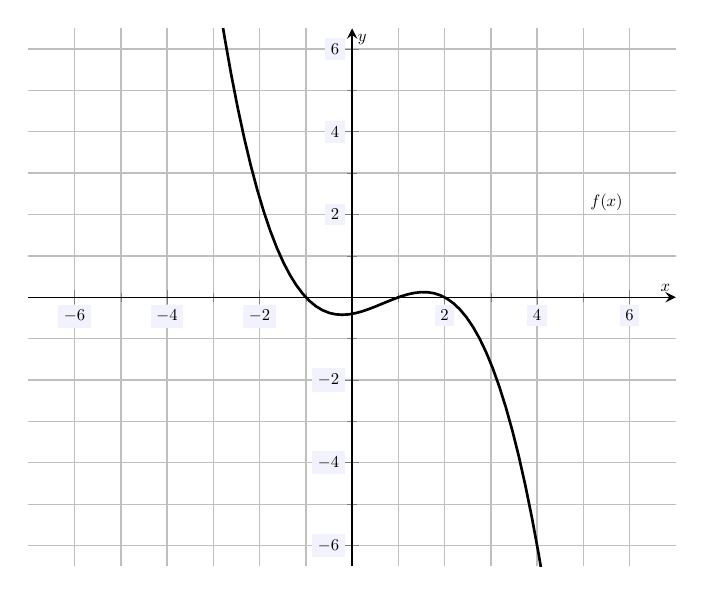
\begin{tikzpicture}[scale=1.2,every node/.style={scale=0.5}]
	\begin{axis}[
	grid=both,
	axis lines=middle,
	ticklabel style={fill=blue!5!white},
	xmin= -7, xmax=7,
	ymin= -6.5, ymax=6.5,
	xtick={-6,-4,-2,0,2,4,6},
	ytick={-6,-4,-2,0,2,4,6},
	minor tick = {-5,-3,...,5},
	xlabel=\(x\),ylabel=\(y\),
	]
	\node at (5.5,2.3) {$f(x)$};
	\addplot[thick, domain= -7:7, samples=100] ({x},{-1/5*(x + 1)*(x - 2)*(x -1)});
	\end{axis}
	\end{tikzpicture}
	}
	\] \pspace


% Problem
\prob  Determine whether the point $(3, -4)$ is on the graph of $f(x)= \dfrac{x + 1}{x - 4}$. Determine also whether the point $(9, -2)$ is on the graph of $f(x)$. For each, explain why or why not. \pspace


% Problem
\prob Explain why the function sketched below has an inverse and then sketch its inverse. 
	\[
	\fbox{
	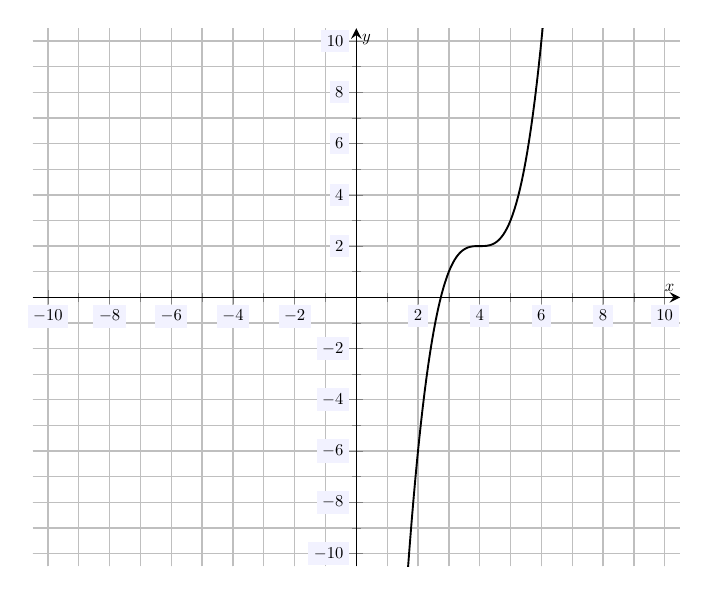
\begin{tikzpicture}[scale=1.2,every node/.style={scale=0.5}]
	\begin{axis}[
	grid=both,
	axis lines=middle,
	ticklabel style={fill=blue!5!white},
	xmin= -10.5, xmax=10.5,
	ymin= -10.5, ymax=10.5,
	xtick={-10,-8,-6,-4,-2,0,2,4,6,8,10},
	ytick={-10,-8,-6,-4,-2,0,2,4,6,8,10},
	minor tick = {-10,-9,...,10},
	xlabel=\(x\),ylabel=\(y\),
	]
	\addplot[line width= 0.02cm,domain= 1:7, samples=100] ({x},{(x - 4)^3 + 2}); 
	\end{axis}
	\end{tikzpicture}
	}
	\] \pspace


% Problem
\prob How many $y$-intercepts can a function have? Explain. Is this the same for $x$-intercepts? Explain. \pspace


% Problem
\prob Using the concept of range and the fact that every non-horizontal line $\ell(x)$ intersects any horizontal line, explain why the equation $\ell(x)= c$ has a solution for every real number $c$. \pspace


% Problem
\prob Define what makes a function linear. What `form' does every linear function of one-variable have? \pspace


% Problem
\prob Being as accurate as possible, sketch the graph of the line $-3x + 5y= 10$.
	\[
	\fbox{
	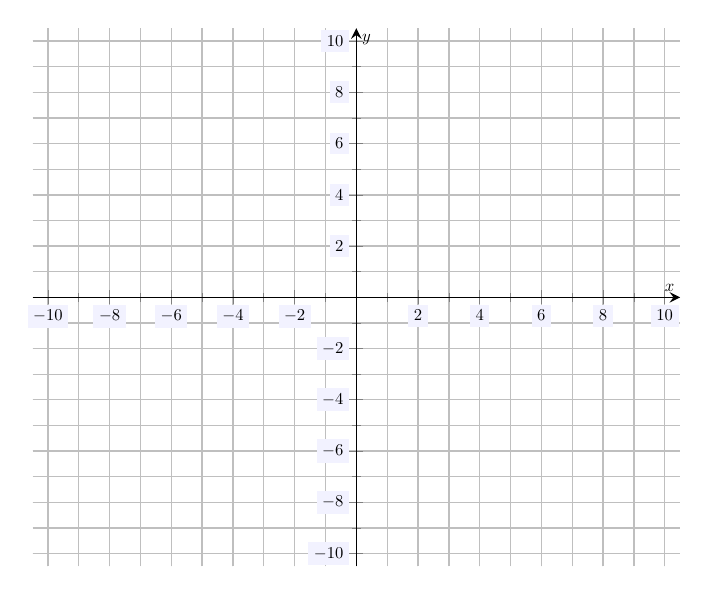
\begin{tikzpicture}[scale=1.2,every node/.style={scale=0.5}]
	\begin{axis}[
	grid=both,
	axis lines=middle,
	ticklabel style={fill=blue!5!white},
	xmin= -10.5, xmax=10.5,
	ymin= -10.5, ymax=10.5,
	xtick={-10,-8,-6,-4,-2,0,2,4,6,8,10},
	ytick={-10,-8,-6,-4,-2,0,2,4,6,8,10},
	minor tick = {-10,-9,...,10},
	xlabel=\(x\),ylabel=\(y\),
	]
	\end{axis}
	\end{tikzpicture}
	}
	\] \pspace





\newpage





% Problem
\prob  Determine if the following function is linear. Explain why or why not.
	\begin{table}[H]
	\centering
	\begin{tabular}{c|c}
	$x$ & $f(x)$ \\ \hline
	$0.5$ & $26.45$ \\
	$1.8$ & $21.64$ \\
	$3.9$ & $13.87$ \\
	$4.2$ & $13.44$ \\
	$5.5$ & $7.95$ \\
	$8.1$ & $-1.67$
	\end{tabular}
	\end{table} \pspace


% Problem
\prob Consider the linear equation $15x + 3y= 39$. 
        \begin{enumerate}[(a)]
        \item Solve the linear equation for $y$. 
        \item Determine the slope and $y$-intercept for the corresponding line.
        \item Interpret the slope in at least two different ways. 
        \end{enumerate} \pspace


% Problem
\prob Consider the line given by $y= \frac{11}{4}\,x - 6$.
        \begin{enumerate}[(a)]
        \item Put the line in standard form.
        \item Is the point $(-12, -27)$ on the line? Explain.
        \item Is the point $(8, 16)$ on the line? Explain. 
        \end{enumerate} \pspace


% Problem
\prob A linear function has a table whose values are given below. Find the equation of the linear function. Be sure to specify the slope and $y$-intercept.
	\begin{table}[H]
	\centering
	\begin{tabular}{c|c}
	$x$ & $f(x)$ \\ \hline
	$3$ & $5.7$ \\ 
	$4$ & $2.4$ \\
	$7$ & $-7.5$ \\
	$11$ & $-20.7$
	\end{tabular}
	\end{table} \pspace


% Problem
\prob You are driving back to college after summer break. It is 12~pm and you are traveling on the highway at a constant speed of 65~mph. Currently, you are 211~mi from college. Let $D(t)$ denote your distance, in miles, that you are from the college $t$ hours from now. 
	\begin{enumerate}[(a)]
	\item Explain why $D(t)$ is linear.
	\item Find $D(t)$. 
	\item What do the slope and $y$-intercept of $W(t)$ represent in context?
	\item Determine when you will arrive at the college. 
	\end{enumerate} \pspace


% Problem
\prob Showing all your work, find the equation of the line with slope $-\frac{1}{3}$ that passes through the point $(9, 4)$. \pspace


% Problem
\prob Showing all your work, find the equation of the line that has $x$-intercept $(-2, 0)$ and $y$-intercept $(0, -5)$. \pspace


% Problem
\prob Determine whether the following lines are parallel, perpendicular, or neither. Be sure to justify your answer. \pvspace{0.1cm}
	\[
	\begin{aligned}
	\ell_1 &\colon y= \dfrac{2}{3}\,x + 5 \\[0.3cm]
	\ell_2 &\colon 3x - 2y= 8
	\end{aligned}
	\] \pspace


% Problem
\prob Determine whether the following lines are parallel, perpendicular, or neither. Be sure to justify your answer. \pvspace{0.1cm}
	\[
	\begin{aligned}
	\ell_1 &\colon -5x + 6y= 6 \\[0.3cm]
	\ell_2 &\colon 5x + 6y= -12
	\end{aligned}
	\] \pspace


% Problem
\prob Find the equation of the line with $x$-intercept $(6, 0)$ and passing through the point $(-1, 10)$. \pspace


% Problem
\prob Find the equation of the line perpendicular to the line $2x - 3y= 5$ that passes through the origin. \pspace


% Problem
\prob Find the equation of the line that contains $(1, -1)$ and is parallel to the line $3x + y= 11$. \pspace


% Problem
\prob Showing all your work, solve the following equation and verify that your solution is correct:
	\[
	5x - 7= 7 - 2x
	\] \pspace


% Problem
\prob Showing all your work, solve the following equation and verify that your solution is correct:
	\[
	2(1 - x)= 6x + 11
	\] \pspace


% Problem
\prob Showing all your work, solve the following equation and verify that your solution is correct:
	\[
	\dfrac{x - 1}{x + 3}= 5
	\] \pspace


% Problem 
\prob Suppose you sell automobiles. You earn a weekly baseline salary of \$820 per week and make 3\% commission on your sales. Let $I(s)$ denote your weekly income if you make $s$~dollars in sales. 
	\begin{enumerate}[(a)]
	\item Explain why $I(s)$ is linear. 
	\item Find $I(s)$.
	\item Find and interpret the slope and $y$-intercept of $I(s)$ in context, if possible. 
	\item How much in sales do you have to make in a given week to have made \$1,500?
	\end{enumerate} \pspace


\end{document}